\documentclass[]{article}
\usepackage{lmodern}
\usepackage{amssymb,amsmath}
\usepackage{ifxetex,ifluatex}
\usepackage{fixltx2e} % provides \textsubscript
\ifnum 0\ifxetex 1\fi\ifluatex 1\fi=0 % if pdftex
  \usepackage[T1]{fontenc}
  \usepackage[utf8]{inputenc}
\else % if luatex or xelatex
  \ifxetex
    \usepackage{mathspec}
  \else
    \usepackage{fontspec}
  \fi
  \defaultfontfeatures{Ligatures=TeX,Scale=MatchLowercase}
\fi
% use upquote if available, for straight quotes in verbatim environments
\IfFileExists{upquote.sty}{\usepackage{upquote}}{}
% use microtype if available
\IfFileExists{microtype.sty}{%
\usepackage{microtype}
\UseMicrotypeSet[protrusion]{basicmath} % disable protrusion for tt fonts
}{}
\usepackage[margin=1in]{geometry}
\usepackage{hyperref}
\hypersetup{unicode=true,
            pdftitle={Lecture Notes for Statistics for Biology FS2020},
            pdfauthor={Stephan Peischl},
            pdfborder={0 0 0},
            breaklinks=true}
\urlstyle{same}  % don't use monospace font for urls
\usepackage{color}
\usepackage{fancyvrb}
\newcommand{\VerbBar}{|}
\newcommand{\VERB}{\Verb[commandchars=\\\{\}]}
\DefineVerbatimEnvironment{Highlighting}{Verbatim}{commandchars=\\\{\}}
% Add ',fontsize=\small' for more characters per line
\usepackage{framed}
\definecolor{shadecolor}{RGB}{248,248,248}
\newenvironment{Shaded}{\begin{snugshade}}{\end{snugshade}}
\newcommand{\AlertTok}[1]{\textcolor[rgb]{0.94,0.16,0.16}{#1}}
\newcommand{\AnnotationTok}[1]{\textcolor[rgb]{0.56,0.35,0.01}{\textbf{\textit{#1}}}}
\newcommand{\AttributeTok}[1]{\textcolor[rgb]{0.77,0.63,0.00}{#1}}
\newcommand{\BaseNTok}[1]{\textcolor[rgb]{0.00,0.00,0.81}{#1}}
\newcommand{\BuiltInTok}[1]{#1}
\newcommand{\CharTok}[1]{\textcolor[rgb]{0.31,0.60,0.02}{#1}}
\newcommand{\CommentTok}[1]{\textcolor[rgb]{0.56,0.35,0.01}{\textit{#1}}}
\newcommand{\CommentVarTok}[1]{\textcolor[rgb]{0.56,0.35,0.01}{\textbf{\textit{#1}}}}
\newcommand{\ConstantTok}[1]{\textcolor[rgb]{0.00,0.00,0.00}{#1}}
\newcommand{\ControlFlowTok}[1]{\textcolor[rgb]{0.13,0.29,0.53}{\textbf{#1}}}
\newcommand{\DataTypeTok}[1]{\textcolor[rgb]{0.13,0.29,0.53}{#1}}
\newcommand{\DecValTok}[1]{\textcolor[rgb]{0.00,0.00,0.81}{#1}}
\newcommand{\DocumentationTok}[1]{\textcolor[rgb]{0.56,0.35,0.01}{\textbf{\textit{#1}}}}
\newcommand{\ErrorTok}[1]{\textcolor[rgb]{0.64,0.00,0.00}{\textbf{#1}}}
\newcommand{\ExtensionTok}[1]{#1}
\newcommand{\FloatTok}[1]{\textcolor[rgb]{0.00,0.00,0.81}{#1}}
\newcommand{\FunctionTok}[1]{\textcolor[rgb]{0.00,0.00,0.00}{#1}}
\newcommand{\ImportTok}[1]{#1}
\newcommand{\InformationTok}[1]{\textcolor[rgb]{0.56,0.35,0.01}{\textbf{\textit{#1}}}}
\newcommand{\KeywordTok}[1]{\textcolor[rgb]{0.13,0.29,0.53}{\textbf{#1}}}
\newcommand{\NormalTok}[1]{#1}
\newcommand{\OperatorTok}[1]{\textcolor[rgb]{0.81,0.36,0.00}{\textbf{#1}}}
\newcommand{\OtherTok}[1]{\textcolor[rgb]{0.56,0.35,0.01}{#1}}
\newcommand{\PreprocessorTok}[1]{\textcolor[rgb]{0.56,0.35,0.01}{\textit{#1}}}
\newcommand{\RegionMarkerTok}[1]{#1}
\newcommand{\SpecialCharTok}[1]{\textcolor[rgb]{0.00,0.00,0.00}{#1}}
\newcommand{\SpecialStringTok}[1]{\textcolor[rgb]{0.31,0.60,0.02}{#1}}
\newcommand{\StringTok}[1]{\textcolor[rgb]{0.31,0.60,0.02}{#1}}
\newcommand{\VariableTok}[1]{\textcolor[rgb]{0.00,0.00,0.00}{#1}}
\newcommand{\VerbatimStringTok}[1]{\textcolor[rgb]{0.31,0.60,0.02}{#1}}
\newcommand{\WarningTok}[1]{\textcolor[rgb]{0.56,0.35,0.01}{\textbf{\textit{#1}}}}
\usepackage{graphicx,grffile}
\makeatletter
\def\maxwidth{\ifdim\Gin@nat@width>\linewidth\linewidth\else\Gin@nat@width\fi}
\def\maxheight{\ifdim\Gin@nat@height>\textheight\textheight\else\Gin@nat@height\fi}
\makeatother
% Scale images if necessary, so that they will not overflow the page
% margins by default, and it is still possible to overwrite the defaults
% using explicit options in \includegraphics[width, height, ...]{}
\setkeys{Gin}{width=\maxwidth,height=\maxheight,keepaspectratio}
\IfFileExists{parskip.sty}{%
\usepackage{parskip}
}{% else
\setlength{\parindent}{0pt}
\setlength{\parskip}{6pt plus 2pt minus 1pt}
}
\setlength{\emergencystretch}{3em}  % prevent overfull lines
\providecommand{\tightlist}{%
  \setlength{\itemsep}{0pt}\setlength{\parskip}{0pt}}
\setcounter{secnumdepth}{0}
% Redefines (sub)paragraphs to behave more like sections
\ifx\paragraph\undefined\else
\let\oldparagraph\paragraph
\renewcommand{\paragraph}[1]{\oldparagraph{#1}\mbox{}}
\fi
\ifx\subparagraph\undefined\else
\let\oldsubparagraph\subparagraph
\renewcommand{\subparagraph}[1]{\oldsubparagraph{#1}\mbox{}}
\fi

%%% Use protect on footnotes to avoid problems with footnotes in titles
\let\rmarkdownfootnote\footnote%
\def\footnote{\protect\rmarkdownfootnote}

%%% Change title format to be more compact
\usepackage{titling}

% Create subtitle command for use in maketitle
\newcommand{\subtitle}[1]{
  \posttitle{
    \begin{center}\large#1\end{center}
    }
}

\setlength{\droptitle}{-2em}

  \title{Lecture Notes for Statistics for Biology FS2020}
    \pretitle{\vspace{\droptitle}\centering\huge}
  \posttitle{\par}
    \author{Stephan Peischl}
    \preauthor{\centering\large\emph}
  \postauthor{\par}
      \predate{\centering\large\emph}
  \postdate{\par}
    \date{1/10/2020}


\begin{document}
\maketitle

{
\setcounter{tocdepth}{2}
\tableofcontents
}
\hypertarget{introduction}{%
\section{Introduction}\label{introduction}}

These notes should help you get started with the statistics software R,
guide you through the practical part of the course and provide
additional information on selected topics. Before you continue reading,
make sure you have R and R Studio installed on your computer. Try to use
R as an calcualtor as shown in the lecture slides and try to get yourelf
acustomed to the different windows in the R Studio envrionment. No prior
knwoledge about R is necessary and once everything is up and running yu
can dive right in.

We start by loading some relevant packages for this course. An R package
is a collection of functions, data, and documentation that extends the
capabilities of base R.

\begin{Shaded}
\begin{Highlighting}[]
\CommentTok{# make sure you have th packages installed using }
\CommentTok{# install.packages(packagename)}

\KeywordTok{library}\NormalTok{(tidyverse)}
\KeywordTok{library}\NormalTok{(Rmisc)}
\KeywordTok{library}\NormalTok{(tibble)}
\KeywordTok{library}\NormalTok{(dplyr)}


\CommentTok{# here i define a color palette to use as standard when plotting with ggplot}
\CommentTok{# this is purely for aesthetic reasons }

\NormalTok{cbp2 <-}\StringTok{ }\KeywordTok{c}\NormalTok{(}\StringTok{"#000000"}\NormalTok{, }\StringTok{"#E69F00"}\NormalTok{, }\StringTok{"#56B4E9"}\NormalTok{, }\StringTok{"#009E73"}\NormalTok{,}
          \StringTok{"#F0E442"}\NormalTok{, }\StringTok{"#0072B2"}\NormalTok{, }\StringTok{"#D55E00"}\NormalTok{, }\StringTok{"#CC79A7"}\NormalTok{)}

\NormalTok{scale_colour_discrete <-}\StringTok{ }\ControlFlowTok{function}\NormalTok{(...) \{}
  \KeywordTok{scale_colour_manual}\NormalTok{(..., }\DataTypeTok{values =}\NormalTok{ cbp2)}
\NormalTok{\}}
\end{Highlighting}
\end{Shaded}

\hypertarget{visualizations-with-ggplot2-and-base-r}{%
\section{Visualizations with ggplot2 and base
R}\label{visualizations-with-ggplot2-and-base-r}}

\hypertarget{ggplot-2}{%
\subsection{GGplot 2}\label{ggplot-2}}

We start with some examples of how to visulaize data quickly and easily.
This should show you how to produce high quality visulaizations using R
and motivate you to learn more about programming and data analysis with
R.

R has several systems for making graphs, and I have chosen to start with
ggplot2 beacuse it is elegant, versatile and is easy to leanr if you
have no prior knowledge about programming. For those of you who are
already familiar wiht programming langauges, doing graphics in ``base
R'' may seem more intuitive initially but I hope I can convince you that
the grammar of plotting used by ggplot has lots of advantages and is
very readable once you get the hang of it.

If you like to learn more about the theoretical underpinnings of ggplot2
before you start, I???d recommend reading ``The Layered Grammar of
Graphics'', \url{http://vita.had.co.nz/papers/layered-grammar.pdf}.

\hypertarget{the-mpg-dataset}{%
\subsubsection{The MPG dataset}\label{the-mpg-dataset}}

Let us use our first graph to answer a question: Do cars with big
engines use more fuel than cars with small engines? What does the
relationship between engine size and fuel efficiency look like? Is it
positive? Negative? Linear? Nonlinear?

We can find an answer with the mpg data set found in ggplot2 (aka
ggplot2::mpg). A data frame is the R data format to store data in a
spreadsheet: a rectangular collection of variables (in the columns) and
observations (in the rows). The data frame mpg contains observations
collected by the US Environmental Protection Agency on 38 models of car.

\begin{Shaded}
\begin{Highlighting}[]
\CommentTok{# the command head() shos us the first few rows of the data set to }
\CommentTok{# get an overview of what is stored in our dataset}

\KeywordTok{head}\NormalTok{(mpg)}
\end{Highlighting}
\end{Shaded}

\begin{verbatim}
## # A tibble: 6 x 11
##   manufacturer model displ  year   cyl trans drv     cty   hwy fl    class
##   <chr>        <chr> <dbl> <int> <int> <chr> <chr> <int> <int> <chr> <chr>
## 1 audi         a4      1.8  1999     4 auto~ f        18    29 p     comp~
## 2 audi         a4      1.8  1999     4 manu~ f        21    29 p     comp~
## 3 audi         a4      2    2008     4 manu~ f        20    31 p     comp~
## 4 audi         a4      2    2008     4 auto~ f        21    30 p     comp~
## 5 audi         a4      2.8  1999     6 auto~ f        16    26 p     comp~
## 6 audi         a4      2.8  1999     6 manu~ f        18    26 p     comp~
\end{verbatim}

Among the variables in mpg are:

\textbf{displ}, a car???s engine size, in litres.

\textbf{hwy}, a car???s fuel efficiency on the highway, in miles per
gallon (mpg). A car with a low fuel efficiency consumes more fuel than a
car with a high fuel efficiency when they travel the same distance.

To learn more about mpg, open its help page by running ?mpg. in the next
seciton we learn how to visualize such data.

\hypertarget{the-grammar-of-ggplot2}{%
\subsubsection{The grammar of ggplot2}\label{the-grammar-of-ggplot2}}

In general you begin a plot with the function \emph{ggplot()}. ggplot()
creates a coordinate system that you can add layers to. The first
argument of ggplot() is the dataset to use in the graph. For instance,
typing ggplot(data = mpg) into the console creates an empty graph (which
is boring so it is not shown here). You can now add layers to your plot.
For example, the function geom\_point() adds a layer of points to your
plot, thus creating a scatterplot.

\begin{Shaded}
\begin{Highlighting}[]
\KeywordTok{ggplot}\NormalTok{(}\DataTypeTok{data =}\NormalTok{ mpg) }\OperatorTok{+}\StringTok{ }
\StringTok{  }\KeywordTok{geom_point}\NormalTok{(}\DataTypeTok{mapping =} \KeywordTok{aes}\NormalTok{(}\DataTypeTok{x =}\NormalTok{ displ, }\DataTypeTok{y =}\NormalTok{ hwy)) }
\end{Highlighting}
\end{Shaded}

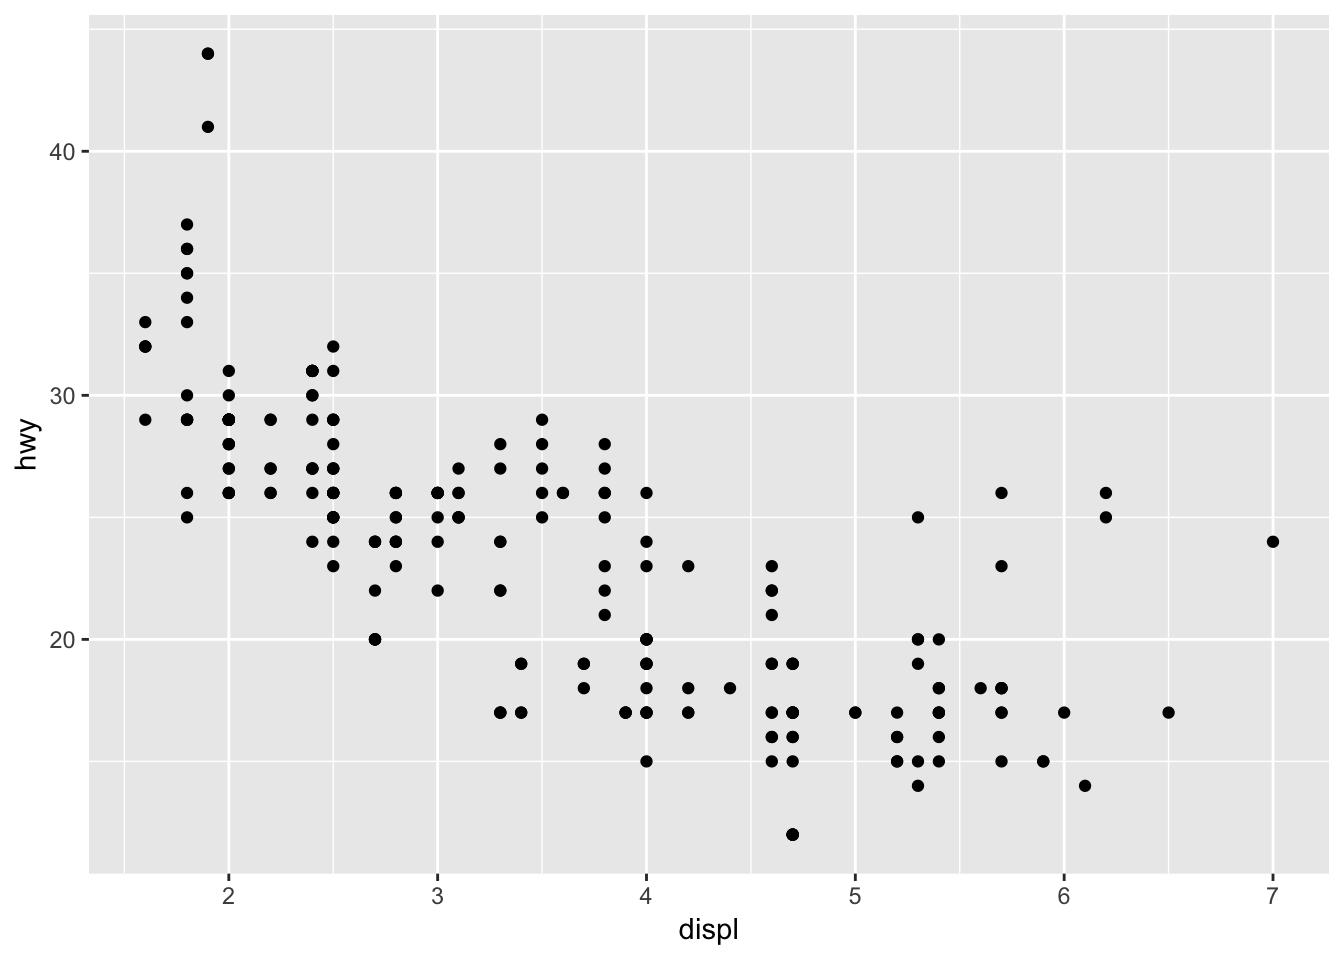
\includegraphics{index_files/figure-latex/mileage-1.pdf}

There are many other such \emph{geometric functions} withing the ggplot2
universe and you can combine them in a single plot. You will learn a
whole bunch of them throughout this course, but be aware that we will
only scratch the surface of what is available. After this course, you
should be ready to equip your self with new tools for data analysis
whenever you need them.

Each geom function in ggplot2 takes a mapping argument. This defines how
variables in your dataset are mapped to visual properties. The mapping
argument is always paired with aes(), and the x and y arguments of aes()
specify which variables to map to the x and y axes. ggplot2 looks for
the mapped variables in the data argument, in this case, mpg.

Next, we use a different theme beacuse this gray background in the
standard design is ugly.

\begin{Shaded}
\begin{Highlighting}[]
\KeywordTok{ggplot}\NormalTok{(}\DataTypeTok{data =}\NormalTok{ mpg) }\OperatorTok{+}\StringTok{ }
\StringTok{  }\KeywordTok{geom_point}\NormalTok{(}\DataTypeTok{mapping =} \KeywordTok{aes}\NormalTok{(}\DataTypeTok{x =}\NormalTok{ displ, }\DataTypeTok{y =}\NormalTok{ hwy)) }\OperatorTok{+}
\StringTok{  }\KeywordTok{theme_classic}\NormalTok{()}
\end{Highlighting}
\end{Shaded}

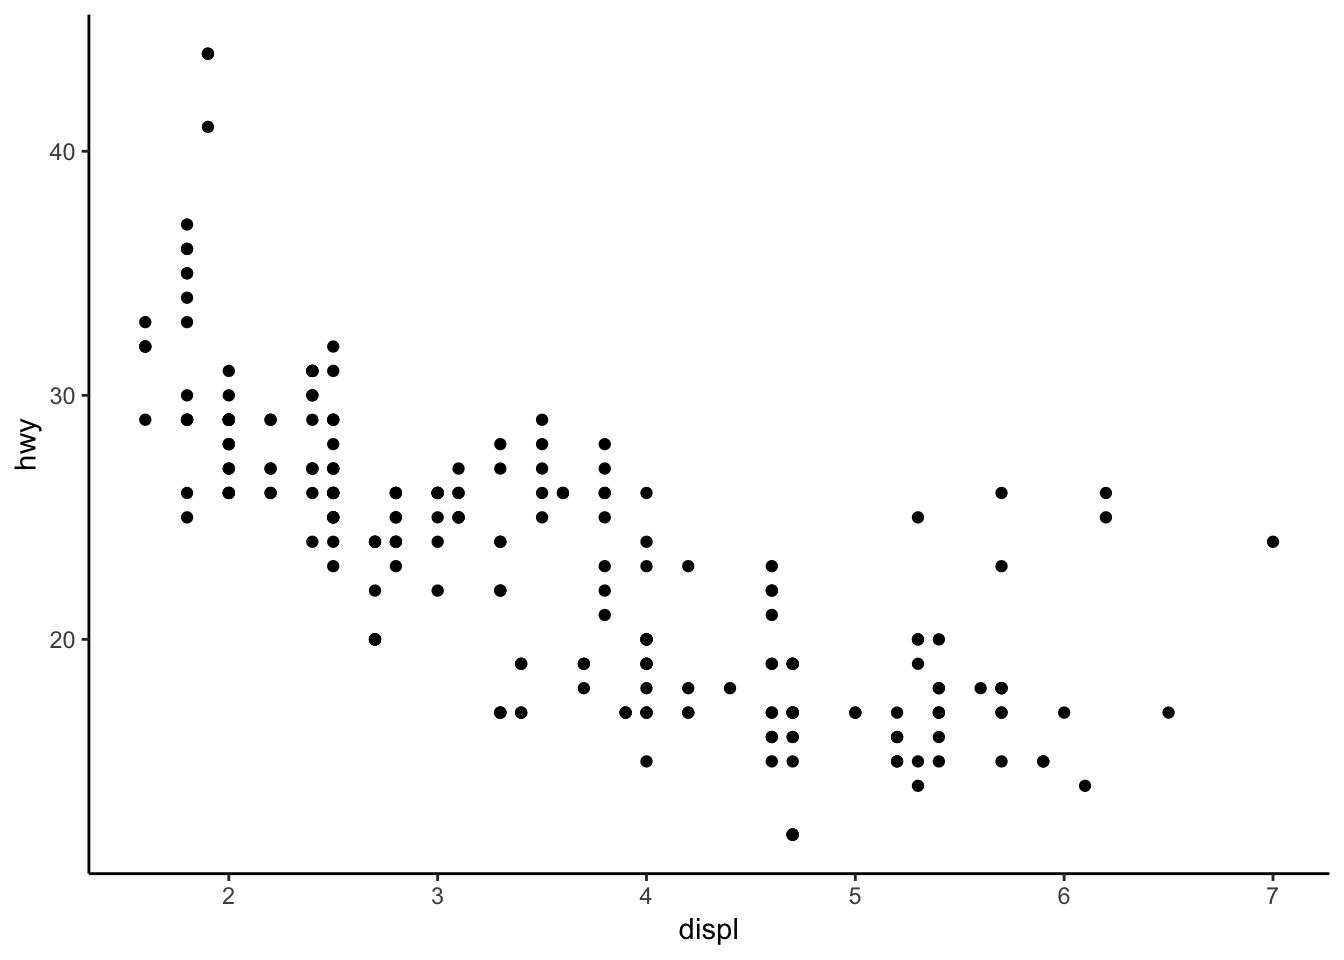
\includegraphics{index_files/figure-latex/mileage2-1.pdf}

The general grammar of ggplot is

ggplot(data = \textless{}DATA\textgreater{}) +

\textless{}GEOM\_FUNCTION\textgreater{}(mapping =
aes(\textless{}MAPPINGS\textgreater{}))

We will explain each part step by step in examples. The DATA argument
should be quite clear: here you specify the dataframe (we will learn
more about that alter) that you want to work with.

The second part, GEOM\_FUNCTION, specifies what kind of plot you want.
As mentioned above \emph{geom\_point} gives you a classic scatter plot.
Many other such funtions exist and we will encounter some of them.

Finally, MAPPING specifies which variables hould be plotted. We ussually
specify this with an aesthetics mapping of the form \emph{mapping =
aes(x = \ldots{}, y =\ldots{})} to deterimne the variables that give us
the x- and y-coordinates. We can however also change the aesthetics of
our plot in various way, for instance by giving data points different
colors that indicate the value of a third variable:

\begin{Shaded}
\begin{Highlighting}[]
\KeywordTok{ggplot}\NormalTok{(}\DataTypeTok{data =}\NormalTok{ mpg) }\OperatorTok{+}\StringTok{ }
\StringTok{  }\KeywordTok{geom_point}\NormalTok{(}\DataTypeTok{mapping =} \KeywordTok{aes}\NormalTok{(}\DataTypeTok{x =}\NormalTok{ displ, }\DataTypeTok{y =}\NormalTok{ hwy,}\DataTypeTok{color =}\NormalTok{ class)) }\OperatorTok{+}
\StringTok{  }\KeywordTok{theme_classic}\NormalTok{()}
\end{Highlighting}
\end{Shaded}

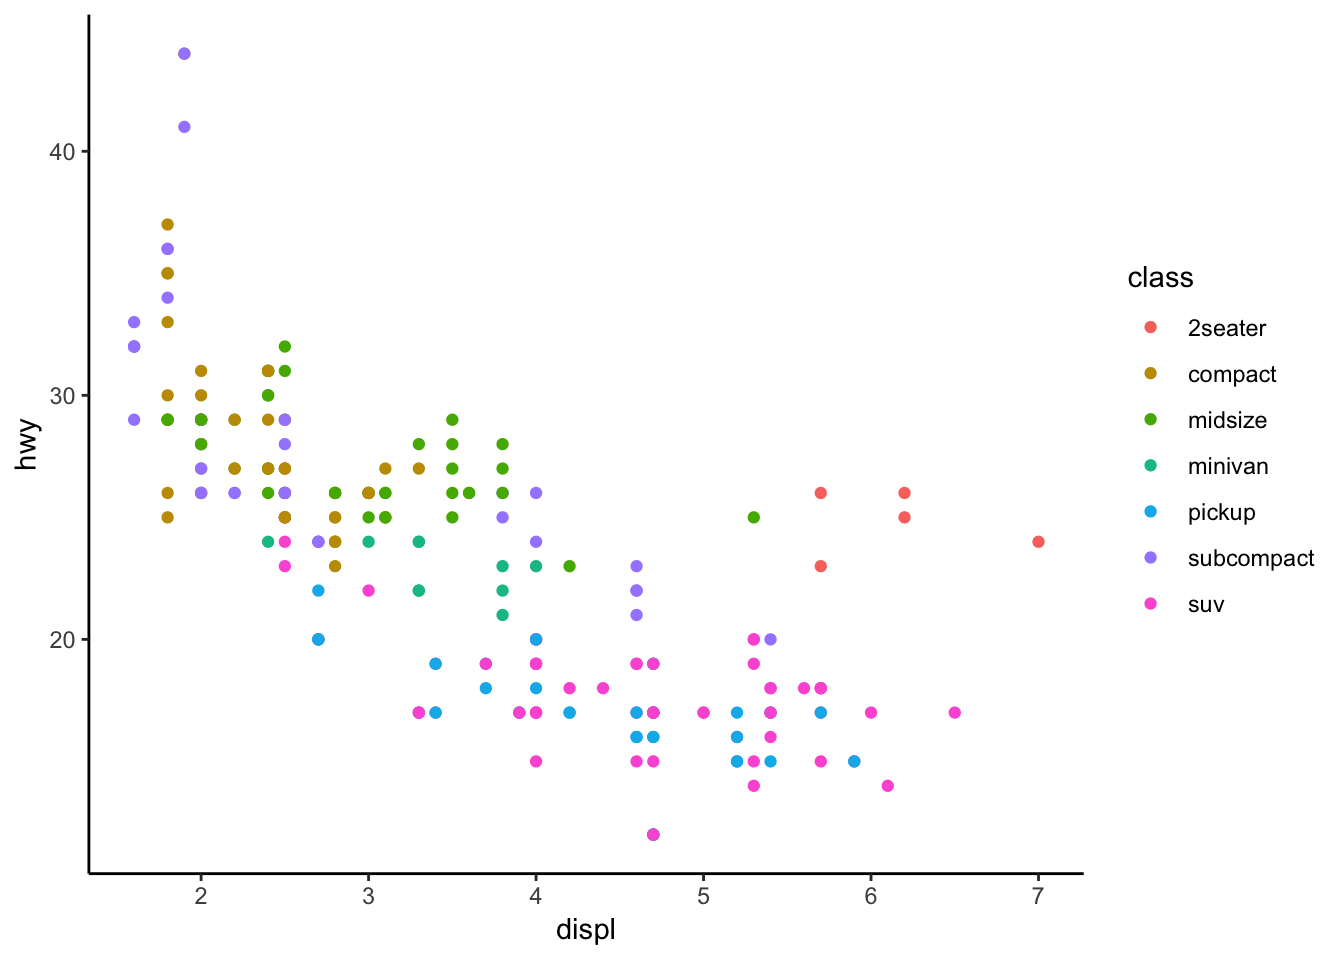
\includegraphics{index_files/figure-latex/mileage_aes-1.pdf}

Another important option is to set a clor manually:

\begin{Shaded}
\begin{Highlighting}[]
\KeywordTok{ggplot}\NormalTok{(}\DataTypeTok{data =}\NormalTok{ mpg) }\OperatorTok{+}\StringTok{ }
\StringTok{  }\KeywordTok{geom_point}\NormalTok{(}\DataTypeTok{mapping =} \KeywordTok{aes}\NormalTok{(}\DataTypeTok{x =}\NormalTok{ displ, }\DataTypeTok{y =}\NormalTok{ hwy), }\DataTypeTok{color =} \StringTok{"blue"}\NormalTok{) }\OperatorTok{+}
\StringTok{  }\KeywordTok{theme_classic}\NormalTok{()}
\end{Highlighting}
\end{Shaded}

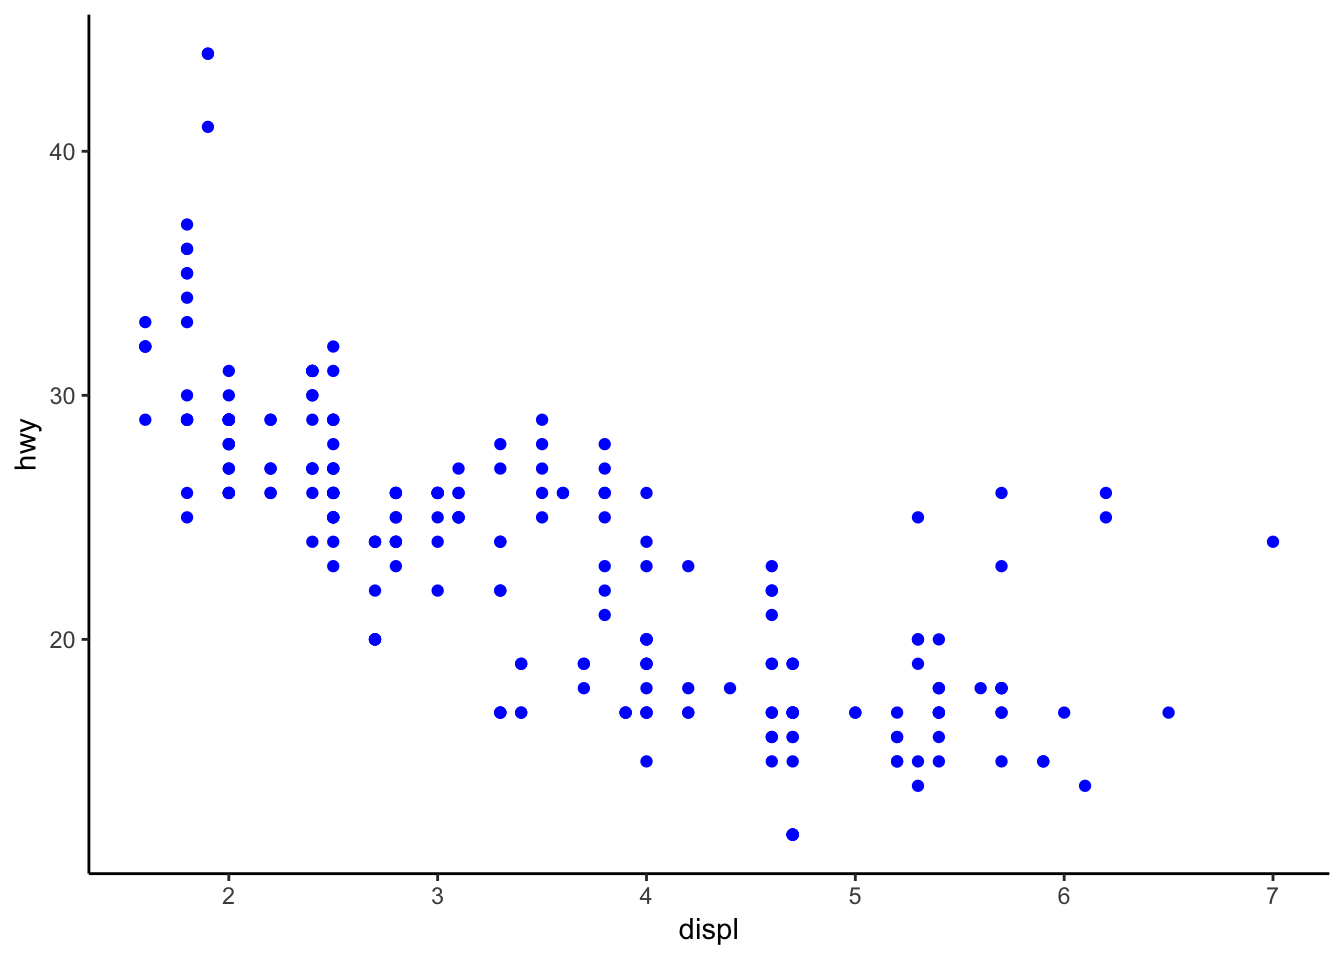
\includegraphics{index_files/figure-latex/mileage_aes_2-1.pdf}

As a final remark, you can also create a plot, store it in a variable
and then explore themes after that:

\begin{Shaded}
\begin{Highlighting}[]
\NormalTok{p =}\StringTok{ }\KeywordTok{ggplot}\NormalTok{(}\DataTypeTok{data =}\NormalTok{ mpg) }\OperatorTok{+}\StringTok{ }
\StringTok{  }\KeywordTok{geom_point}\NormalTok{(}\DataTypeTok{mapping =} \KeywordTok{aes}\NormalTok{(}\DataTypeTok{x =}\NormalTok{ displ, }\DataTypeTok{y =}\NormalTok{ hwy), }\DataTypeTok{color =} \StringTok{"blue"}\NormalTok{) }

\NormalTok{p}\OperatorTok{+}\KeywordTok{theme_classic}\NormalTok{()}
\end{Highlighting}
\end{Shaded}

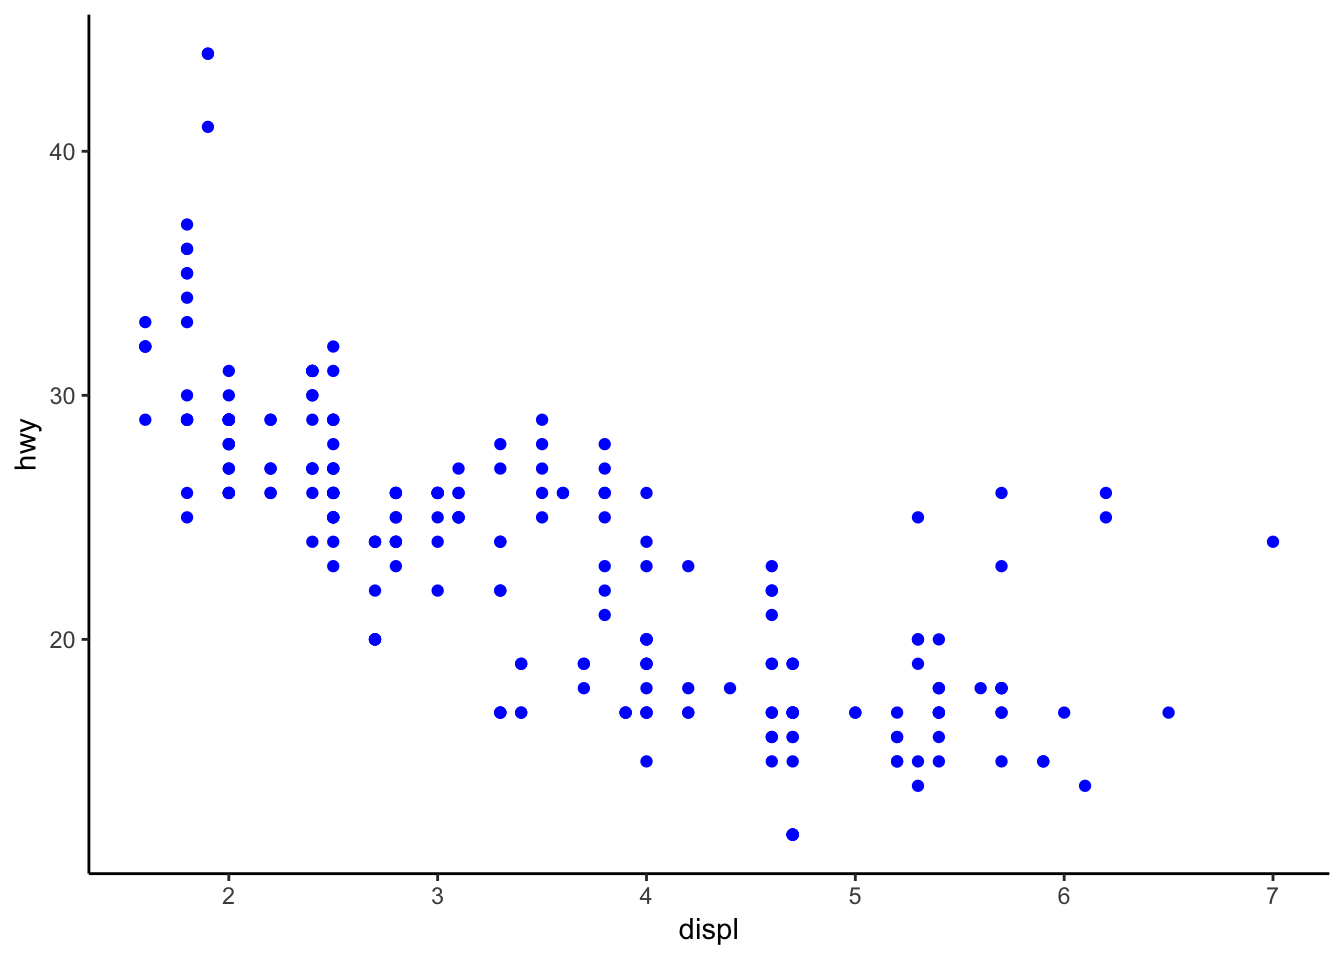
\includegraphics{index_files/figure-latex/mileage_aes_themes-1.pdf}

\begin{Shaded}
\begin{Highlighting}[]
\NormalTok{p}\OperatorTok{+}\KeywordTok{theme_dark}\NormalTok{()}
\end{Highlighting}
\end{Shaded}

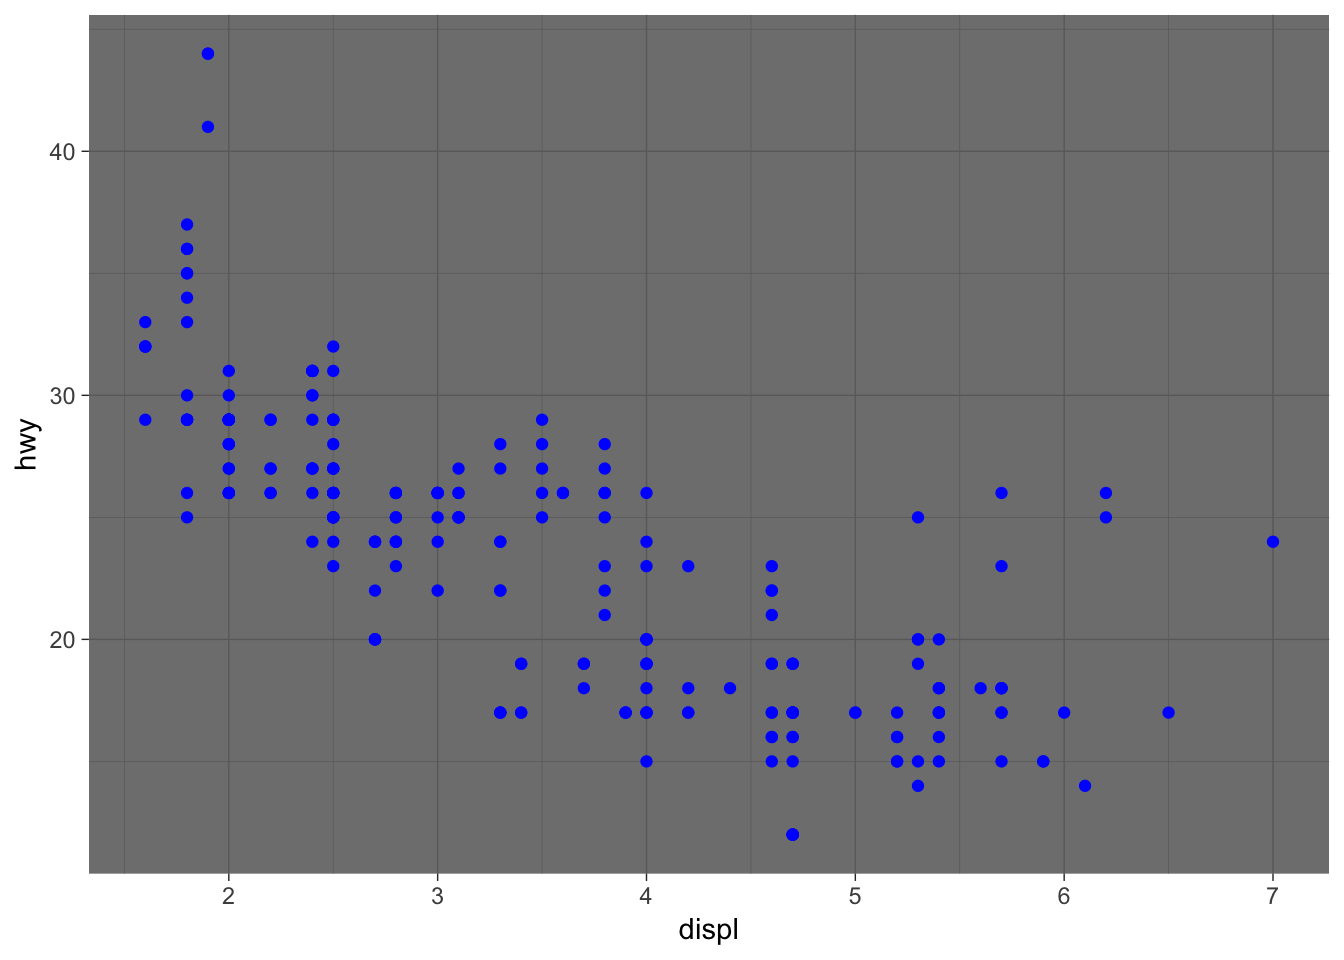
\includegraphics{index_files/figure-latex/mileage_aes_themes-2.pdf}

We now set our prefered them globally, so we do not need to specifiy it
all the time:

\begin{Shaded}
\begin{Highlighting}[]
\KeywordTok{theme_set}\NormalTok{(}\KeywordTok{theme_classic}\NormalTok{())}
\end{Highlighting}
\end{Shaded}

\hypertarget{base-r-graphics}{%
\subsection{Base R graphics}\label{base-r-graphics}}

Base R refers to the standard R functions. While ggplot allows us to
make sophisticated graphs very quickly, I find that in some situations
base R is just as good or even better. Let us recreate the same plot as
before:

\begin{Shaded}
\begin{Highlighting}[]
\KeywordTok{plot}\NormalTok{(mpg}\OperatorTok{$}\NormalTok{displ,mpg}\OperatorTok{$}\NormalTok{hwy) }
\end{Highlighting}
\end{Shaded}

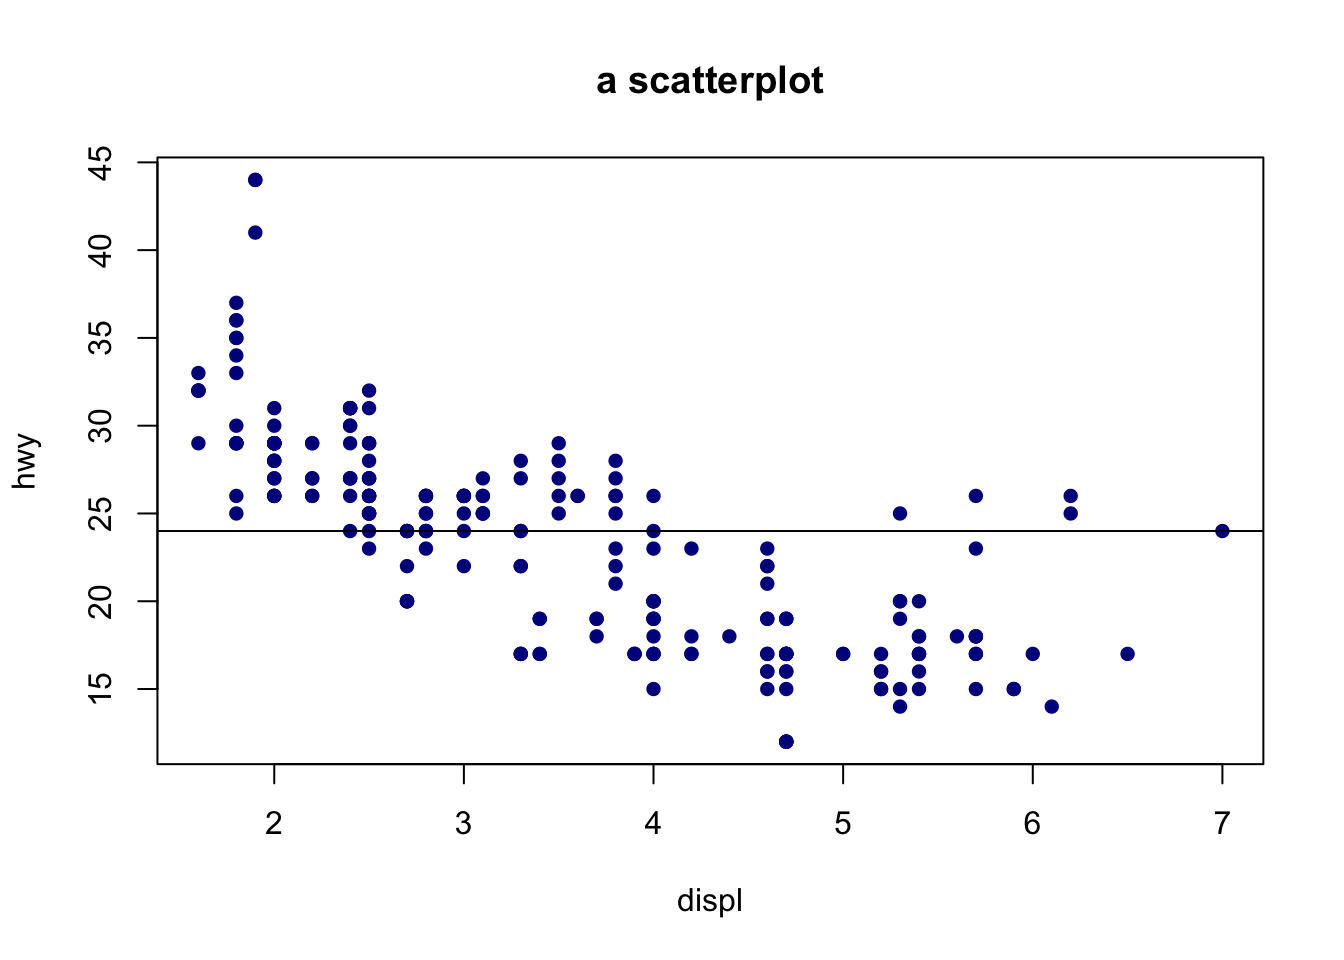
\includegraphics{index_files/figure-latex/unnamed-chunk-2-1.pdf}

Note how we use the \$ symbol to access the variables stored in a data
frame here; it allows you to access a specific column of a data frame.
Try typing the name of a dataframe, followed by the \$ operator in
RStudio; it should automatically suggest you the availbale variable
names in your data frame.

We can alos add stuff to this plot, change colors, and pretty much
everything else we would like to. A quick look at the help function
should give you an overview about the scope of the function plot and
it's parameters. For instance, have a look at the following plot, where
I make a scatterplot and modifiy the appearance of the symbols, add some
labels and a title, and then add a horizontal line at the value of the
median fuel efficiency:

\begin{Shaded}
\begin{Highlighting}[]
\KeywordTok{plot}\NormalTok{(mpg}\OperatorTok{$}\NormalTok{displ,mpg}\OperatorTok{$}\NormalTok{hwy,}\DataTypeTok{pch=}\DecValTok{16}\NormalTok{,}\DataTypeTok{col=}\StringTok{"darkblue"}\NormalTok{,}\DataTypeTok{xlab=}\StringTok{"displ"}\NormalTok{,}\DataTypeTok{ylab=}\StringTok{"hwy"}\NormalTok{, }\DataTypeTok{main =}\StringTok{"a scatterplot"}\NormalTok{)}
\KeywordTok{abline}\NormalTok{(}\DataTypeTok{h =} \KeywordTok{median}\NormalTok{(mpg}\OperatorTok{$}\NormalTok{hwy))}
\end{Highlighting}
\end{Shaded}

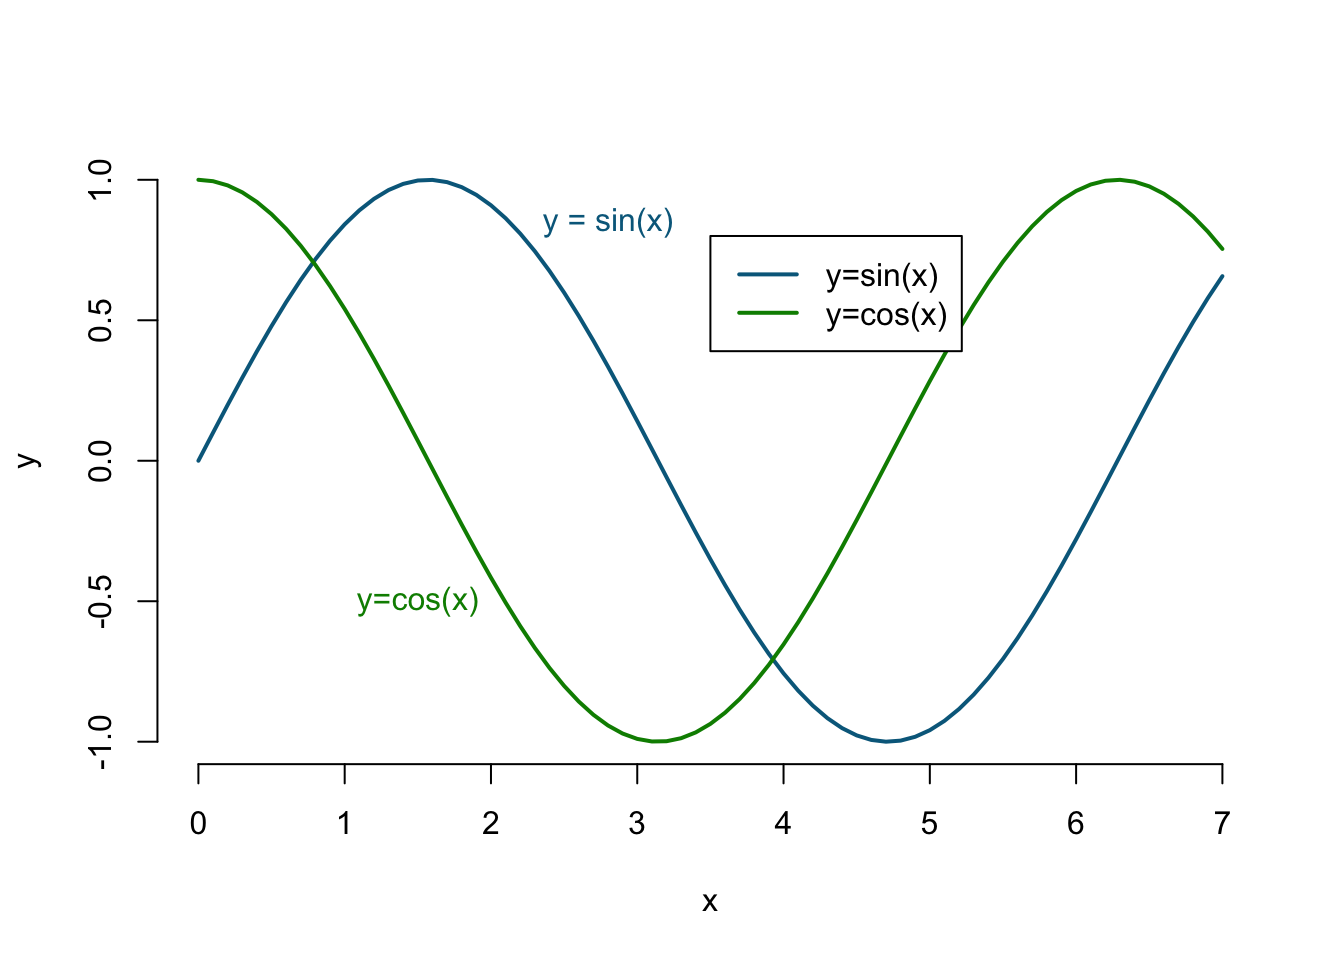
\includegraphics{index_files/figure-latex/unnamed-chunk-3-1.pdf}

When working with data frames, ggplot may seem more attractive and easy
to use than base R functions, simply because many steps are automated.
You may want to try color-coding the different points according to the
varibale class, just as we did before. Then try to add a legend (look up
the function \emph{legend} in the R help). You will find out that it may
be a bit tedious to put all this things together. However, it also gives
you a lot of control about the final looks of your figure once you have
figured out what you want and how you get it. Another advantge of base R
functions is that you are not restircted to the data frame format, which
often makes things easier. For instance, consider this plot:

\begin{Shaded}
\begin{Highlighting}[]
\NormalTok{x=}\KeywordTok{seq}\NormalTok{(}\DecValTok{0}\NormalTok{,}\DecValTok{7}\NormalTok{,}\DataTypeTok{by=}\FloatTok{0.1}\NormalTok{)   }
\CommentTok{# x = (0,0.1,0.2,0.3, ??? ,6.9,7)}
\NormalTok{y=}\KeywordTok{sin}\NormalTok{(x)}


\KeywordTok{plot}\NormalTok{(x,y,}\DataTypeTok{lwd=}\DecValTok{2}\NormalTok{,}\DataTypeTok{type=}\StringTok{"l"}\NormalTok{,}\DataTypeTok{col=}\StringTok{"deepskyblue4"}\NormalTok{,}\DataTypeTok{axes=}\OtherTok{FALSE}\NormalTok{) }
\CommentTok{#plot without axes}

\KeywordTok{axis}\NormalTok{(}\DecValTok{1}\NormalTok{) }\CommentTok{#add axes to plot}
\KeywordTok{axis}\NormalTok{(}\DecValTok{2}\NormalTok{)}

\KeywordTok{text}\NormalTok{(}\FloatTok{2.8}\NormalTok{,}\FloatTok{0.85}\NormalTok{,}\StringTok{"y = sin(x)"}\NormalTok{,}\DataTypeTok{col=}\StringTok{"deepskyblue4"}\NormalTok{)   }
\CommentTok{# add some text at coordinates x = 2.8, y = 0.85}

\KeywordTok{lines}\NormalTok{(x,}\KeywordTok{cos}\NormalTok{(x),}\DataTypeTok{lwd=}\DecValTok{2}\NormalTok{,}\DataTypeTok{col=}\StringTok{"green4"}\NormalTok{)  }\CommentTok{# add a cosine plot ???}
\KeywordTok{text}\NormalTok{(}\FloatTok{1.5}\NormalTok{,}\OperatorTok{-}\FloatTok{0.5}\NormalTok{,}\StringTok{"y=cos(x)"}\NormalTok{,}\DataTypeTok{col=}\StringTok{"green4"}\NormalTok{)   }\CommentTok{# ??? and label it}

\KeywordTok{legend}\NormalTok{(}\FloatTok{3.5}\NormalTok{,}\FloatTok{0.8}\NormalTok{,}\DataTypeTok{legend=}\KeywordTok{c}\NormalTok{(}\StringTok{"y=sin(x)"}\NormalTok{,}\StringTok{"y=cos(x)"}\NormalTok{),}
\DataTypeTok{col=}\KeywordTok{c}\NormalTok{(}\StringTok{"deepskyblue4"}\NormalTok{,}\StringTok{"green4"}\NormalTok{),}\DataTypeTok{lwd=}\DecValTok{2}\NormalTok{)   }
\end{Highlighting}
\end{Shaded}

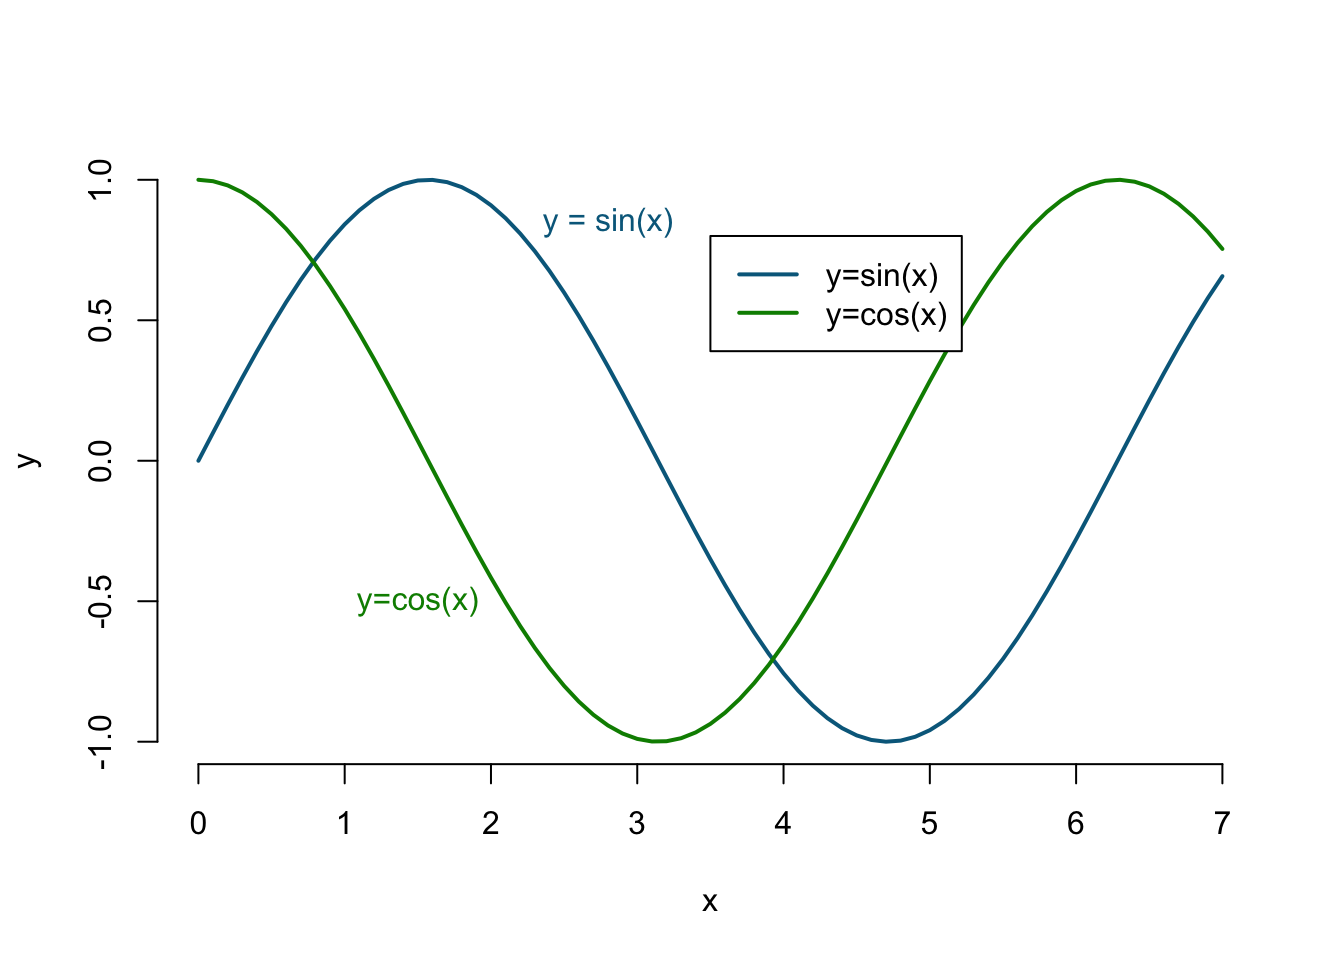
\includegraphics{index_files/figure-latex/unnamed-chunk-4-1.pdf}

\begin{Shaded}
\begin{Highlighting}[]
\CommentTok{# add a legend to the plot}
\end{Highlighting}
\end{Shaded}

Instead of using a data frame, we have created vectors of variables and
used them in several different ways. You will explore this more in the
exercise sessions.

By now you should see that R is very versatile and can be used for much
more than simply doing statistics. This course will teach you the basics
of R so that you can start using it for your research projects. An
essential part is that you should also learn how to find and use
additional resources, such as the help function in R, books, the
internet, etc. Nobody knows all of R - it is an ever growing community
endevaour and looking up how things work, which functions or packages
are available, or how other people solved a problem is an essential part
of learning to be proficient in R.

\hypertarget{working-with-data-frames}{%
\section{Working with data frames}\label{working-with-data-frames}}

\hypertarget{loading-datasets}{%
\subsection{Loading datasets}\label{loading-datasets}}

How to we feed R our data? Of course, we can just type it into the
console, a bit like in the previous base R graphics example. For large
data sets (or rather anythign that is not an eytremely small data set)
this is not practical. We want to load our data from a file, which makes
our analysis easily reproducible if we share data and R scripts with
someone. First we need to make sure R knows where our working directory
is, using the function \emph{setwd} (set working directory):

\begin{Shaded}
\begin{Highlighting}[]
\KeywordTok{setwd}\NormalTok{(}\StringTok{"/Users/stephan/Dropbox/Teaching/StatisticsForBiology/"}\NormalTok{)}
\end{Highlighting}
\end{Shaded}

If you want to check your current working directory, you can do this
with \emph{getwd()}.

I use a dataset about the number of plates on sticklebacks. You can find
this dataset (and many others) on ilias. We can load a dataset using the
function \emph{read.csv} and store it in the variable stickleback

\begin{Shaded}
\begin{Highlighting}[]
\NormalTok{stickleback =}\StringTok{ }\KeywordTok{read.csv}\NormalTok{(}\StringTok{"chap03e3SticklebackPlates.csv"}\NormalTok{)}
\end{Highlighting}
\end{Shaded}

The variable \emph{stickleback} now contains a so called data frame. We
can have a quick summary of the content of this data frame using the
command \emph{str} (short for \emph{STR}ucture):

\begin{Shaded}
\begin{Highlighting}[]
\KeywordTok{str}\NormalTok{(stickleback)}
\end{Highlighting}
\end{Shaded}

\begin{verbatim}
## 'data.frame':    344 obs. of  3 variables:
##  $ id      : Factor w/ 344 levels "4-1","4-10","4-100",..: 1 102 282 293 2 22 42 131 212 280 ...
##  $ plates  : int  11 63 22 10 14 11 58 36 31 61 ...
##  $ genotype: Factor w/ 3 levels "MM","Mm","mm": 3 2 2 2 3 3 2 2 2 2 ...
\end{verbatim}

We can see form the output that we have 344 observations (= sample size)
and for each individual we have measured 3 variables (id, plates and
genotypes). ID and genotpye are so-called factors, that is, a
catergorical variable and plates is of type integer.

We used the function \emph{read.csv} because our data is stored in the
CSV format (short for \emph{c}omma \emph{s}eperated \emph{v}alues - open
the file in a text editor to see what that means). CSV is a common
format and you can export your data from software like Excel in that
format. Of course, R provides functions for other formats as well or you
an use the read.table() function where you can specify how the data
should be read and transformed into a data frame.

Let us use our ggplot skills to create a nice figure that visualizes our
data set. For this we introduce the fucntion \emph{geom\_bar()} which
allows us to make a bar plot of the number of plates per indivudal,
colored by genotype:

\begin{Shaded}
\begin{Highlighting}[]
\KeywordTok{ggplot}\NormalTok{(}\DataTypeTok{data =}\NormalTok{ stickleback) }\OperatorTok{+}\StringTok{ }
\StringTok{  }\KeywordTok{geom_bar}\NormalTok{(}\DataTypeTok{mapping =} \KeywordTok{aes}\NormalTok{(}\DataTypeTok{x =}\NormalTok{ plates,}\DataTypeTok{color=}\NormalTok{genotype)) }\OperatorTok{+}\StringTok{ }
\StringTok{  }\KeywordTok{theme_classic}\NormalTok{()}
\end{Highlighting}
\end{Shaded}

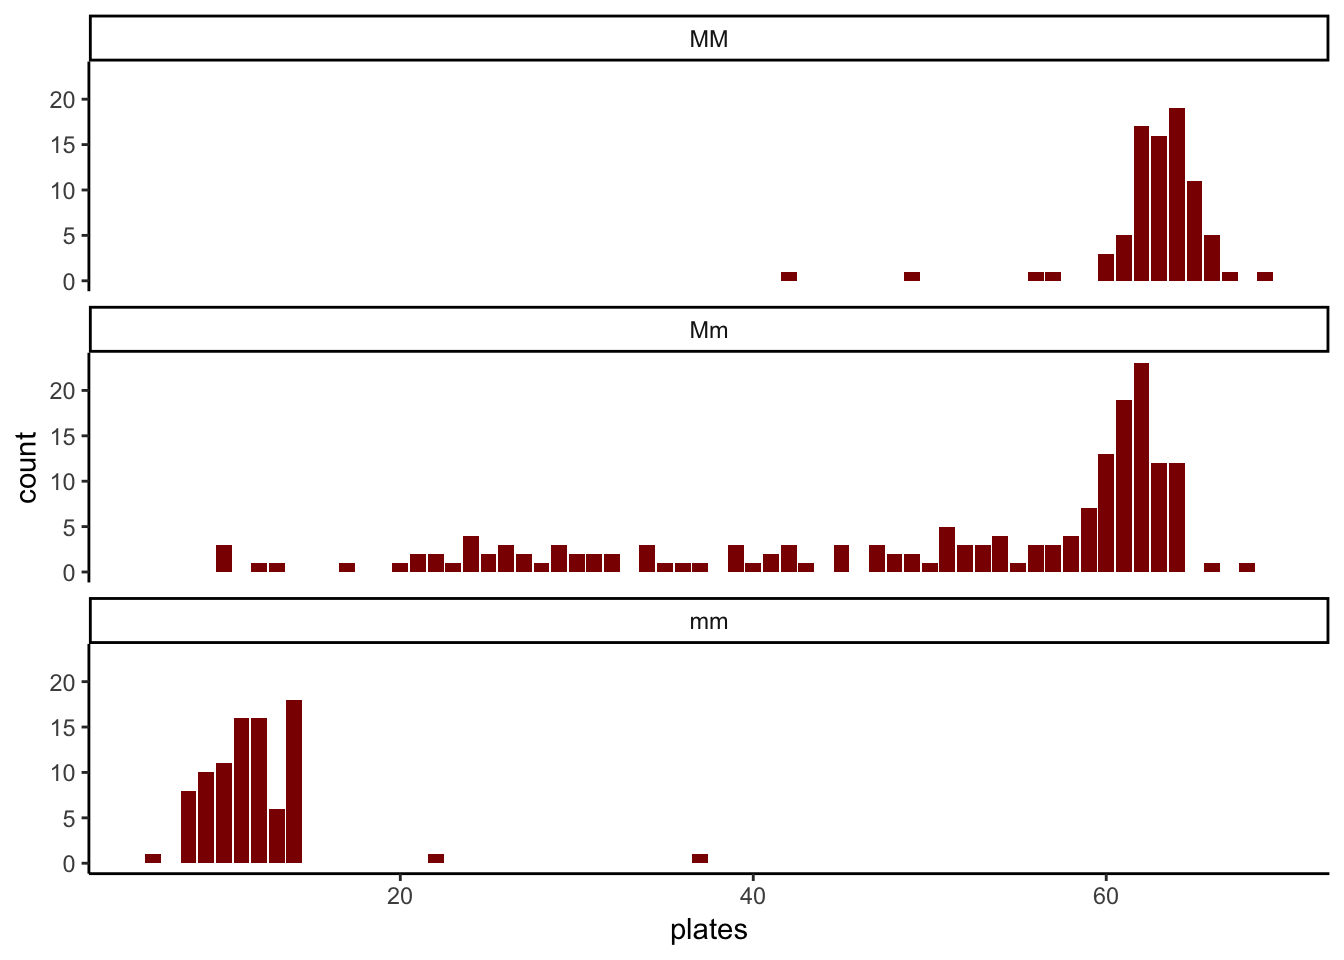
\includegraphics{index_files/figure-latex/unnamed-chunk-8-1.pdf}

This figure is a bit messy. A better way would be to show the
distribution for each genotype in its own window. This can be done using
the function \emph{facet\_wrap}. As before, we can simply add this to
our ggplot command:

\begin{Shaded}
\begin{Highlighting}[]
\KeywordTok{ggplot}\NormalTok{(}\DataTypeTok{data =}\NormalTok{ stickleback) }\OperatorTok{+}\StringTok{ }
\StringTok{  }\KeywordTok{geom_bar}\NormalTok{(}\DataTypeTok{mapping =} \KeywordTok{aes}\NormalTok{(}\DataTypeTok{x =}\NormalTok{ plates),}\DataTypeTok{fill=}\StringTok{"darkred"}\NormalTok{) }\OperatorTok{+}\StringTok{ }
\StringTok{  }\KeywordTok{facet_wrap}\NormalTok{(}\OperatorTok{~}\NormalTok{genotype,}\DataTypeTok{nrow =} \DecValTok{3}\NormalTok{) }\OperatorTok{+}
\StringTok{  }\KeywordTok{theme_classic}\NormalTok{()}
\end{Highlighting}
\end{Shaded}

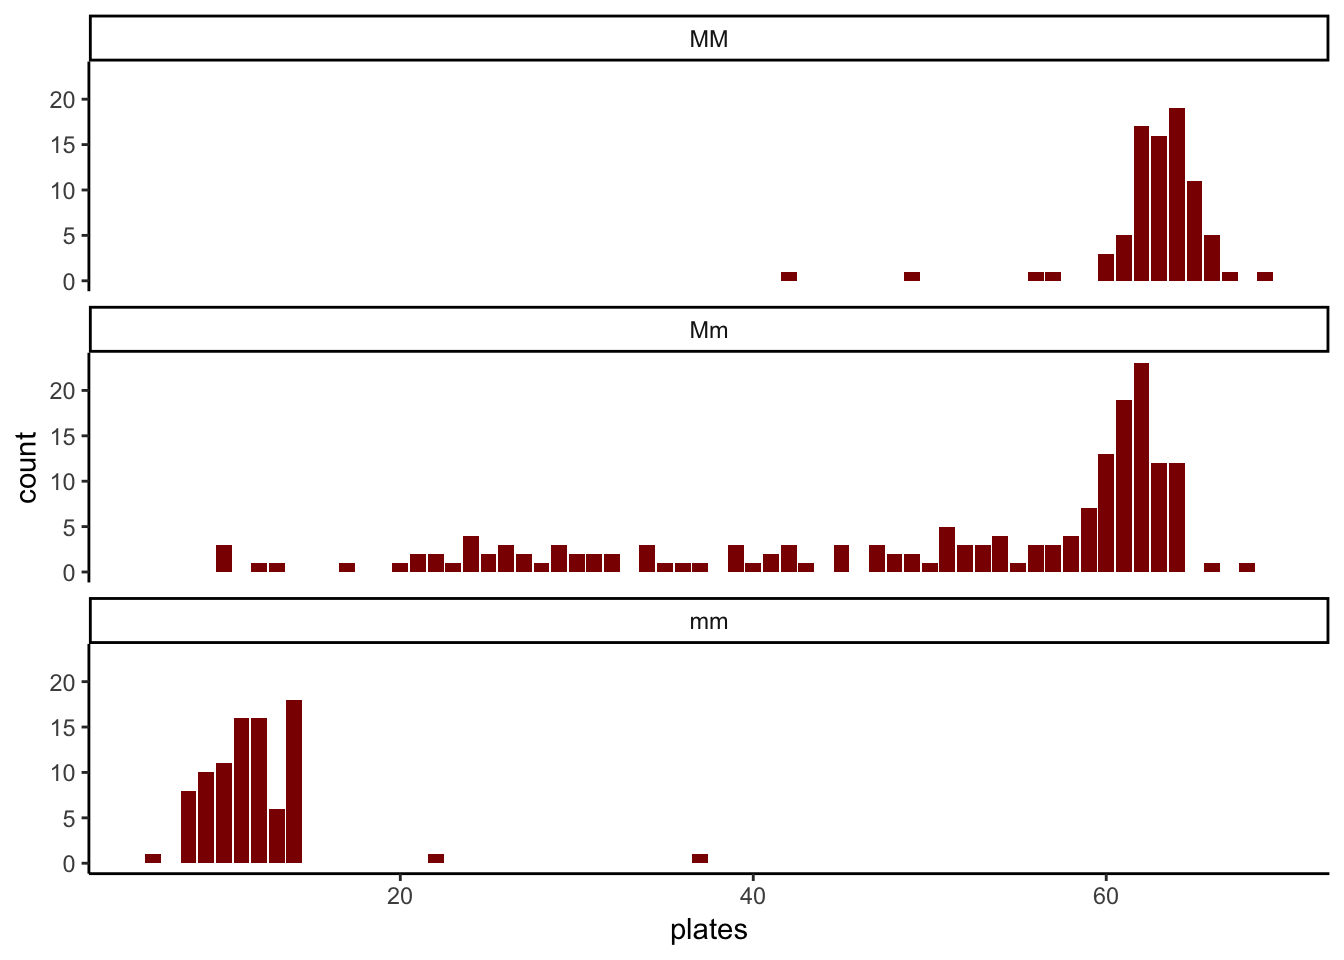
\includegraphics{index_files/figure-latex/unnamed-chunk-9-1.pdf}

We used a new symbol here: the \textasciitilde{}. This is part of an R
object called formula and it will alter become clear why we used it here
like this. For now, just remember to use it in front of the varibale
name in facet wrap. The second aprameter is simply the number of rows in
the plot. Try changing it and see what happens. Note: the variable that
you pass to facet\_wrap shoudl \textbf{always} be categorical!

\hypertarget{manipulating-data-frames}{%
\subsection{Manipulating data frames}\label{manipulating-data-frames}}

A data frame is essentially a spreadsheet or a table (or rather a
matrix). Therfore, we acess each column or each row, if we want to. This
can be done using the \emph{{[},{]}} symbols. The element in row 3 and
column 5 is given by:

\begin{Shaded}
\begin{Highlighting}[]
\NormalTok{stickleback[}\DecValTok{3}\NormalTok{,}\DecValTok{5}\NormalTok{]}
\end{Highlighting}
\end{Shaded}

\begin{verbatim}
## NULL
\end{verbatim}

the whole 3rd column can be accesses by

\begin{Shaded}
\begin{Highlighting}[]
\NormalTok{stickleback[,}\DecValTok{3}\NormalTok{]}
\end{Highlighting}
\end{Shaded}

\begin{verbatim}
##   [1] mm Mm Mm Mm mm mm Mm Mm Mm Mm Mm mm mm mm Mm Mm mm Mm Mm MM Mm Mm mm
##  [24] Mm MM Mm mm MM Mm Mm MM mm Mm Mm mm Mm mm MM Mm mm Mm MM mm Mm Mm MM
##  [47] Mm mm mm Mm Mm MM mm mm mm Mm MM MM Mm MM MM Mm MM Mm mm mm MM Mm Mm
##  [70] MM MM Mm MM Mm MM MM Mm Mm Mm mm Mm Mm Mm Mm MM Mm Mm Mm Mm MM mm Mm
##  [93] Mm mm MM Mm mm MM mm mm Mm mm mm Mm MM Mm mm mm Mm Mm MM MM Mm mm Mm
## [116] MM MM Mm mm Mm Mm MM mm MM mm mm Mm Mm Mm mm Mm mm Mm mm Mm MM Mm Mm
## [139] Mm Mm MM Mm MM Mm Mm Mm mm MM Mm MM MM MM Mm Mm mm mm Mm MM MM Mm Mm
## [162] mm Mm Mm mm Mm mm Mm Mm MM Mm MM Mm MM MM Mm mm MM mm Mm Mm Mm Mm Mm
## [185] Mm Mm mm Mm MM Mm Mm MM mm MM Mm mm Mm Mm Mm Mm Mm Mm Mm Mm Mm Mm MM
## [208] MM Mm Mm mm Mm mm mm Mm MM Mm Mm Mm Mm mm mm Mm Mm Mm mm MM MM MM Mm
## [231] Mm mm MM MM MM MM Mm Mm MM Mm MM mm mm Mm Mm Mm MM mm mm MM mm Mm MM
## [254] Mm Mm mm mm Mm Mm MM mm Mm Mm mm Mm Mm Mm Mm mm MM Mm mm Mm MM Mm mm
## [277] Mm Mm MM mm mm Mm MM Mm Mm mm MM mm Mm Mm Mm MM mm MM Mm Mm mm MM MM
## [300] mm MM MM MM Mm Mm MM mm mm MM MM mm Mm Mm Mm Mm MM mm Mm Mm Mm Mm MM
## [323] Mm mm Mm Mm Mm Mm Mm Mm mm MM mm mm Mm Mm Mm mm Mm mm MM mm Mm mm
## Levels: MM Mm mm
\end{verbatim}

and the 5th row by

\begin{Shaded}
\begin{Highlighting}[]
\NormalTok{stickleback[}\DecValTok{5}\NormalTok{,]}
\end{Highlighting}
\end{Shaded}

\begin{verbatim}
##     id plates genotype
## 5 4-10     14       mm
\end{verbatim}

Note that stickleback{[}{[},3{]}{]} gives you all measurment of the 3rd
variable in our dataframe and is hence equivalent to
stickleback\$genotype. The vector stickleback{[}5,{]} on the other hand
gives you a vector with the 3 measured values of the 5 th individual.

We can also use this way of accessing elements to find elements of a
certain type, for instance, fi we want to know the genotype of all
individuals with more then 30 plates, we can get this in the following
way:

\begin{Shaded}
\begin{Highlighting}[]
\NormalTok{stickleback[stickleback}\OperatorTok{$}\NormalTok{plates}\OperatorTok{>}\DecValTok{20}\NormalTok{,}\DecValTok{3}\NormalTok{]}
\end{Highlighting}
\end{Shaded}

Try to understand what is happening here by teasing apart and
investigating the differnt parts of this (nested) command. What would
happen if you removed the \emph{stickleback\$plates\textgreater{}20}
from the command, or the \emph{3}.

A slightly more elegant way to get this is by using the function
\emph{filter} (make sure you have the package dyplr loaded!):

\begin{Shaded}
\begin{Highlighting}[]
\KeywordTok{filter}\NormalTok{(stickleback,plates}\OperatorTok{>}\DecValTok{20}\NormalTok{)}
\end{Highlighting}
\end{Shaded}

which gives ou a data frame with only the individuals that satisfy the
condition set in the argument.

\hypertarget{adding-variables-to-data-frames}{%
\subsection{Adding variables to data
frames}\label{adding-variables-to-data-frames}}

Sometimes we wish to extend our dataframe with calcualtions we did
during our analysis or with additional measurements. This can be done
with the function \emph{mutate()}. It simply adds new columns at the end
of your dataset. Let's say we want to identify which indivduals have
fewer or more plates as comapred to the global mean:

\begin{Shaded}
\begin{Highlighting}[]
\NormalTok{diff.to.mean =}\StringTok{ }\NormalTok{stickleback}\OperatorTok{$}\NormalTok{plates }\OperatorTok{-}\StringTok{ }\KeywordTok{mean}\NormalTok{(stickleback}\OperatorTok{$}\NormalTok{plates)}
\NormalTok{stickleback2 =}\StringTok{ }\KeywordTok{mutate}\NormalTok{(stickleback,}\DataTypeTok{difference =}\NormalTok{ diff.to.mean)}
\KeywordTok{head}\NormalTok{(stickleback2)}
\end{Highlighting}
\end{Shaded}

\begin{verbatim}
##     id plates genotype difference
## 1  4-1     11       mm  -32.43314
## 2  4-2     63       Mm   19.56686
## 3  4-4     22       Mm  -21.43314
## 4  4-5     10       Mm  -33.43314
## 5 4-10     14       mm  -29.43314
## 6 4-12     11       mm  -32.43314
\end{verbatim}

\hypertarget{subsetting-a-data-frame}{%
\subsection{Subsetting a data frame}\label{subsetting-a-data-frame}}

We have alreaddy seen how to look at a subset of your data frame using
indexing. Here is another slightly more elegant way of doing this,
especially when many conditions are combined over multiple variables.
For instance, what if we want to consider only stickleback with more
than 20 plates:

\begin{Shaded}
\begin{Highlighting}[]
\KeywordTok{head}\NormalTok{(}\KeywordTok{subset}\NormalTok{(stickleback, plates}\OperatorTok{>}\DecValTok{20}\NormalTok{))}
\end{Highlighting}
\end{Shaded}

\begin{verbatim}
##      id plates genotype
## 2   4-2     63       Mm
## 3   4-4     22       Mm
## 7  4-14     58       Mm
## 8  4-23     36       Mm
## 9  4-31     31       Mm
## 10 4-38     61       Mm
\end{verbatim}

We could now compare how the disitrbution of genotpyes changes if we
condition on more than 10 plates:

\begin{Shaded}
\begin{Highlighting}[]
\KeywordTok{ggplot}\NormalTok{(}\DataTypeTok{data =} \KeywordTok{subset}\NormalTok{(stickleback, plates}\OperatorTok{>}\DecValTok{20}\NormalTok{)) }\OperatorTok{+}\StringTok{ }
\StringTok{  }\KeywordTok{geom_bar}\NormalTok{(}\DataTypeTok{mapping=} \KeywordTok{aes}\NormalTok{(}\DataTypeTok{x =}\NormalTok{ genotype)) }\OperatorTok{+}
\StringTok{  }\KeywordTok{labs}\NormalTok{(}\DataTypeTok{title=}\StringTok{"Stickleback with more than 20 plates"}\NormalTok{,}
        \DataTypeTok{x =}\StringTok{"Genotype"}\NormalTok{, }\DataTypeTok{y =} \StringTok{"Count"}\NormalTok{)}
\end{Highlighting}
\end{Shaded}

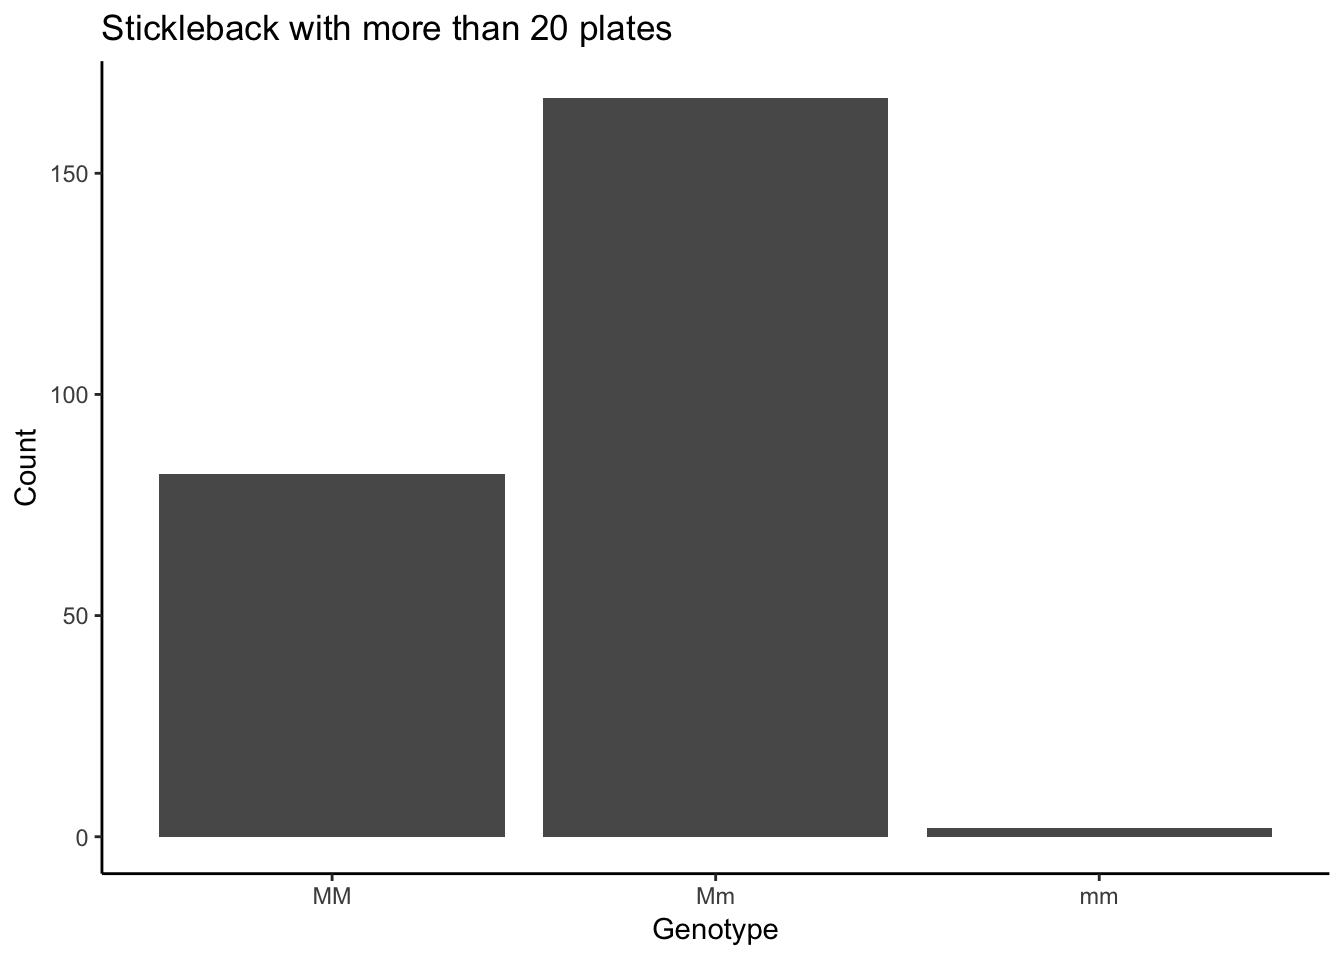
\includegraphics{index_files/figure-latex/unnamed-chunk-17-1.pdf}

\begin{Shaded}
\begin{Highlighting}[]
\KeywordTok{ggplot}\NormalTok{(}\DataTypeTok{data =}\NormalTok{ stickleback) }\OperatorTok{+}\StringTok{ }
\StringTok{  }\KeywordTok{geom_bar}\NormalTok{(}\DataTypeTok{mapping=} \KeywordTok{aes}\NormalTok{(}\DataTypeTok{x =}\NormalTok{ genotype)) }\OperatorTok{+}
\StringTok{  }\KeywordTok{labs}\NormalTok{(}\DataTypeTok{title=}\StringTok{"All Stickleback"}\NormalTok{,}
        \DataTypeTok{x =}\StringTok{"Genotype"}\NormalTok{, }\DataTypeTok{y =} \StringTok{"Count"}\NormalTok{)}
\end{Highlighting}
\end{Shaded}

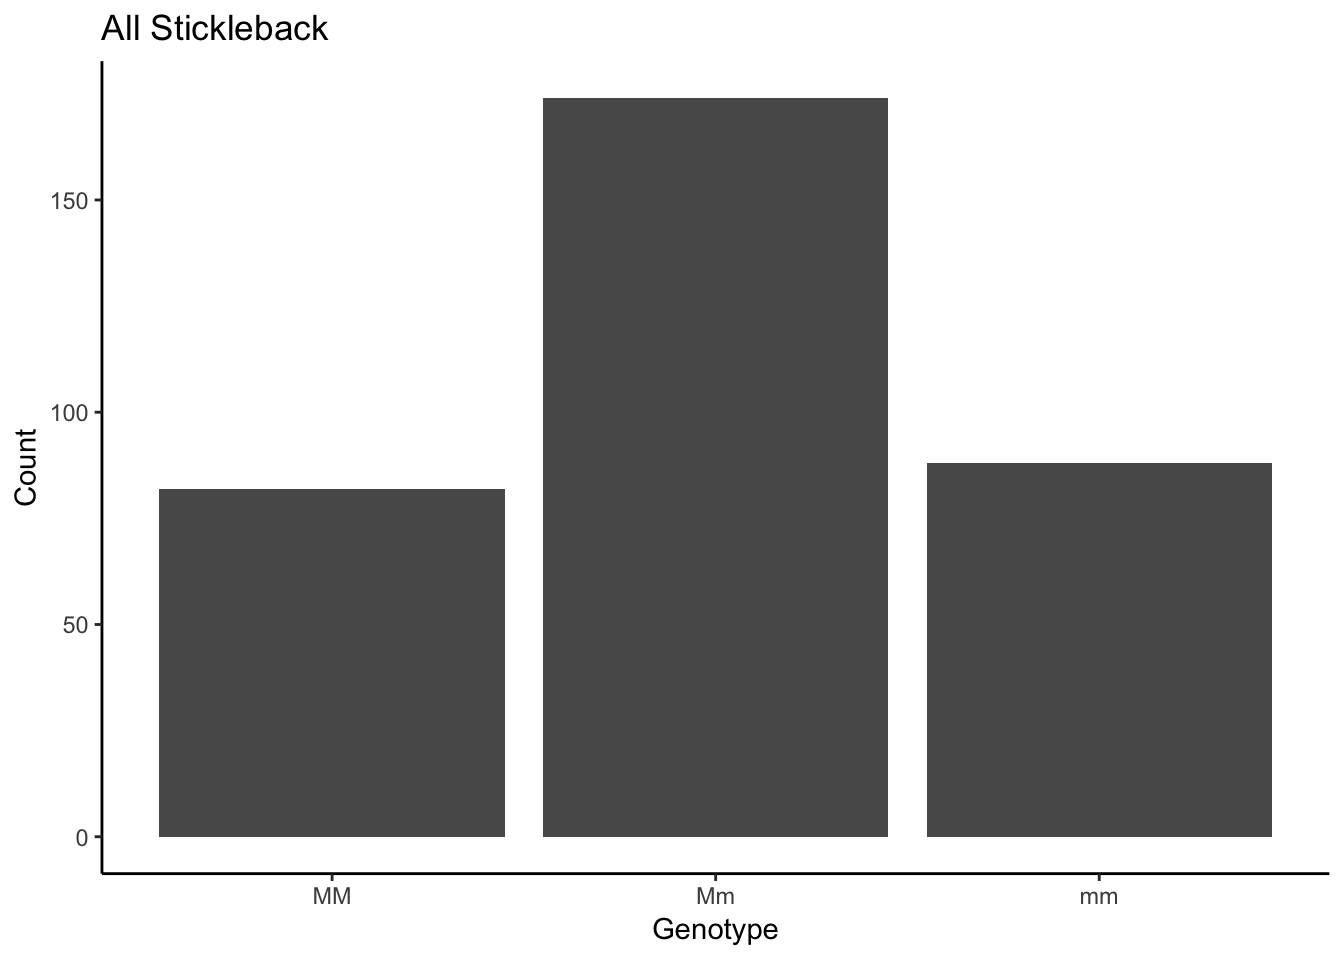
\includegraphics{index_files/figure-latex/unnamed-chunk-17-2.pdf} There
are a few \emph{mm} genotypes with more than 20 plates. But how many?

\begin{Shaded}
\begin{Highlighting}[]
\KeywordTok{subset}\NormalTok{(stickleback,plates }\OperatorTok{>}\StringTok{ }\DecValTok{20} \OperatorTok{&}\StringTok{ }\NormalTok{genotype }\OperatorTok{==}\StringTok{ "mm"}\NormalTok{)}
\end{Highlighting}
\end{Shaded}

\begin{verbatim}
##       id plates genotype
## 100 4-25     37       mm
## 132 4-87     22       mm
\end{verbatim}

It turns out there are exactly two: one with 37 plates and one with 22.
We have used logical operators here: ``\&'' means that both conditions
need to be satisfied. In contrast, try to see what the symbol
``\textbar{}'' means:

\begin{Shaded}
\begin{Highlighting}[]
\KeywordTok{head}\NormalTok{(}\KeywordTok{subset}\NormalTok{(stickleback,plates }\OperatorTok{>}\StringTok{ }\DecValTok{20} \OperatorTok{|}\StringTok{ }\NormalTok{genotype }\OperatorTok{==}\StringTok{ "mm"}\NormalTok{))}
\end{Highlighting}
\end{Shaded}

\begin{verbatim}
##     id plates genotype
## 1  4-1     11       mm
## 2  4-2     63       Mm
## 3  4-4     22       Mm
## 5 4-10     14       mm
## 6 4-12     11       mm
## 7 4-14     58       Mm
\end{verbatim}

You may have guessed it already, the ``\textbar{}'' represetns the
logical ``or'' command, indicating that either of the two conditions
needs to be satisfied. Note that for logical comparions we use the
``=='' and not the ``='' symbol, which is reserved for assignments. What
is the difference? Try it:

\begin{Shaded}
\begin{Highlighting}[]
\NormalTok{a =}\StringTok{ }\DecValTok{5}

\NormalTok{a }\OperatorTok{==}\StringTok{ }\DecValTok{5}
\end{Highlighting}
\end{Shaded}

\begin{verbatim}
## [1] TRUE
\end{verbatim}

\begin{Shaded}
\begin{Highlighting}[]
\NormalTok{a }\OperatorTok{==}\StringTok{ }\DecValTok{6}
\end{Highlighting}
\end{Shaded}

\begin{verbatim}
## [1] FALSE
\end{verbatim}

We can also use the symbols \textless{} (smaller), \textgreater{}
(larger), \textless{}= (smaller or equal), \textgreater{}= (larger or
equal), != (not equal) and combine them into logical statements.

\hypertarget{practice-questions}{%
\subsubsection{\texorpdfstring{\emph{Practice
Questions:}}{Practice Questions:}}\label{practice-questions}}

\begin{itemize}
\item
  Add a new varaible to the stickleback data frame that contains the
  difference between plate number and the mean plate number for that
  individuals genotype.
\item
  Load the flights dataset:
\end{itemize}

\begin{Shaded}
\begin{Highlighting}[]
\KeywordTok{library}\NormalTok{(nycflights13)}
\end{Highlighting}
\end{Shaded}

Find all flights that

\begin{itemize}
\item
  Had an arrival delay of two or more hours
\item
  Flew to Houston (IAH or HOU)
\item
  Were operated by United, American, or Delta
\item
  Departed in summer (July, August, and September)
\item
  Arrived more than two hours late, but didn???t leave late
\item
  Were delayed by at least an hour, but made up over 30 minutes in
  flight
\item
  Departed between midnight and 6am
\end{itemize}

\hypertarget{calculating-descriptive-statistics}{%
\section{Calculating Descriptive
Statistics}\label{calculating-descriptive-statistics}}

We continue using the stickleback data set and calcualte some statistics
on it. A simple way to get a quick overview about the properties of your
data frame is using the funciton \emph{summary}:

\begin{Shaded}
\begin{Highlighting}[]
\KeywordTok{summary}\NormalTok{(stickleback)}
\end{Highlighting}
\end{Shaded}

\begin{verbatim}
##        id          plates      genotype
##  4-1    :  1   Min.   : 6.00   MM: 82  
##  4-10   :  1   1st Qu.:14.00   Mm:174  
##  4-100  :  1   Median :57.00   mm: 88  
##  4-101  :  1   Mean   :43.43           
##  4-103  :  1   3rd Qu.:62.00           
##  4-105  :  1   Max.   :69.00           
##  (Other):338
\end{verbatim}

If you want to calcualte a specific statistic, like the mean of a
variable, this can be done easily:

\begin{Shaded}
\begin{Highlighting}[]
\KeywordTok{mean}\NormalTok{(stickleback}\OperatorTok{$}\NormalTok{plates)}
\end{Highlighting}
\end{Shaded}

\begin{verbatim}
## [1] 43.43314
\end{verbatim}

You may have noticed that we have no calcualted the mean number of
plates for \emph{ALL} fish in our data set. What if we want to calcualte
the number of plates for a specific genotype? We can use the function
filter:

\begin{Shaded}
\begin{Highlighting}[]
\NormalTok{stickleback.mm =}\StringTok{ }\KeywordTok{filter}\NormalTok{(stickleback,genotype}\OperatorTok{==}\StringTok{"mm"}\NormalTok{)}
\KeywordTok{mean}\NormalTok{(stickleback.mm}\OperatorTok{$}\NormalTok{plates)}
\end{Highlighting}
\end{Shaded}

\begin{verbatim}
## [1] 11.67045
\end{verbatim}

You could now calcualte the mean plate numbers for each genotpye in this
way:

\begin{Shaded}
\begin{Highlighting}[]
\NormalTok{mean.mm =}\StringTok{ }\KeywordTok{mean}\NormalTok{((}\KeywordTok{filter}\NormalTok{(stickleback,genotype}\OperatorTok{==}\StringTok{"mm"}\NormalTok{))}\OperatorTok{$}\NormalTok{plates)}
\NormalTok{mean.mM =}\StringTok{ }\KeywordTok{mean}\NormalTok{((}\KeywordTok{filter}\NormalTok{(stickleback,genotype}\OperatorTok{==}\StringTok{"mM"}\NormalTok{))}\OperatorTok{$}\NormalTok{plates)}
\NormalTok{mean.MM =}\StringTok{ }\KeywordTok{mean}\NormalTok{((}\KeywordTok{filter}\NormalTok{(stickleback,genotype}\OperatorTok{==}\StringTok{"MM"}\NormalTok{))}\OperatorTok{$}\NormalTok{plates)}
\end{Highlighting}
\end{Shaded}

\textbf{Note:} The tidyverse offers an elegant way to write a long
series of commands in a very readable format. To show you how to combine
multiple commands quickly, we first need two more functions,
\emph{group\_by} and \emph{summarize}, and a new operator called the
pipe: \%\textgreater{}\% (because we create a pipeline thorugh which our
data ``flows''). The above code to calculate the mean for each genotype
would become:

\begin{Shaded}
\begin{Highlighting}[]
\NormalTok{stickleback }\OperatorTok\StringTok{ }
\KeywordTok{group_by}\NormalTok{(genotype) }\OperatorTok
\KeywordTok{summarise}\NormalTok{(}\DataTypeTok{avg =} \KeywordTok{mean}\NormalTok{(plates))}
\end{Highlighting}
\end{Shaded}

\begin{verbatim}
##        avg
## 1 43.43314
\end{verbatim}

This is very readable: you take the dataframe stickleback, group it by
genotye and summarize it by calcualting the mean number of plates.
However, errors might be more difficutl to spot when the code is written
in that way, as intermediate steps cannot be checked.

In the exercises you will learn a few more useful functions to
rearrange, filter, extend and edit data frames.

\emph{Practice Question:} Can you come up with anotehr way to do this
whithout using filter?

\emph{Two possible answers (there are many ways to do this):}
Straightforward ``indexing'':

\begin{Shaded}
\begin{Highlighting}[]
\NormalTok{mean.mm =}\StringTok{ }\KeywordTok{mean}\NormalTok{(stickleback}\OperatorTok{$}\NormalTok{plates[stickleback}\OperatorTok{$}\NormalTok{genotype}\OperatorTok{==}\StringTok{"mm"}\NormalTok{])}
\NormalTok{mean.mM =}\StringTok{ }\KeywordTok{mean}\NormalTok{(stickleback}\OperatorTok{$}\NormalTok{plates[stickleback}\OperatorTok{$}\NormalTok{genotype}\OperatorTok{==}\StringTok{"mM"}\NormalTok{])}
\NormalTok{mean.MM =}\StringTok{ }\KeywordTok{mean}\NormalTok{(stickleback}\OperatorTok{$}\NormalTok{plates[stickleback}\OperatorTok{$}\NormalTok{genotype}\OperatorTok{==}\StringTok{"MM"}\NormalTok{])}
\end{Highlighting}
\end{Shaded}

or by using the function \emph{tapply} (look up the help page for this
function by typing ``?tapply''):

\begin{Shaded}
\begin{Highlighting}[]
\NormalTok{mean.plates =}\StringTok{ }\KeywordTok{tapply}\NormalTok{(stickleback}\OperatorTok{$}\NormalTok{plates,stickleback}\OperatorTok{$}\NormalTok{genotyp,mean)}
\end{Highlighting}
\end{Shaded}

\hypertarget{plots}{%
\subsection{Plots}\label{plots}}

We can do a boxplot easily using ggplot:

\begin{Shaded}
\begin{Highlighting}[]
\KeywordTok{ggplot}\NormalTok{(}\DataTypeTok{data =}\NormalTok{ stickleback) }\OperatorTok{+}\StringTok{ }
\StringTok{  }\KeywordTok{geom_boxplot}\NormalTok{(}\DataTypeTok{mapping =} \KeywordTok{aes}\NormalTok{(}\DataTypeTok{x =}\NormalTok{ genotype, }\DataTypeTok{y =}\NormalTok{ plates))}
\end{Highlighting}
\end{Shaded}

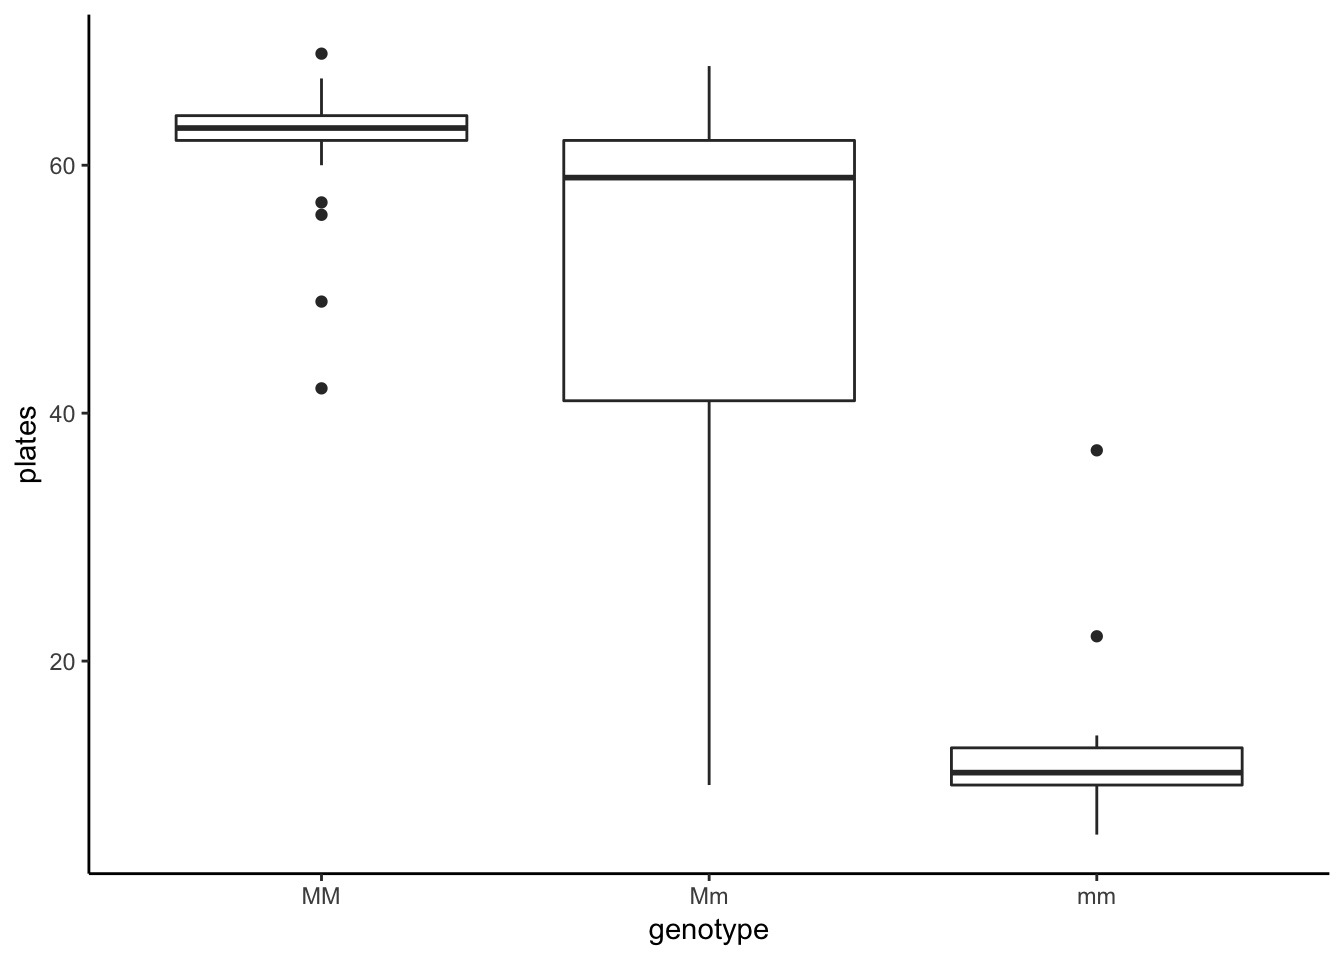
\includegraphics{index_files/figure-latex/unnamed-chunk-29-1.pdf}

In base R, this can be done as well:

\begin{Shaded}
\begin{Highlighting}[]
\KeywordTok{boxplot}\NormalTok{(stickleback}\OperatorTok{$}\NormalTok{plates[stickleback}\OperatorTok{$}\NormalTok{genotype}\OperatorTok{==}\StringTok{"MM"}\NormalTok{],}
\NormalTok{        stickleback}\OperatorTok{$}\NormalTok{plates[stickleback}\OperatorTok{$}\NormalTok{genotype}\OperatorTok{==}\StringTok{"Mm"}\NormalTok{],}
\NormalTok{        stickleback}\OperatorTok{$}\NormalTok{plates[stickleback}\OperatorTok{$}\NormalTok{genotype}\OperatorTok{==}\StringTok{"mm"}\NormalTok{],}
\DataTypeTok{names =} \KeywordTok{c}\NormalTok{(}\StringTok{"MM"}\NormalTok{,}\StringTok{"Mm"}\NormalTok{,}\StringTok{"mm"}\NormalTok{)}
\NormalTok{)}
\end{Highlighting}
\end{Shaded}

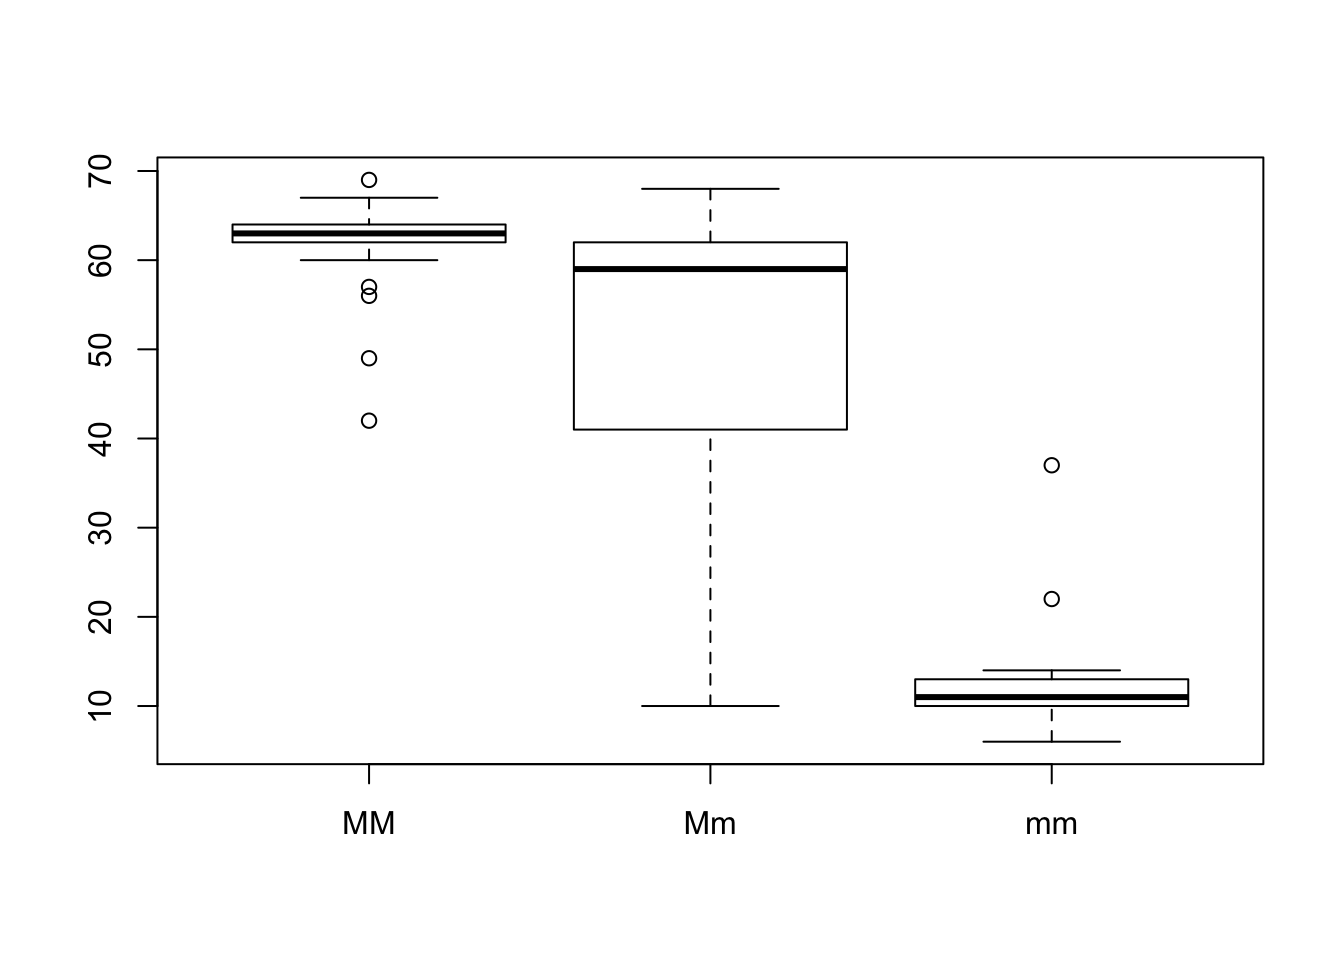
\includegraphics{index_files/figure-latex/unnamed-chunk-30-1.pdf}

\emph{Practice Question:} Can you plot a histogram of plate numbers of
individuals with genotpye mm using base R plotting functions? Hint: Use
what you have learned here and look up the function hist().
Alternatively, use ggplot and geom\_histogram.

\emph{Answer:}

\begin{Shaded}
\begin{Highlighting}[]
\KeywordTok{hist}\NormalTok{(stickleback}\OperatorTok{$}\NormalTok{plates[stickleback}\OperatorTok{$}\NormalTok{genotype}\OperatorTok{==}\StringTok{"mm"}\NormalTok{],}\DataTypeTok{col=}\StringTok{"darkred"}\NormalTok{,}\DataTypeTok{xlab=}\StringTok{"plates"}\NormalTok{,}\DataTypeTok{main=}\StringTok{"Genotype: mm"}\NormalTok{)}
\end{Highlighting}
\end{Shaded}

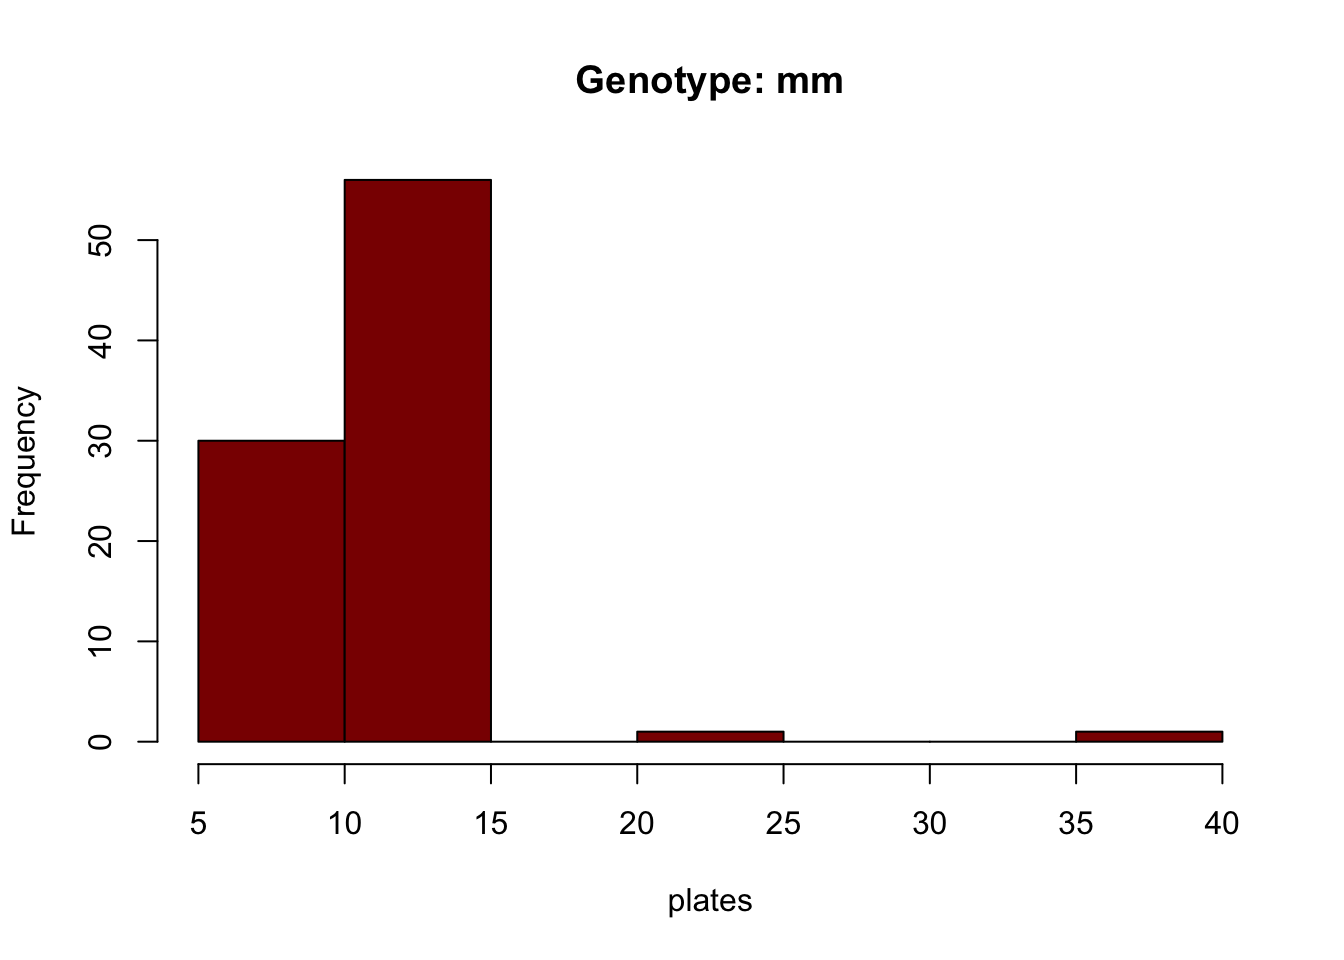
\includegraphics{index_files/figure-latex/unnamed-chunk-31-1.pdf}

\begin{Shaded}
\begin{Highlighting}[]
\KeywordTok{ggplot}\NormalTok{(}\DataTypeTok{data=}\KeywordTok{filter}\NormalTok{(stickleback,genotype }\OperatorTok{==}\StringTok{ "mm"}\NormalTok{)) }\OperatorTok{+}\StringTok{ }
\StringTok{  }\KeywordTok{geom_histogram}\NormalTok{(}\DataTypeTok{mapping =} \KeywordTok{aes}\NormalTok{(}\DataTypeTok{x =}\NormalTok{ plates))}
\end{Highlighting}
\end{Shaded}

\begin{verbatim}
## `stat_bin()` using `bins = 30`. Pick better value with `binwidth`.
\end{verbatim}

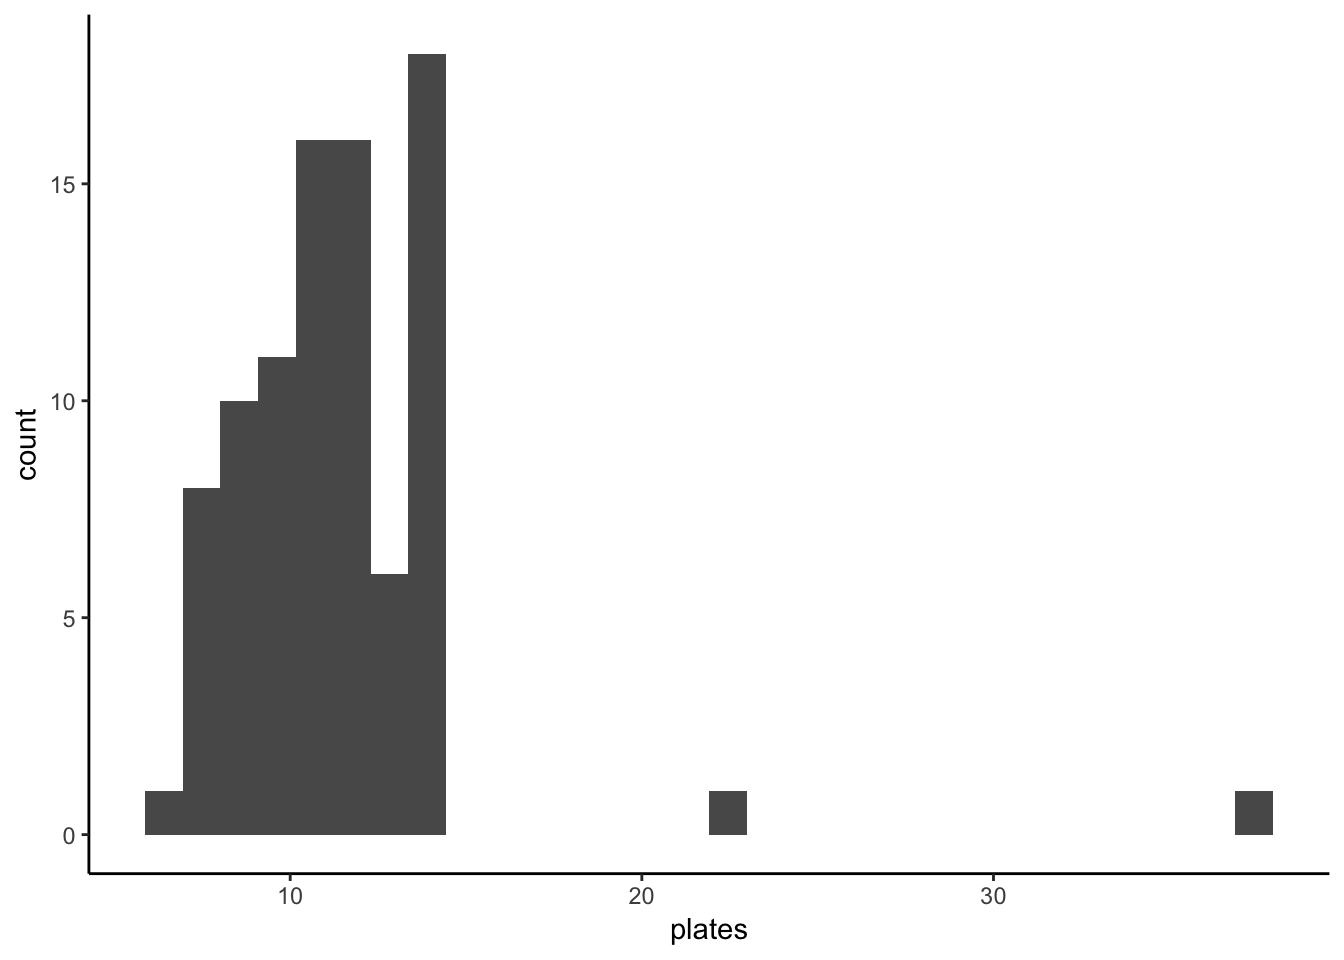
\includegraphics{index_files/figure-latex/unnamed-chunk-31-2.pdf}

\hypertarget{a-bit-of-workflow}{%
\section{A bit of workflow}\label{a-bit-of-workflow}}

In this part you will see how to explore a data set and store your
analysis in a reproducible and reusable way.

\hypertarget{what-is-an-r-script}{%
\subsection{What is an R script}\label{what-is-an-r-script}}

So far we only used the console of R. We enter commands and R executes
them. Most of the time we want to have a whole bunch of commands stored
in a single space: loading the file, preparing and cleaning the
data,make figures, etc. The solution is easy, we jsut store our commands
in a text file with the extension \emph{.R} and tell R do execute this
script. Evene better, RStudio has its own window panel for writing and
executing scripts! Try to open a new R script (via File -\textgreater{}
New -\textgreater{} R script) and just write your code in the newly
opened window. When you have written your code, you can eitehr execute
it step by step by putting the mouse cursor in the line you want to
execute and then hit then \emph{Run} button. If you want to eecute the
whole script from beginning to end, just hit the \emph{Source} button.
This allows you to make reproducible scripts than you can modify and
reuse whenever you need to. This is probably the biggest advantage of R.
Once you have solved a problem and wrote a script for it, you can always
reuse it. The more you use R, the less work will be necessary for each
new project!

In the next part I will introduce the basic tools for creating an
automated analysis that consists of several steps.

\hypertarget{defining-and-using-variables}{%
\subsection{Defining and using
Variables}\label{defining-and-using-variables}}

Defining variables is really easy in R. Unlike in other programming
languages we do not need to precisly define what kind of variable we
want. We can just werite down a name and assign a value, R figures out
the rest. For instance:

\begin{Shaded}
\begin{Highlighting}[]
\NormalTok{x =}\StringTok{ }\DecValTok{5}
\end{Highlighting}
\end{Shaded}

automatically creates a \emph{numeric} variable and assigns the value 5
to it. This command

\begin{Shaded}
\begin{Highlighting}[]
\NormalTok{vec =}\StringTok{ }\KeywordTok{c}\NormalTok{(}\DecValTok{1}\NormalTok{,}\DecValTok{2}\NormalTok{,}\DecValTok{3}\NormalTok{,}\DecValTok{4}\NormalTok{,}\DecValTok{5}\NormalTok{,}\DecValTok{6}\NormalTok{)}
\end{Highlighting}
\end{Shaded}

creates a vectors that contains the values 1 to 6. The \emph{c} here
stands for \emph{concatenate} and tells us to combine all the numbers
into a single vector. You can access the elements of the vector by their
index, e.g., we can set the 5th element of the vector to 0 in the
follwoing way:

\begin{Shaded}
\begin{Highlighting}[]
\NormalTok{vec[}\DecValTok{5}\NormalTok{] =}\StringTok{ }\DecValTok{0} 
\end{Highlighting}
\end{Shaded}

In general it is advised to define the type of a varible before using
it, and also tell R how big this variable will be (that is, how much
memory we need to reserve to store it). For instance, if we want to
define a 3x4 matrix we can use the command \emph{matrix}:

\begin{Shaded}
\begin{Highlighting}[]
\NormalTok{mat=}\KeywordTok{matrix}\NormalTok{(}\DataTypeTok{ncol=}\DecValTok{3}\NormalTok{,}\DataTypeTok{nrow=}\DecValTok{4}\NormalTok{)}
\end{Highlighting}
\end{Shaded}

You can then enter numbers in the rows and columns using the {[}{]}
operator:

\begin{Shaded}
\begin{Highlighting}[]
\NormalTok{mat}
\end{Highlighting}
\end{Shaded}

\begin{verbatim}
##      [,1] [,2] [,3]
## [1,]   NA   NA   NA
## [2,]   NA   NA   NA
## [3,]   NA   NA   NA
## [4,]   NA   NA   NA
\end{verbatim}

\begin{Shaded}
\begin{Highlighting}[]
\NormalTok{mat[}\DecValTok{2}\NormalTok{,}\DecValTok{3}\NormalTok{]=}\StringTok{ }\DecValTok{5} 
\NormalTok{mat}
\end{Highlighting}
\end{Shaded}

\begin{verbatim}
##      [,1] [,2] [,3]
## [1,]   NA   NA   NA
## [2,]   NA   NA    5
## [3,]   NA   NA   NA
## [4,]   NA   NA   NA
\end{verbatim}

You can see that the matrix is intially filled with the object \emph{NA}
which stands for \emph{not available} and ist the term R uses for
missing data. Just like in dataframes (after all a data frame is more or
less a matrix with benefits), you can also name columns and rows and use
them to access the elements:

\begin{Shaded}
\begin{Highlighting}[]
\NormalTok{mat =}\StringTok{ }\KeywordTok{matrix}\NormalTok{(}\DecValTok{1}\OperatorTok{:}\DecValTok{25}\NormalTok{,}\DataTypeTok{nrow=}\DecValTok{5}\NormalTok{,}\DataTypeTok{ncol=}\DecValTok{5}\NormalTok{)}
\KeywordTok{colnames}\NormalTok{(mat) =}\StringTok{ }\KeywordTok{c}\NormalTok{(}\StringTok{"var1"}\NormalTok{,}\StringTok{"var2"}\NormalTok{,}\StringTok{"var3"}\NormalTok{,}\StringTok{"var4"}\NormalTok{,}\StringTok{"var5"}\NormalTok{)}
\KeywordTok{rownames}\NormalTok{(mat) =}\StringTok{ }\KeywordTok{c}\NormalTok{(}\StringTok{"obs1"}\NormalTok{,}\StringTok{"obs2"}\NormalTok{,}\StringTok{"obs3"}\NormalTok{,}\StringTok{"obs4"}\NormalTok{,}\StringTok{"obs5"}\NormalTok{)}
\NormalTok{mat}
\end{Highlighting}
\end{Shaded}

\begin{verbatim}
##      var1 var2 var3 var4 var5
## obs1    1    6   11   16   21
## obs2    2    7   12   17   22
## obs3    3    8   13   18   23
## obs4    4    9   14   19   24
## obs5    5   10   15   20   25
\end{verbatim}

\begin{Shaded}
\begin{Highlighting}[]
\NormalTok{mat[}\StringTok{"obs2"}\NormalTok{,]}
\end{Highlighting}
\end{Shaded}

\begin{verbatim}
## var1 var2 var3 var4 var5 
##    2    7   12   17   22
\end{verbatim}

\begin{Shaded}
\begin{Highlighting}[]
\NormalTok{mat[,}\StringTok{"var3"}\NormalTok{]}
\end{Highlighting}
\end{Shaded}

\begin{verbatim}
## obs1 obs2 obs3 obs4 obs5 
##   11   12   13   14   15
\end{verbatim}

\begin{Shaded}
\begin{Highlighting}[]
\NormalTok{mat[}\StringTok{"obs2"}\NormalTok{,}\StringTok{"var3"}\NormalTok{]}
\end{Highlighting}
\end{Shaded}

\begin{verbatim}
## [1] 12
\end{verbatim}

If we want to store some text, we can write

\begin{Shaded}
\begin{Highlighting}[]
\NormalTok{word =}\StringTok{ "hello"}
\end{Highlighting}
\end{Shaded}

and R will automatically recognize that the string of letters ``hello''
is not numeric and will creat a variable of type \emph{character}. Try
to see how this is different from

\begin{Shaded}
\begin{Highlighting}[]
\NormalTok{letters =}\StringTok{ }\KeywordTok{c}\NormalTok{(}\StringTok{"h"}\NormalTok{,}\StringTok{"e"}\NormalTok{,}\StringTok{"l"}\NormalTok{,}\StringTok{"l"}\NormalTok{,}\StringTok{"o"}\NormalTok{)}
\end{Highlighting}
\end{Shaded}

Next try to see what happens here:

\begin{Shaded}
\begin{Highlighting}[]
\NormalTok{hello =}\StringTok{ }\DecValTok{10}
\NormalTok{word1 =}\StringTok{ "hello"}
\NormalTok{word2 =}\StringTok{ }\NormalTok{hello}
\KeywordTok{print}\NormalTok{(word1)}
\end{Highlighting}
\end{Shaded}

\begin{verbatim}
## [1] "hello"
\end{verbatim}

\begin{Shaded}
\begin{Highlighting}[]
\KeywordTok{print}\NormalTok{(word2)}
\end{Highlighting}
\end{Shaded}

\begin{verbatim}
## [1] 10
\end{verbatim}

\hypertarget{loops}{%
\subsection{Loops}\label{loops}}

Before we have seen how to calcualte the mean number of plates for each
genotype. Essentially we have done the same thing 3 times. Imagine we
woul dhave hundreeds of genotypes. In such situations loops come in
handy. They allow us to automate a process that needs to be repeated
many times. We only introduce the so-called \emph{for-loop} here, which
will allow you to do a lot of things. Once you have understood how it
works, it will be easy to figure out how a \emph{while-loop} works and
what the differences are.

Here is a simple for loop that calcualtes the mean number of plates for
each genotpye in our stickleback data set:

\begin{Shaded}
\begin{Highlighting}[]
\CommentTok{# first we create a vector that contains all genotpyes in our dataset}
\CommentTok{# we can do this manually: }
\CommentTok{# genotypes = c("mm","mM","MM")}
\CommentTok{# or by using the function levels()}
\CommentTok{# that gives us a vector with all the different entries found in a }
\CommentTok{# vector of type factor}

\NormalTok{genotypes =}\StringTok{ }\KeywordTok{levels}\NormalTok{(stickleback}\OperatorTok{$}\NormalTok{genotype)}

\CommentTok{# next, we define a vector that has the same length as the number }
\CommentTok{# of different genotypes and name the elements accordingly}

\NormalTok{plate.numbers =}\StringTok{ }\KeywordTok{vector}\NormalTok{(}\StringTok{"numeric"}\NormalTok{,}\KeywordTok{length}\NormalTok{(genotypes)) }
\KeywordTok{names}\NormalTok{(plate.numbers)=genotypes}

\CommentTok{# no comes the actual loop:}
\ControlFlowTok{for}\NormalTok{(g }\ControlFlowTok{in}\NormalTok{ genotypes)}
\NormalTok{\{}
\NormalTok{  plate.numbers[g]=}\KeywordTok{mean}\NormalTok{(stickleback}\OperatorTok{$}\NormalTok{plates[stickleback}\OperatorTok{$}\NormalTok{genotype}\OperatorTok{==}\NormalTok{g])}
\NormalTok{\}}
\end{Highlighting}
\end{Shaded}

We can see what is happening here by showing the intermediate steps more
explicitly:

\begin{Shaded}
\begin{Highlighting}[]
\NormalTok{i =}\StringTok{ }\DecValTok{1}
\ControlFlowTok{for}\NormalTok{(g }\ControlFlowTok{in}\NormalTok{ genotypes)}
\NormalTok{\{}
  \KeywordTok{print}\NormalTok{(}\KeywordTok{paste}\NormalTok{(}\StringTok{"This is iteration "}\NormalTok{,i,}\StringTok{" of our for-loop"}\NormalTok{))}
  \KeywordTok{print}\NormalTok{(}\KeywordTok{paste}\NormalTok{(}\StringTok{"Genotype "}\NormalTok{,i,}\StringTok{" = "}\NormalTok{,g))}
\NormalTok{  mean.temp =}\StringTok{ }\KeywordTok{mean}\NormalTok{(stickleback}\OperatorTok{$}\NormalTok{plates[stickleback}\OperatorTok{$}\NormalTok{genotype}\OperatorTok{==}\NormalTok{g])}
  \KeywordTok{print}\NormalTok{(}\KeywordTok{paste}\NormalTok{(}\StringTok{"The mean number of plates of genotype "}\NormalTok{,g,}\StringTok{" is "}\NormalTok{,mean.temp))}
\NormalTok{  plate.numbers[g]=mean.temp}
\NormalTok{  i =}\StringTok{ }\NormalTok{i}\OperatorTok{+}\DecValTok{1}
\NormalTok{\}}
\end{Highlighting}
\end{Shaded}

\begin{verbatim}
## [1] "This is iteration  1  of our for-loop"
## [1] "Genotype  1  =  MM"
## [1] "The mean number of plates of genotype  MM  is  62.780487804878"
## [1] "This is iteration  2  of our for-loop"
## [1] "Genotype  2  =  Mm"
## [1] "The mean number of plates of genotype  Mm  is  50.3793103448276"
## [1] "This is iteration  3  of our for-loop"
## [1] "Genotype  3  =  mm"
## [1] "The mean number of plates of genotype  mm  is  11.6704545454545"
\end{verbatim}

There are 3 basics steps here:

\begin{itemize}
\tightlist
\item
  Reserve memory for the output
\item
  Set up how often the loop should be iterated
\item
  The code that should be repeatedly calcualted
\end{itemize}

\emph{Question: Could you come up with an alterantive way to solve this
problem using a loop?}

\hypertarget{if-else}{%
\subsection{If / else}\label{if-else}}

Another useful tool are if/else constructs. They allow you to make
choices during your script. Let us again consider the sticklbeack data
set. Let say we want to calcualte the difference between the number of
plates of plates of an individual and the mean of that indivudal's
genotype. We can do this by combining loops with if/else statements
(admittedly, there are better ways to achieve this but it is a good
instuctive example):

\begin{Shaded}
\begin{Highlighting}[]
\NormalTok{number.obs =}\StringTok{ }\KeywordTok{dim}\NormalTok{(stickleback)[}\DecValTok{1}\NormalTok{]}
\NormalTok{diff.to.mean =}\StringTok{ }\KeywordTok{vector}\NormalTok{(}\StringTok{"numeric"}\NormalTok{,}\DataTypeTok{length=}\NormalTok{number.obs)}
\ControlFlowTok{for}\NormalTok{ (i }\ControlFlowTok{in} \DecValTok{1}\OperatorTok{:}\NormalTok{number.obs)}
\NormalTok{\{}
  \ControlFlowTok{if}\NormalTok{(stickleback}\OperatorTok{$}\NormalTok{genotype[i] }\OperatorTok{==}\StringTok{ "mm"}\NormalTok{)}
\NormalTok{    diff.to.mean[i] =}\StringTok{ }\NormalTok{stickleback}\OperatorTok{$}\NormalTok{plate[i] }\OperatorTok{-}\StringTok{ }\NormalTok{mean.mm}
  
  \ControlFlowTok{if}\NormalTok{(stickleback}\OperatorTok{$}\NormalTok{genotype[i] }\OperatorTok{==}\StringTok{ "mM"}\NormalTok{)}
\NormalTok{    diff.to.mean =}\StringTok{ }\NormalTok{stickleback}\OperatorTok{$}\NormalTok{plate[i] }\OperatorTok{-}\StringTok{ }\NormalTok{mean.mM}
  
  \ControlFlowTok{if}\NormalTok{(stickleback}\OperatorTok{$}\NormalTok{genotype[i] }\OperatorTok{==}\StringTok{ "MM"}\NormalTok{)}
\NormalTok{    diff.to.mean =}\StringTok{ }\NormalTok{stickleback}\OperatorTok{$}\NormalTok{plate[i] }\OperatorTok{-}\StringTok{ }\NormalTok{mean.MM}
\NormalTok{\}}


\NormalTok{stickleback3=}\StringTok{ }\KeywordTok{mutate}\NormalTok{(stickleback2,}\DataTypeTok{diff.per.genotype =}\NormalTok{ diff.to.mean)}

\KeywordTok{head}\NormalTok{(stickleback3)}
\end{Highlighting}
\end{Shaded}

\begin{verbatim}
##     id plates genotype difference diff.per.genotype
## 1  4-1     11       mm  -32.43314        -0.7804878
## 2  4-2     63       Mm   19.56686                NA
## 3  4-4     22       Mm  -21.43314                NA
## 4  4-5     10       Mm  -33.43314                NA
## 5 4-10     14       mm  -29.43314                NA
## 6 4-12     11       mm  -32.43314                NA
\end{verbatim}

\hypertarget{working-with-distributions-and-random-variables}{%
\section{Working with Distributions and random
variables}\label{working-with-distributions-and-random-variables}}

\hypertarget{functions-to-work-with-probaility-distirbutions}{%
\subsection{Functions to work with probaility
distirbutions}\label{functions-to-work-with-probaility-distirbutions}}

R has a set of functions to work with distirbutions and random numbres.
Have a look at

\begin{Shaded}
\begin{Highlighting}[]
\KeywordTok{help}\NormalTok{(Distributions)}
\end{Highlighting}
\end{Shaded}

if you want to know more. Let us focus on the normal distirbution. It's
density is given by
\[f(x|\mu,\sigma) = \frac{1}{\sigma\sqrt{2\pi}}e^{-\frac{(x-\mu)^2}{2\sigma^2}}\]
The function \emph{dnorm} returns the value of the probability density
function for the normal distribution given parameters for x, ??, and ??.
Some examples of using dnorm are below:

\begin{Shaded}
\begin{Highlighting}[]
\CommentTok{# We use the pdf of the normal with x = 0, }
\CommentTok{# mu = 0 and sigma = 0. }
\CommentTok{# The dnorm function takes three main arguments, }
\CommentTok{# as do all of the *norm functions in R.}

\KeywordTok{dnorm}\NormalTok{(}\DecValTok{0}\NormalTok{, }\DataTypeTok{mean =} \DecValTok{0}\NormalTok{, }\DataTypeTok{sd =} \DecValTok{1}\NormalTok{)}
\end{Highlighting}
\end{Shaded}

\begin{verbatim}
## [1] 0.3989423
\end{verbatim}

\begin{Shaded}
\begin{Highlighting}[]
\CommentTok{# Another exmaple of dnorm where parameters have been changed.}

\KeywordTok{dnorm}\NormalTok{(}\DecValTok{2}\NormalTok{, }\DataTypeTok{mean =} \DecValTok{5}\NormalTok{, }\DataTypeTok{sd =} \DecValTok{3}\NormalTok{)}
\end{Highlighting}
\end{Shaded}

\begin{verbatim}
## [1] 0.08065691
\end{verbatim}

Let us do a plot showing the density fucntion of the normal
distirbution. We use base R as ggplot works fine with data frames and
here we prefer to wrok with vectors instead.

\begin{Shaded}
\begin{Highlighting}[]
\CommentTok{# The plot should show x values on the x-axis and the dnorm(x,...) }
\CommentTok{# values on the y-axis}

\CommentTok{# First I'll make a vector of x values}
\NormalTok{x_vals <-}\StringTok{ }\KeywordTok{seq}\NormalTok{(}\OperatorTok{-}\DecValTok{3}\NormalTok{, }\DecValTok{3}\NormalTok{, }\DataTypeTok{by =} \FloatTok{.1}\NormalTok{)}

\CommentTok{# Let's have a look}
\NormalTok{x_vals}
\end{Highlighting}
\end{Shaded}

\begin{verbatim}
##  [1] -3.0 -2.9 -2.8 -2.7 -2.6 -2.5 -2.4 -2.3 -2.2 -2.1 -2.0 -1.9 -1.8 -1.7
## [15] -1.6 -1.5 -1.4 -1.3 -1.2 -1.1 -1.0 -0.9 -0.8 -0.7 -0.6 -0.5 -0.4 -0.3
## [29] -0.2 -0.1  0.0  0.1  0.2  0.3  0.4  0.5  0.6  0.7  0.8  0.9  1.0  1.1
## [43]  1.2  1.3  1.4  1.5  1.6  1.7  1.8  1.9  2.0  2.1  2.2  2.3  2.4  2.5
## [57]  2.6  2.7  2.8  2.9  3.0
\end{verbatim}

\begin{Shaded}
\begin{Highlighting}[]
\CommentTok{# The y values are then given by dnorm}
\NormalTok{y_vals <-}\StringTok{ }\KeywordTok{dnorm}\NormalTok{(x_vals,}\DecValTok{0}\NormalTok{,}\DecValTok{1}\NormalTok{)}

\CommentTok{# Now we'll plot these values}
\KeywordTok{plot}\NormalTok{(x_vals,y_vals, }
     \DataTypeTok{type =} \StringTok{"l"}\NormalTok{, }\CommentTok{# Make it a line plot}
     \DataTypeTok{main =} \StringTok{"pdf of the Standard Normal"}\NormalTok{,}
     \DataTypeTok{xlab=} \StringTok{"x"}\NormalTok{,}\DataTypeTok{ylab=}\StringTok{"density"}\NormalTok{) }
\end{Highlighting}
\end{Shaded}

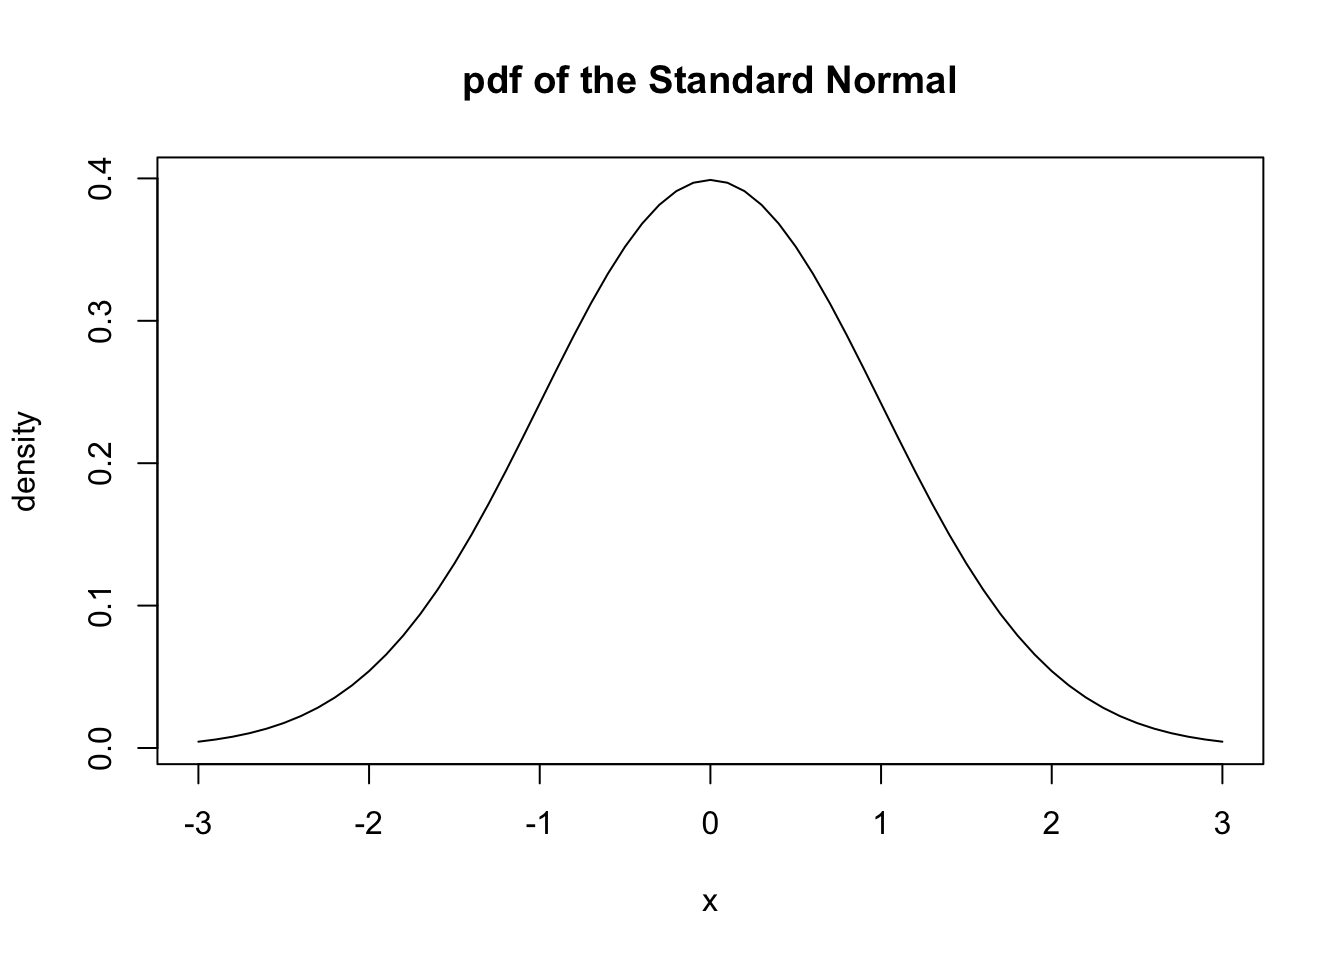
\includegraphics{index_files/figure-latex/unnamed-chunk-46-1.pdf}

Of course, you could create a data frame with these values and then use
ggplot if you want to:

\begin{Shaded}
\begin{Highlighting}[]
\NormalTok{std_norm =}\StringTok{ }\KeywordTok{data.frame}\NormalTok{(}\DataTypeTok{x=}\NormalTok{ x_vals,}\DataTypeTok{y=}\NormalTok{y_vals)}

\KeywordTok{ggplot}\NormalTok{(}\DataTypeTok{data =}\NormalTok{ std_norm) }\OperatorTok{+}
\StringTok{  }\KeywordTok{geom_line}\NormalTok{(}\DataTypeTok{mapping =} \KeywordTok{aes}\NormalTok{(}\DataTypeTok{x =}\NormalTok{ x,}\DataTypeTok{y=}\NormalTok{y))}
\end{Highlighting}
\end{Shaded}

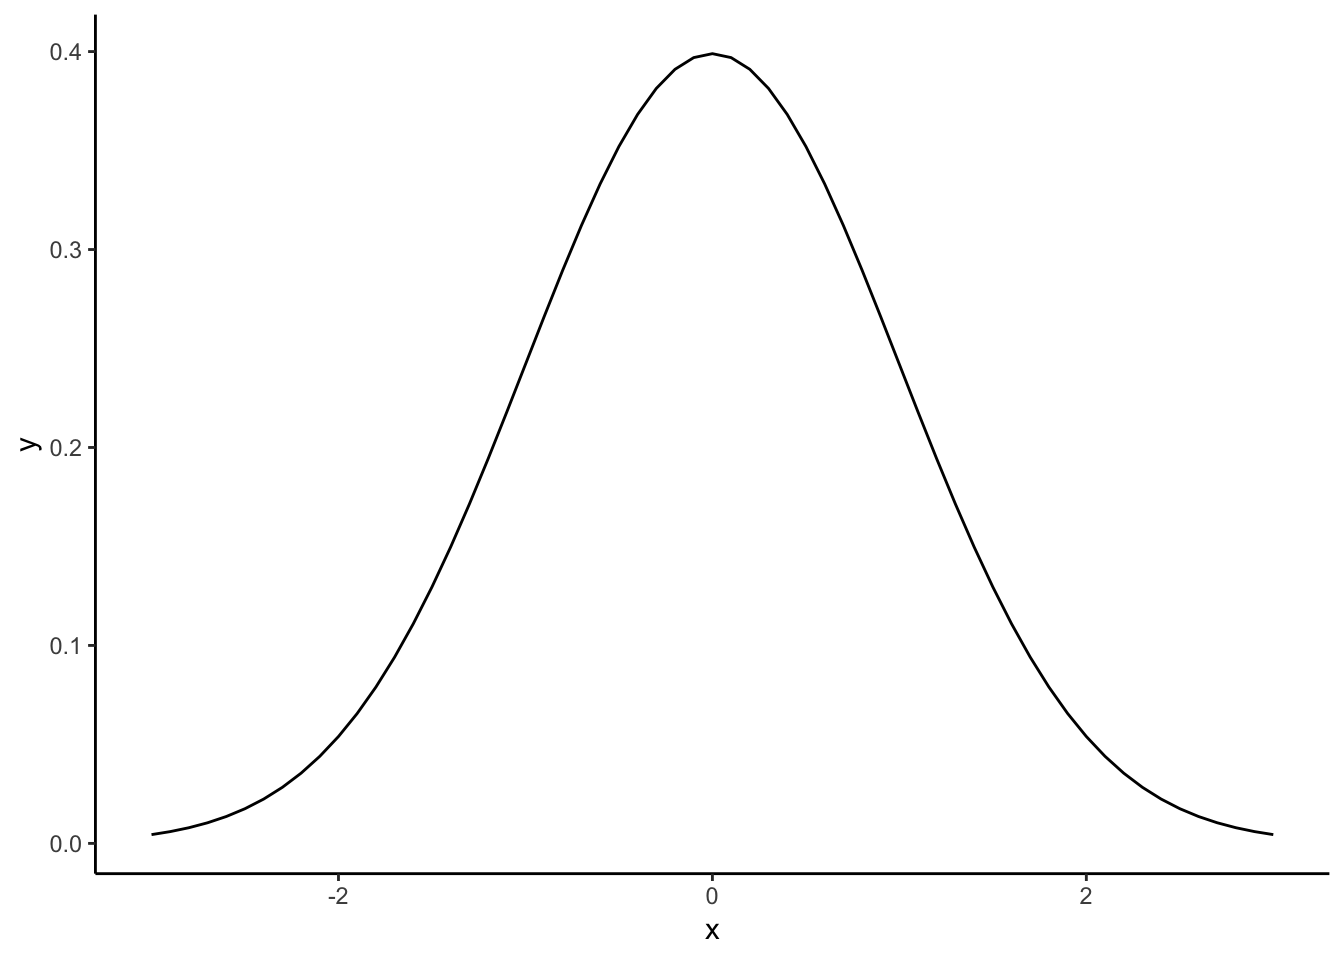
\includegraphics{index_files/figure-latex/unnamed-chunk-47-1.pdf}

The other three most relevant functions are: \emph{pnorm} (cumulative
distribution function), \emph{qnorm} (quantiles) and \emph{rnorm} (draw
random numbers). The ue of \emph{pnorm} is completely analogous to
\emph{dnorm}, so we skip it here and focus on themore interesting
\emph{qnorm} and \emph{rnorm}.

\hypertarget{quantiles}{%
\subsection{Quantiles}\label{quantiles}}

The function qnorm gives us the quantiles of the normal distirbution:

\begin{Shaded}
\begin{Highlighting}[]
\CommentTok{# Let's make a vector of : }
\CommentTok{# from 0 to 1 by increments of .05}
\NormalTok{quantiles <-}\StringTok{ }\KeywordTok{seq}\NormalTok{(}\DecValTok{0}\NormalTok{, }\DecValTok{1}\NormalTok{, }\DataTypeTok{by =} \FloatTok{.05}\NormalTok{)}
\NormalTok{quantiles}
\end{Highlighting}
\end{Shaded}

\begin{verbatim}
##  [1] 0.00 0.05 0.10 0.15 0.20 0.25 0.30 0.35 0.40 0.45 0.50 0.55 0.60 0.65
## [15] 0.70 0.75 0.80 0.85 0.90 0.95 1.00
\end{verbatim}

\begin{Shaded}
\begin{Highlighting}[]
\CommentTok{# Now we'll find the value for each of those quantiles}
\CommentTok{# Remeber that the q-quantile is the value Q such that}
\CommentTok{# P(X>Q) = q }
\CommentTok{# In other words, the quantile is the inverse of the CDF}

\NormalTok{qvalues <-}\StringTok{ }\KeywordTok{qnorm}\NormalTok{(quantiles)}
\NormalTok{qvalues}
\end{Highlighting}
\end{Shaded}

\begin{verbatim}
##  [1]       -Inf -1.6448536 -1.2815516 -1.0364334 -0.8416212 -0.6744898
##  [7] -0.5244005 -0.3853205 -0.2533471 -0.1256613  0.0000000  0.1256613
## [13]  0.2533471  0.3853205  0.5244005  0.6744898  0.8416212  1.0364334
## [19]  1.2815516  1.6448536        Inf
\end{verbatim}

We could now plot the PDF of a normal distirbution and illustrate a few
of the concepts:

\begin{Shaded}
\begin{Highlighting}[]
\KeywordTok{plot}\NormalTok{(x_vals,y_vals, }
     \DataTypeTok{type =} \StringTok{"l"}\NormalTok{, }\CommentTok{# Make it a line plot}
     \DataTypeTok{main =} \StringTok{"pdf of the Standard Normal"}\NormalTok{,}
     \DataTypeTok{xlab=} \StringTok{"x"}\NormalTok{,}\DataTypeTok{ylab=}\StringTok{"density"}\NormalTok{) }

\CommentTok{# the 50 % quantile is just the median:}
\KeywordTok{abline}\NormalTok{(}\DataTypeTok{v =} \KeywordTok{qnorm}\NormalTok{(}\FloatTok{0.5}\NormalTok{),}\DataTypeTok{col=}\StringTok{"black"}\NormalTok{,}\DataTypeTok{lwd=}\DecValTok{2}\NormalTok{,}\DataTypeTok{lty=}\DecValTok{1}\NormalTok{)}

\CommentTok{# the 2.5 %  and the 97.5% quantile indicated the area where 95% of the most }
\CommentTok{# common data lies:}
\KeywordTok{abline}\NormalTok{(}\DataTypeTok{v =} \KeywordTok{qnorm}\NormalTok{(}\KeywordTok{c}\NormalTok{(}\FloatTok{0.025}\NormalTok{,}\FloatTok{0.975}\NormalTok{)),}\DataTypeTok{col=}\StringTok{"darkred"}\NormalTok{,}\DataTypeTok{lwd=}\DecValTok{2}\NormalTok{,}\DataTypeTok{lty=}\DecValTok{2}\NormalTok{)}
\KeywordTok{text}\NormalTok{(}\OperatorTok{-}\FloatTok{2.5}\NormalTok{,}\FloatTok{0.3}\NormalTok{,}\StringTok{"qnorm(0.025)"}\NormalTok{,}\DataTypeTok{col=}\StringTok{"darkred"}\NormalTok{)}

\CommentTok{# In contrast, the function dnorm gives us the value of the PDF}
\CommentTok{# for a specfific x value, that is, the height of the function f(x) }
\CommentTok{# at the point x}

\KeywordTok{abline}\NormalTok{(}\DataTypeTok{h =} \KeywordTok{dnorm}\NormalTok{(}\OperatorTok{-}\DecValTok{1}\NormalTok{),}\DataTypeTok{col=}\StringTok{"blue"}\NormalTok{,}\DataTypeTok{lwd=}\DecValTok{2}\NormalTok{,}\DataTypeTok{lty=}\DecValTok{1}\NormalTok{)}
\KeywordTok{abline}\NormalTok{(}\DataTypeTok{v =} \DecValTok{-1}\NormalTok{,}\DataTypeTok{lty=}\DecValTok{2}\NormalTok{)}
\KeywordTok{text}\NormalTok{(}\OperatorTok{-}\FloatTok{1.4}\NormalTok{,}\FloatTok{0.25}\NormalTok{,}\StringTok{"dnorm(-1)"}\NormalTok{,}\DataTypeTok{col=}\StringTok{"blue"}\NormalTok{)}
\end{Highlighting}
\end{Shaded}

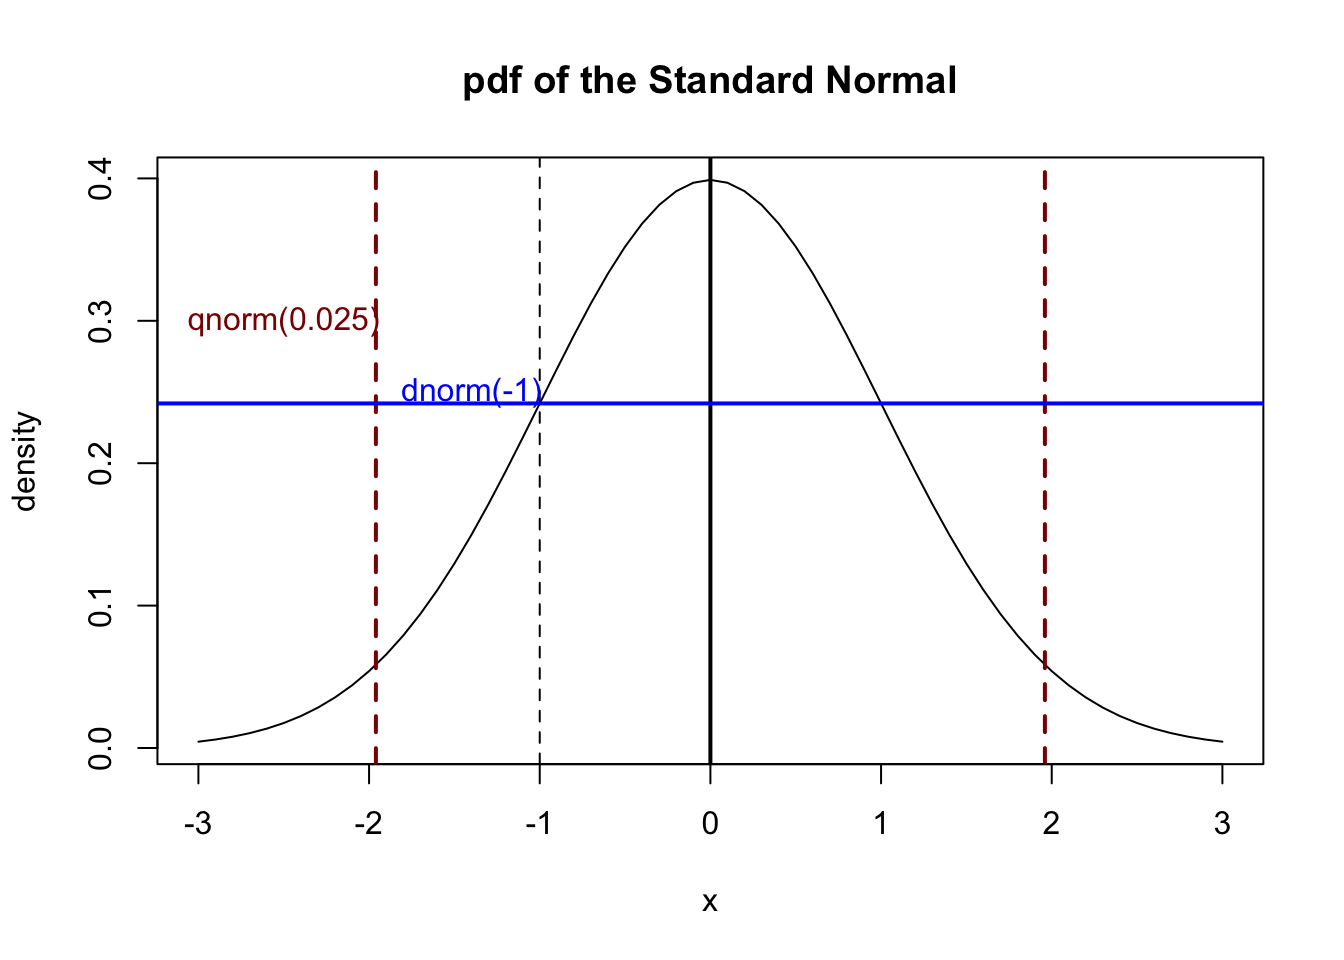
\includegraphics{index_files/figure-latex/unnamed-chunk-49-1.pdf}

\hypertarget{drawing-random-numbers}{%
\subsection{Drawing random numbers}\label{drawing-random-numbers}}

R also allows us to draw random numbers. This is very handy in many
situations. The parameters of rnorm are

\begin{itemize}
\item
  the number of observations
\item
  the mean of the distirbution
\item
  the standard deviation of the distribution
\end{itemize}

Here is an example, where we calculate a sample of 0, 100 and 1000
observations of the same distirbution.

\begin{Shaded}
\begin{Highlighting}[]
\CommentTok{# Let's generate three different vectors of random numbers }
\CommentTok{# from a normal  distribution}
\NormalTok{n10 <-}\StringTok{ }\KeywordTok{rnorm}\NormalTok{(}\DecValTok{10}\NormalTok{, }\DataTypeTok{mean =} \DecValTok{70}\NormalTok{, }\DataTypeTok{sd =} \DecValTok{5}\NormalTok{)}
\NormalTok{n100 <-}\StringTok{ }\KeywordTok{rnorm}\NormalTok{(}\DecValTok{100}\NormalTok{, }\DataTypeTok{mean =} \DecValTok{70}\NormalTok{, }\DataTypeTok{sd =} \DecValTok{5}\NormalTok{)}
\NormalTok{n10000 <-}\StringTok{  }\KeywordTok{rnorm}\NormalTok{(}\DecValTok{10000}\NormalTok{, }\DataTypeTok{mean =} \DecValTok{70}\NormalTok{, }\DataTypeTok{sd =} \DecValTok{5}\NormalTok{)}

\CommentTok{# Let's just look at one of the vectors}
\NormalTok{n10}
\end{Highlighting}
\end{Shaded}

\begin{verbatim}
##  [1] 70.99053 62.81864 75.27632 67.91037 72.28005 73.18971 68.06684
##  [8] 66.27608 72.51235 69.68982
\end{verbatim}

\begin{Shaded}
\begin{Highlighting}[]
\CommentTok{# The breaks argument specifies how many bars are in the histogram}
\KeywordTok{hist}\NormalTok{(n10, }\DataTypeTok{breaks =} \DecValTok{5}\NormalTok{)}
\end{Highlighting}
\end{Shaded}

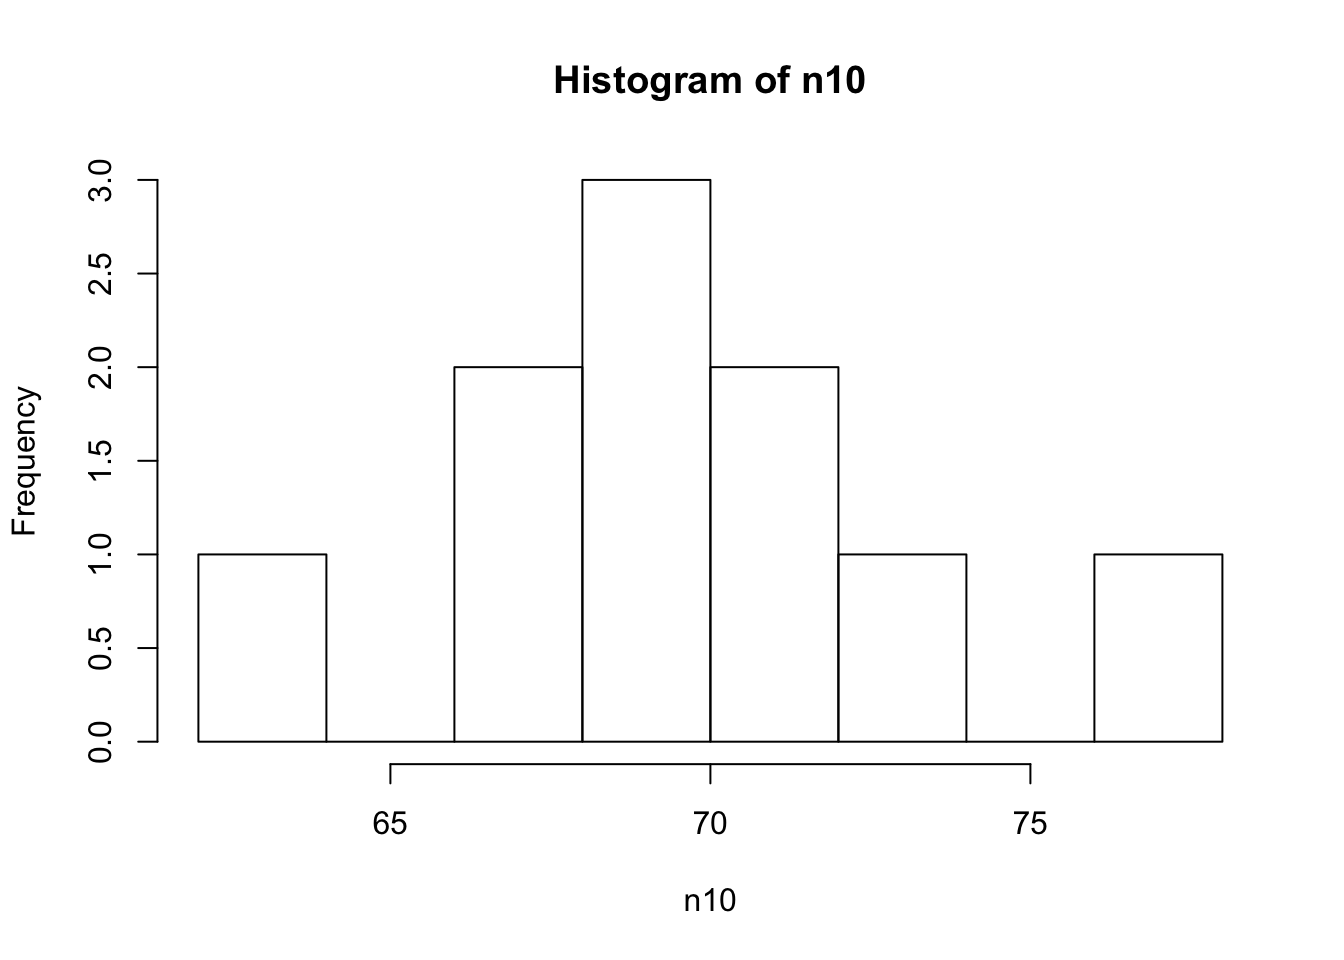
\includegraphics{index_files/figure-latex/unnamed-chunk-50-1.pdf}

\begin{Shaded}
\begin{Highlighting}[]
\KeywordTok{hist}\NormalTok{(n100, }\DataTypeTok{breaks =} \DecValTok{20}\NormalTok{)}
\end{Highlighting}
\end{Shaded}

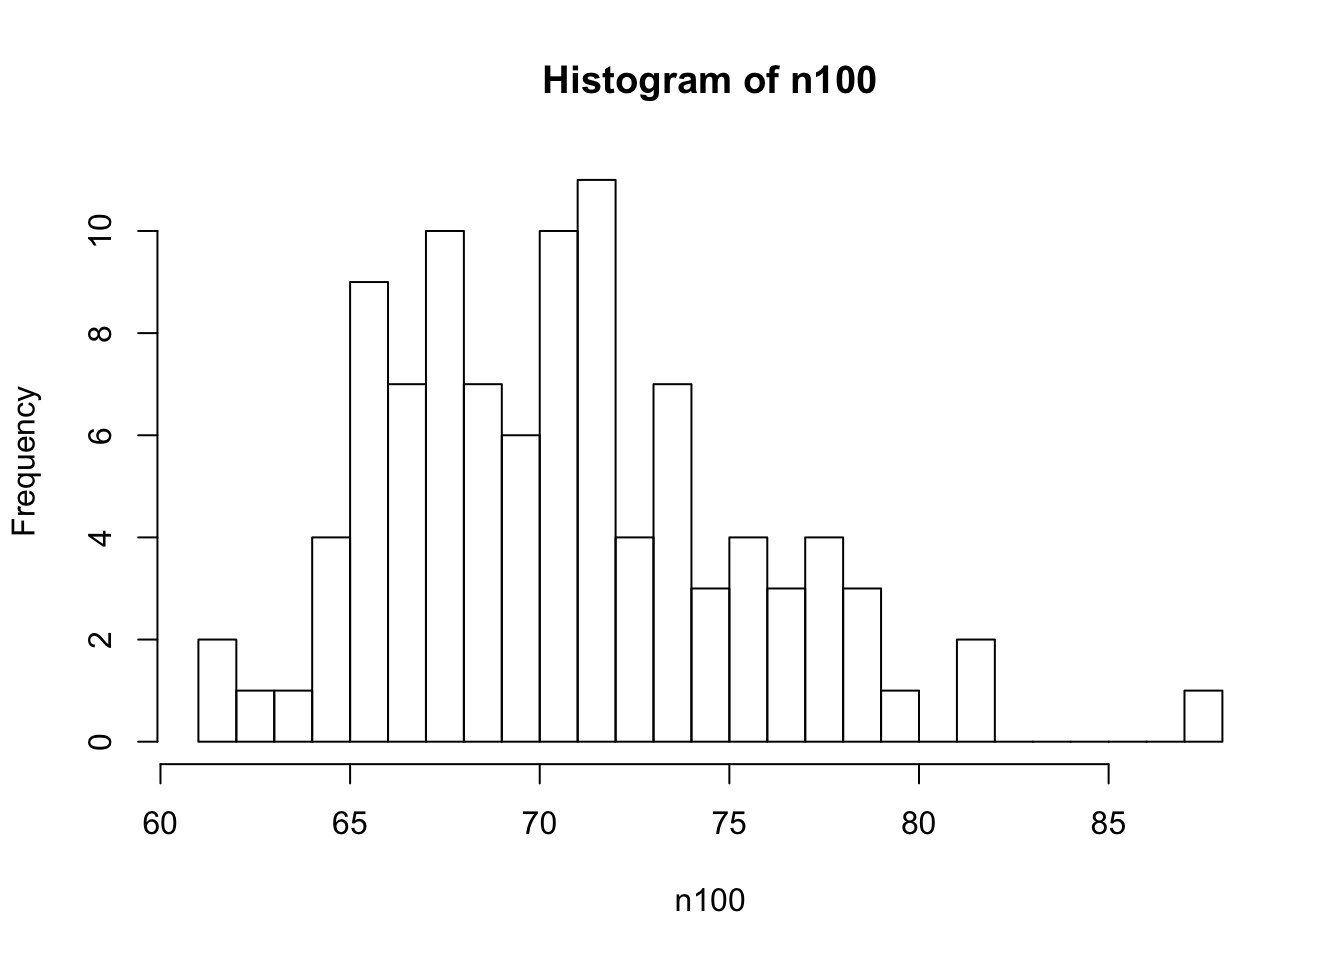
\includegraphics{index_files/figure-latex/unnamed-chunk-50-2.pdf}

\begin{Shaded}
\begin{Highlighting}[]
\KeywordTok{hist}\NormalTok{(n10000, }\DataTypeTok{breaks =} \DecValTok{100}\NormalTok{)}
\end{Highlighting}
\end{Shaded}

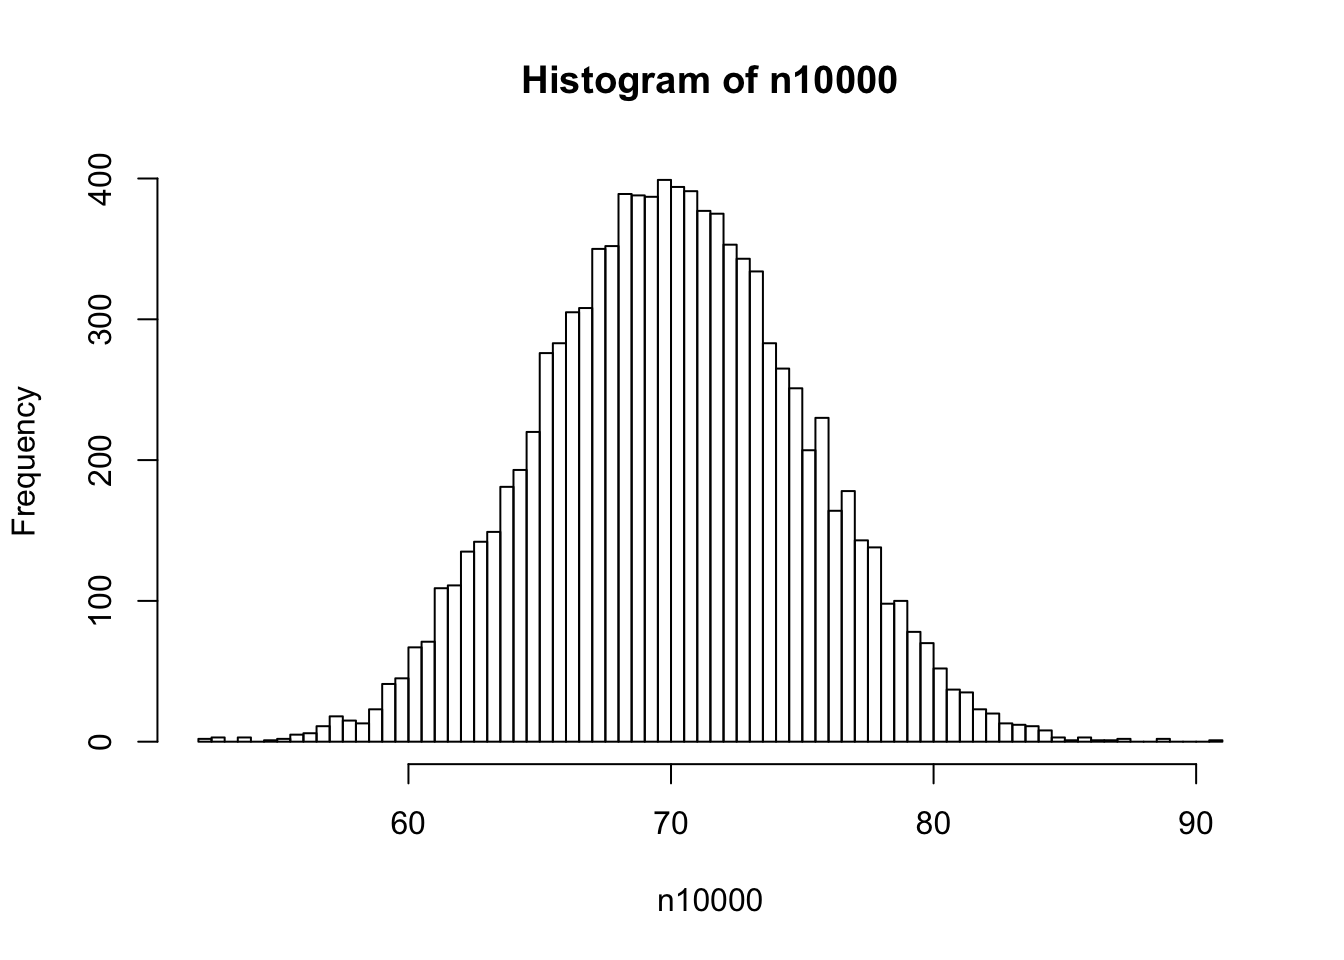
\includegraphics{index_files/figure-latex/unnamed-chunk-50-3.pdf}

\emph{Note:} If we set a \emph{seed} for our random number generator
(the algorithm that is used to calcualte a radnom number), we can make
our analysis replicable:

\begin{Shaded}
\begin{Highlighting}[]
\KeywordTok{set.seed}\NormalTok{(}\DecValTok{100}\NormalTok{)}
\KeywordTok{rnorm}\NormalTok{(}\DecValTok{1}\NormalTok{,}\DecValTok{0}\NormalTok{,}\DecValTok{1}\NormalTok{)}
\end{Highlighting}
\end{Shaded}

\begin{verbatim}
## [1] -0.5021924
\end{verbatim}

\begin{Shaded}
\begin{Highlighting}[]
\KeywordTok{rnorm}\NormalTok{(}\DecValTok{1}\NormalTok{,}\DecValTok{0}\NormalTok{,}\DecValTok{1}\NormalTok{)}
\end{Highlighting}
\end{Shaded}

\begin{verbatim}
## [1] 0.1315312
\end{verbatim}

\begin{Shaded}
\begin{Highlighting}[]
\KeywordTok{set.seed}\NormalTok{(}\DecValTok{100}\NormalTok{)}
\KeywordTok{rnorm}\NormalTok{(}\DecValTok{1}\NormalTok{,}\DecValTok{0}\NormalTok{,}\DecValTok{1}\NormalTok{)}
\end{Highlighting}
\end{Shaded}

\begin{verbatim}
## [1] -0.5021924
\end{verbatim}

\begin{Shaded}
\begin{Highlighting}[]
\KeywordTok{rnorm}\NormalTok{(}\DecValTok{1}\NormalTok{,}\DecValTok{0}\NormalTok{,}\DecValTok{1}\NormalTok{)}
\end{Highlighting}
\end{Shaded}

\begin{verbatim}
## [1] 0.1315312
\end{verbatim}

\hypertarget{plotting-confidence-intervalls}{%
\subsection{Plotting Confidence
intervalls}\label{plotting-confidence-intervalls}}

We first generate a data frame with a summary of our data (this can be
done in many ways, this is a concise one):

\begin{Shaded}
\begin{Highlighting}[]
\NormalTok{CIs <-}\StringTok{ }\KeywordTok{summarySE}\NormalTok{(stickleback, }\DataTypeTok{measurevar=}\StringTok{"plates"}\NormalTok{, }\DataTypeTok{groupvars=}\KeywordTok{c}\NormalTok{(}\StringTok{"genotype"}\NormalTok{))}

\NormalTok{CIs}
\end{Highlighting}
\end{Shaded}

\begin{verbatim}
##   genotype   N   plates        sd        se        ci
## 1       MM  82 62.78049  3.410313 0.3766060 0.7493279
## 2       Mm 174 50.37931 15.146866 1.1482809 2.2664440
## 3       mm  88 11.67045  3.567805 0.3803293 0.7559456
\end{verbatim}

and then we use the data frame with our summary to add error bars to our
plot:

\begin{Shaded}
\begin{Highlighting}[]
\KeywordTok{ggplot}\NormalTok{(}\DataTypeTok{data =}\NormalTok{ CIs) }\OperatorTok{+}
\StringTok{  }\KeywordTok{geom_point}\NormalTok{(}\DataTypeTok{mapping =} \KeywordTok{aes}\NormalTok{(}\DataTypeTok{x =}\NormalTok{ genotype,}\DataTypeTok{y=}\NormalTok{plates)) }\OperatorTok{+}
\StringTok{  }\KeywordTok{geom_errorbar}\NormalTok{(}\DataTypeTok{mapping =} \KeywordTok{aes}\NormalTok{(}\DataTypeTok{x =}\NormalTok{ genotype,}\DataTypeTok{y=}\NormalTok{plates,}\DataTypeTok{ymin=}\NormalTok{plates}\OperatorTok{-}\NormalTok{ci, }\DataTypeTok{ymax=}\NormalTok{plates}\OperatorTok{+}\NormalTok{ci), }\DataTypeTok{width=}\NormalTok{.}\DecValTok{1}\NormalTok{) }
\end{Highlighting}
\end{Shaded}

\begin{verbatim}
## Warning: Ignoring unknown aesthetics: y
\end{verbatim}

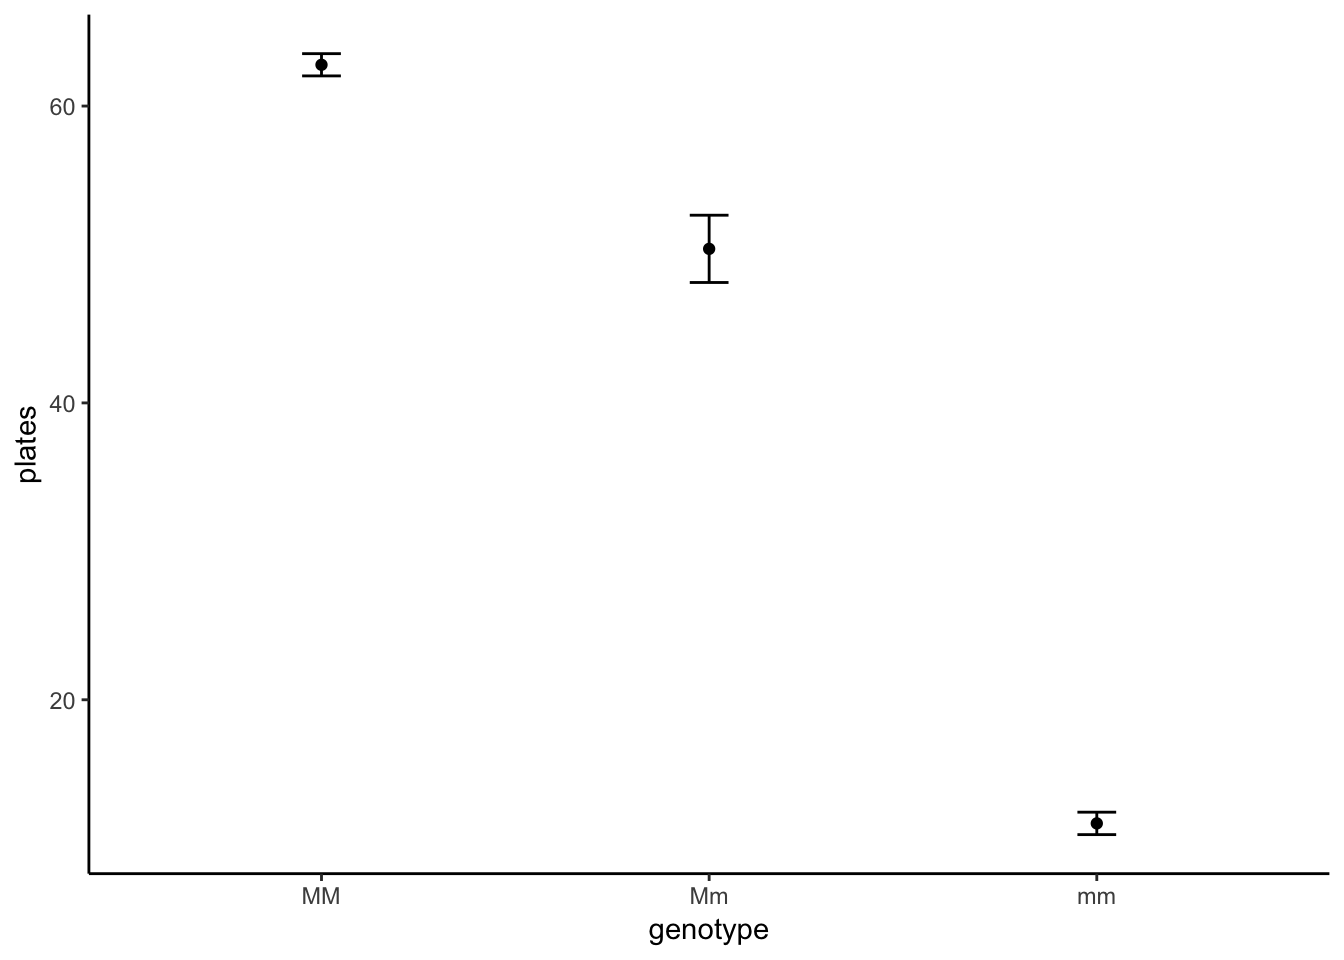
\includegraphics{index_files/figure-latex/unnamed-chunk-53-1.pdf}

\emph{Note:} One can shorten things by specifying the aesthetics in the
ggplot command - this simply means that all geom\_functions use the same
x and y variables (which is very often the case, but not always!):

\begin{Shaded}
\begin{Highlighting}[]
\KeywordTok{ggplot}\NormalTok{(}\DataTypeTok{data =}\NormalTok{ CIs, }\KeywordTok{aes}\NormalTok{(}\DataTypeTok{x =}\NormalTok{ genotype,}\DataTypeTok{y=}\NormalTok{plates)) }\OperatorTok{+}
\StringTok{  }\KeywordTok{geom_point}\NormalTok{() }\OperatorTok{+}
\StringTok{  }\KeywordTok{geom_errorbar}\NormalTok{(}\DataTypeTok{mapping =} \KeywordTok{aes}\NormalTok{(}\DataTypeTok{ymin=}\NormalTok{plates}\OperatorTok{-}\NormalTok{ci, }\DataTypeTok{ymax=}\NormalTok{plates}\OperatorTok{+}\NormalTok{ci), }\DataTypeTok{width=}\NormalTok{.}\DecValTok{1}\NormalTok{) }
\end{Highlighting}
\end{Shaded}

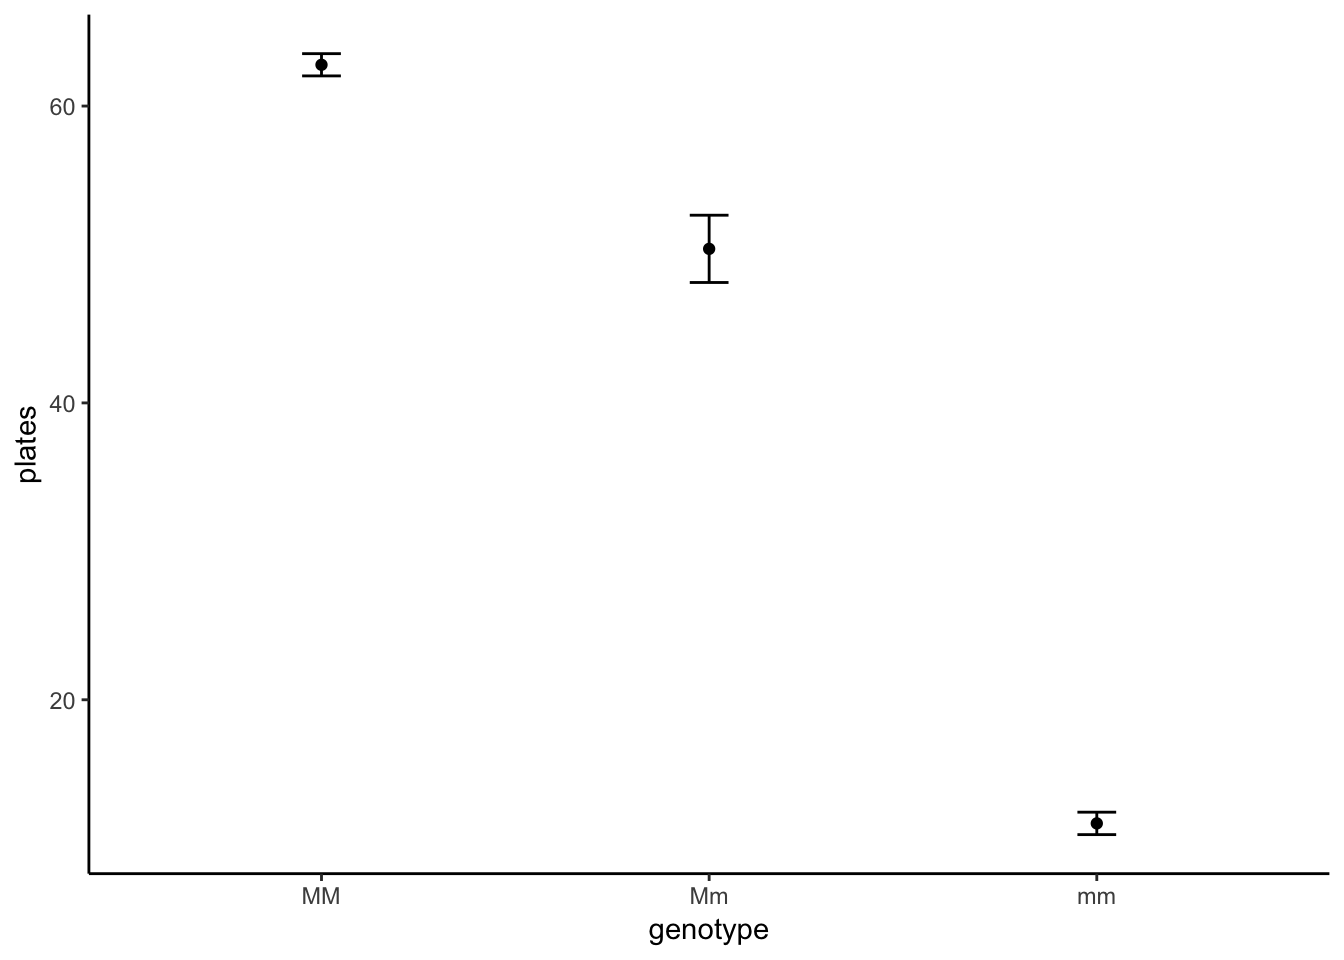
\includegraphics{index_files/figure-latex/unnamed-chunk-54-1.pdf}

\emph{Note:} The function \emph{t.test()} can also be used to calcualte
confidence intervalls assuming a normal distribution.

\begin{Shaded}
\begin{Highlighting}[]
\NormalTok{genotpyes =}\StringTok{ }\KeywordTok{c}\NormalTok{(}\StringTok{"MM"}\NormalTok{,}\StringTok{"Mm"}\NormalTok{,}\StringTok{"mm"}\NormalTok{) }
\NormalTok{CI.upper =}\StringTok{ }\KeywordTok{vector}\NormalTok{(}\StringTok{"numeric"}\NormalTok{,}\DecValTok{3}\NormalTok{)}
\NormalTok{CI.lower =}\StringTok{ }\KeywordTok{vector}\NormalTok{(}\StringTok{"numeric"}\NormalTok{,}\DecValTok{3}\NormalTok{)}
\NormalTok{means =}\StringTok{ }\KeywordTok{vector}\NormalTok{(}\StringTok{"numeric"}\NormalTok{,}\DecValTok{3}\NormalTok{)}

\NormalTok{i =}\StringTok{ }\DecValTok{1}

\ControlFlowTok{for}\NormalTok{(g }\ControlFlowTok{in}\NormalTok{ genotypes)}
\NormalTok{\{}
  
\NormalTok{  results =}\StringTok{ }\KeywordTok{t.test}\NormalTok{(stickleback}\OperatorTok{$}\NormalTok{plates[stickleback}\OperatorTok{$}\NormalTok{genotype }\OperatorTok{==}\StringTok{ }\NormalTok{g])}
  
\NormalTok{  CI.lower[i] =}\StringTok{ }\NormalTok{results}\OperatorTok{$}\NormalTok{conf.int[}\DecValTok{1}\NormalTok{]}
\NormalTok{  CI.upper[i]=}\StringTok{ }\NormalTok{results}\OperatorTok{$}\NormalTok{conf.int[}\DecValTok{2}\NormalTok{]}
\NormalTok{  means[i] =}\StringTok{ }\NormalTok{results}\OperatorTok{$}\NormalTok{estimate}
\NormalTok{  i =}\StringTok{ }\NormalTok{i }\OperatorTok{+}\StringTok{ }\DecValTok{1}
\NormalTok{\}}

\NormalTok{CI.data =}\StringTok{ }\KeywordTok{data.frame}\NormalTok{(}\DataTypeTok{genotype =}\NormalTok{ genotpyes,}\DataTypeTok{mean =}\NormalTok{ means,}\DataTypeTok{CI.lower =}\NormalTok{ CI.lower,}\DataTypeTok{CI.upper =}\NormalTok{ CI.upper)}

\KeywordTok{ggplot}\NormalTok{(}\DataTypeTok{data =}\NormalTok{ CI.data, }\KeywordTok{aes}\NormalTok{(}\DataTypeTok{x =}\NormalTok{ genotype,}\DataTypeTok{y=}\NormalTok{means)) }\OperatorTok{+}
\StringTok{  }\KeywordTok{geom_point}\NormalTok{() }\OperatorTok{+}
\StringTok{  }\KeywordTok{geom_errorbar}\NormalTok{(}\DataTypeTok{mapping =} \KeywordTok{aes}\NormalTok{(}\DataTypeTok{ymin=}\NormalTok{CI.lower, }\DataTypeTok{ymax=}\NormalTok{CI.upper), }\DataTypeTok{width=}\NormalTok{.}\DecValTok{1}\NormalTok{) }
\end{Highlighting}
\end{Shaded}

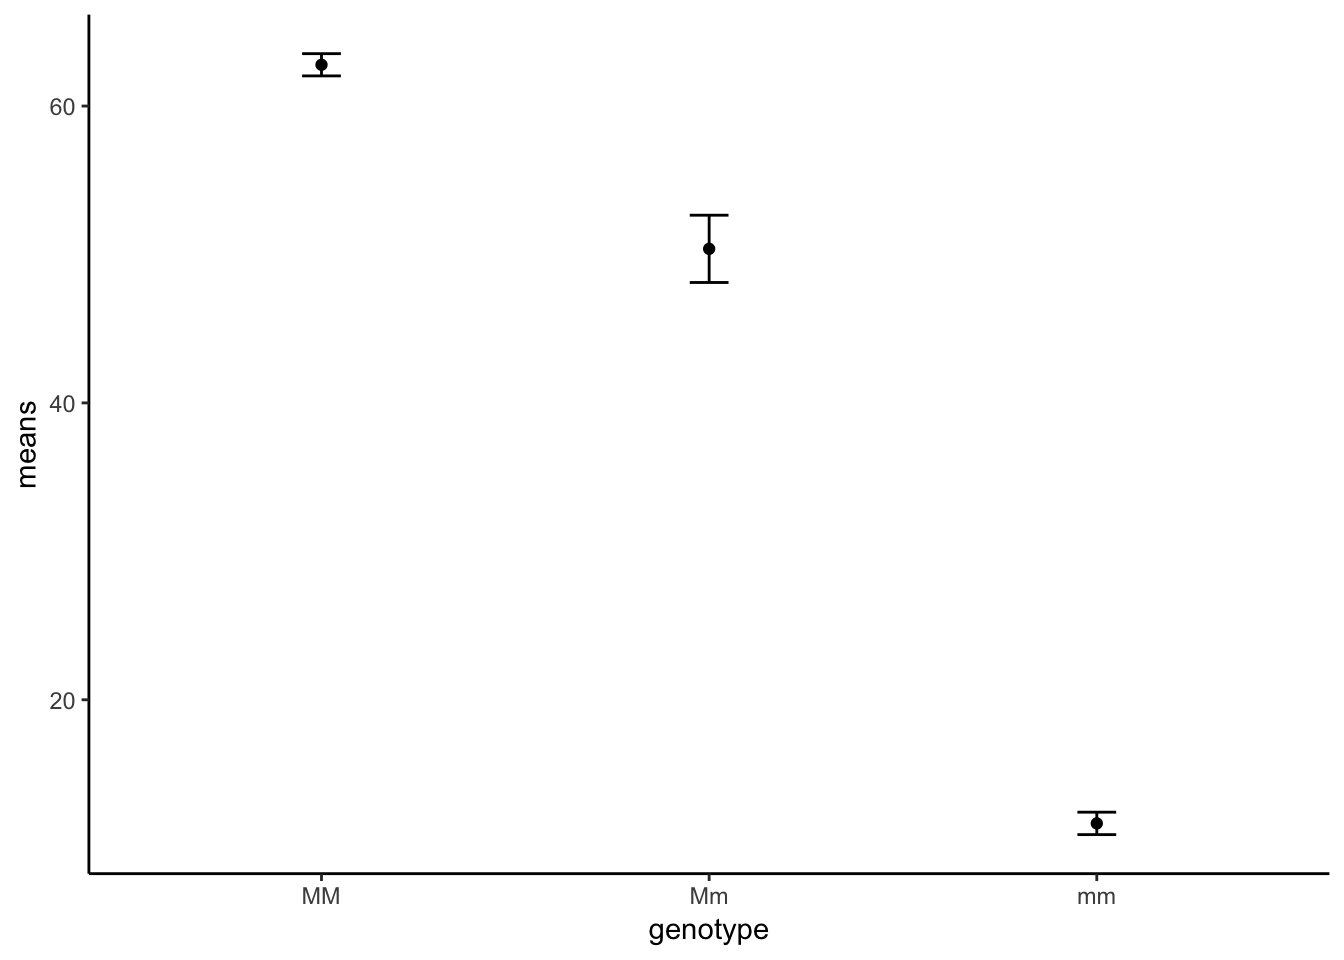
\includegraphics{index_files/figure-latex/unnamed-chunk-55-1.pdf}

\hypertarget{putting-everything-together-a-simple-simulation}{%
\subsection{Putting everything together: A simple
simulation}\label{putting-everything-together-a-simple-simulation}}

Copy and paste this R code into a script. Before you run it, try to
figure out what it does.

\begin{Shaded}
\begin{Highlighting}[]
\NormalTok{reps =}\StringTok{ }\DecValTok{1000}
\NormalTok{sample_size =}\StringTok{ }\DecValTok{10}
\NormalTok{mu =}\StringTok{ }\DecValTok{10}
\NormalTok{sigma =}\StringTok{ }\DecValTok{5}
\NormalTok{means =}\StringTok{ }\KeywordTok{vector}\NormalTok{(}\StringTok{"numeric"}\NormalTok{,reps)}

\ControlFlowTok{for}\NormalTok{ (i }\ControlFlowTok{in} \DecValTok{1}\OperatorTok{:}\NormalTok{reps)}
\NormalTok{\{}
\NormalTok{  sample =}\StringTok{ }\KeywordTok{rnorm}\NormalTok{(sample_size,mu,sigma)}
\NormalTok{  means[i] =}\StringTok{ }\KeywordTok{mean}\NormalTok{(sample)}
\NormalTok{\}}

\KeywordTok{hist}\NormalTok{(means,}\DataTypeTok{freq=}\NormalTok{F,}\DataTypeTok{main=}\StringTok{"A distribution"}\NormalTok{)}

\NormalTok{x =}\StringTok{ }\KeywordTok{seq}\NormalTok{(mu}\DecValTok{-2}\OperatorTok{*}\NormalTok{sigma,mu}\OperatorTok{+}\DecValTok{2}\OperatorTok{*}\NormalTok{sigma,}\DataTypeTok{by=}\FloatTok{0.01}\NormalTok{)}

\NormalTok{SE =}\StringTok{ }\NormalTok{sigma}\OperatorTok{/}\KeywordTok{sqrt}\NormalTok{(sample_size)}

\NormalTok{y =}\StringTok{ }\KeywordTok{dnorm}\NormalTok{(x,mu,SE)}

\KeywordTok{lines}\NormalTok{(x,y)}
\end{Highlighting}
\end{Shaded}

\hypertarget{hypothesis-tests}{%
\section{Hypothesis Tests}\label{hypothesis-tests}}

In this chpater we will learn how to do hypotehsis tests in R. This is
very simple, as you will see - often a single line of code is sufficient
for conducting a test.

\hypertarget{binomial-test}{%
\subsection{Binomial-test}\label{binomial-test}}

We use the binomial test to test whether spermatogenesis genes in the
mouse genome occur with unusual frequency on the X chromosome. First, we
load the dat set and inspect it:

\begin{Shaded}
\begin{Highlighting}[]
\NormalTok{mouseGenes <-}\StringTok{ }\KeywordTok{read_csv}\NormalTok{(}\StringTok{"~/Dropbox/Teaching/StatisticsForBiology/chap07e2SexAndX.csv"}\NormalTok{)}

\KeywordTok{head}\NormalTok{(mouseGenes)}
\end{Highlighting}
\end{Shaded}

\begin{verbatim}
## # A tibble: 6 x 2
##   chromosome onX  
##   <chr>      <chr>
## 1 4          no   
## 2 4          no   
## 3 6          no   
## 4 6          no   
## 5 6          no   
## 6 7          no
\end{verbatim}

\begin{Shaded}
\begin{Highlighting}[]
\CommentTok{# Tabulate the number of spermatogenesis genes on the }
\CommentTok{# X-chromosome and the number not on the X-chromosome.}

\KeywordTok{table}\NormalTok{(mouseGenes}\OperatorTok{$}\NormalTok{onX)}
\end{Highlighting}
\end{Shaded}

\begin{verbatim}
## 
##  no yes 
##  15  10
\end{verbatim}

\begin{Shaded}
\begin{Highlighting}[]
\CommentTok{# Calculate the binomial probabilities of all possible outcomes}
\CommentTok{# under the null hypothesis. Under the binomial}
\CommentTok{# distribution with n = 25 and p = 0.061, the number of successes}
\CommentTok{# can be any integer between 0 and 25.}

\NormalTok{xsuccesses <-}\StringTok{ }\DecValTok{0}\OperatorTok{:}\DecValTok{25}
\NormalTok{probx <-}\StringTok{ }\KeywordTok{dbinom}\NormalTok{(xsuccesses, }\DataTypeTok{size =} \DecValTok{25}\NormalTok{, }\DataTypeTok{prob =} \FloatTok{0.061}\NormalTok{)}
\KeywordTok{data.frame}\NormalTok{(xsuccesses, probx)}
\end{Highlighting}
\end{Shaded}

\begin{verbatim}
##    xsuccesses        probx
## 1           0 2.073193e-01
## 2           1 3.367007e-01
## 3           2 2.624760e-01
## 4           3 1.307255e-01
## 5           4 4.670757e-02
## 6           5 1.274386e-02
## 7           6 2.759585e-03
## 8           7 4.865905e-04
## 9           8 7.112305e-05
## 10          9 8.727323e-06
## 11         10 9.071211e-07
## 12         11 8.035781e-08
## 13         12 6.090306e-09
## 14         13 3.956429e-10
## 15         14 2.203032e-11
## 16         15 1.049510e-12
## 17         16 4.261188e-14
## 18         17 1.465509e-15
## 19         18 4.231266e-17
## 20         19 1.012696e-18
## 21         20 1.973624e-20
## 22         21 3.052667e-22
## 23         22 3.605629e-24
## 24         23 3.055193e-26
## 25         24 1.653947e-28
## 26         25 4.297797e-31
\end{verbatim}

\begin{Shaded}
\begin{Highlighting}[]
\KeywordTok{barplot}\NormalTok{(probx,}\DataTypeTok{names.arg=}\NormalTok{xsuccesses,}\DataTypeTok{xlab=}\StringTok{"# successes"}\NormalTok{,}\DataTypeTok{ylab=}\StringTok{"probability"}\NormalTok{)}
\end{Highlighting}
\end{Shaded}

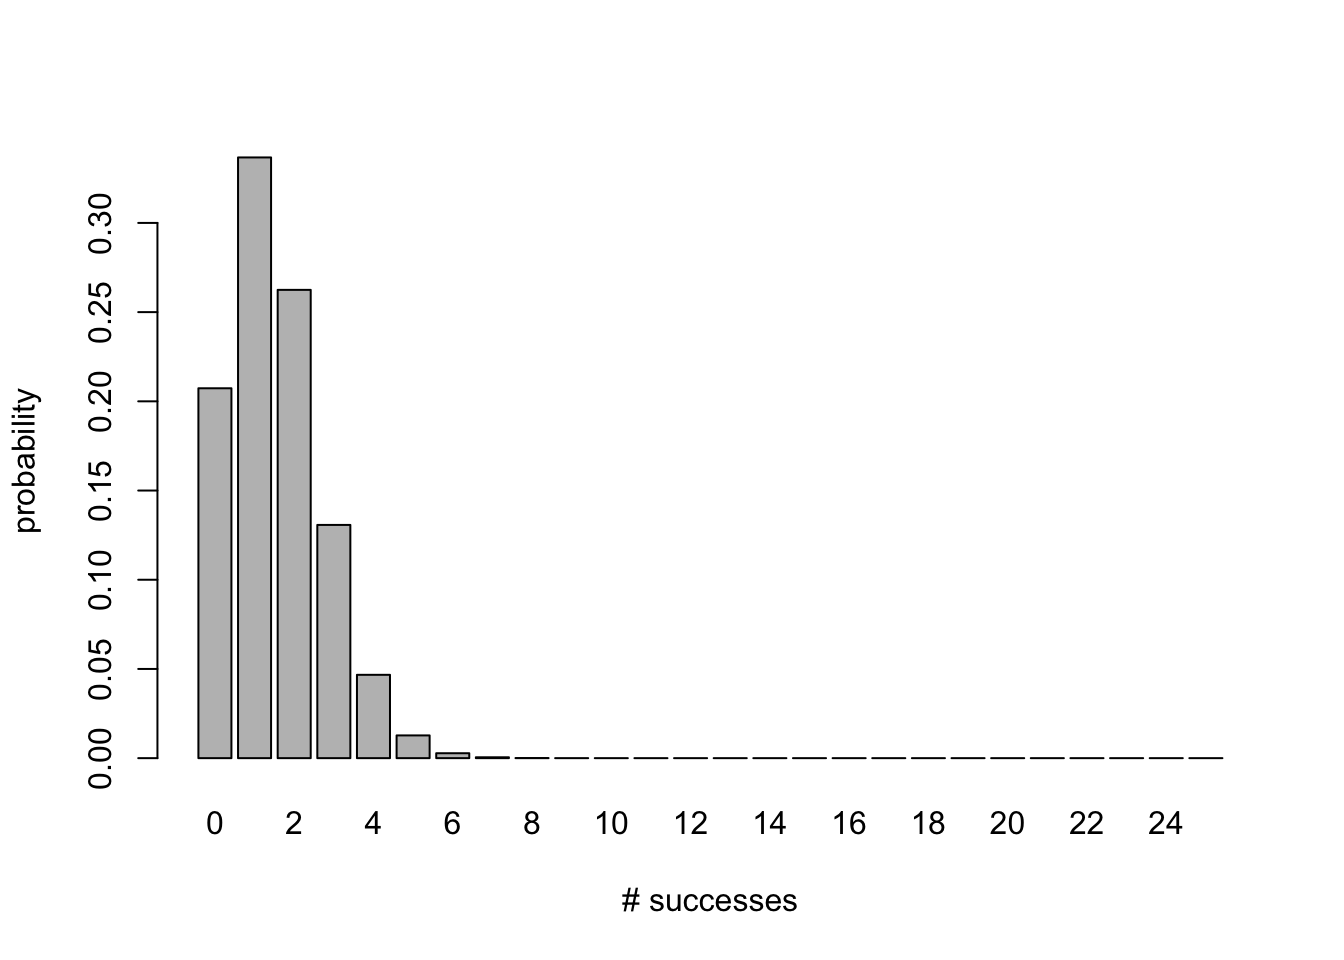
\includegraphics{index_files/figure-latex/unnamed-chunk-57-1.pdf}

\begin{Shaded}
\begin{Highlighting}[]
\CommentTok{# Use these probabilities to calculate the P-value corresponding to}
\CommentTok{# an observed 10 spermatogenesis genes on the X chromosome. }
\CommentTok{# Remember to multiply the probability of 10 or more successes }
\CommentTok{# by 2 for the two-tailed test result.}

\DecValTok{2} \OperatorTok{*}\StringTok{ }\KeywordTok{sum}\NormalTok{(probx[xsuccesses }\OperatorTok{>=}\StringTok{ }\DecValTok{10}\NormalTok{])}
\end{Highlighting}
\end{Shaded}

\begin{verbatim}
## [1] 1.987976e-06
\end{verbatim}

\begin{Shaded}
\begin{Highlighting}[]
\CommentTok{# For a faster result, try R's built-in binomial test. }
\CommentTok{# The resulting P-value is slightly different from our calculation. # The output of binom.test includes a confidence interval for the }
\CommentTok{# proportion using the Clopper-Pearson method, which is more }
\CommentTok{# conservative than the Agresti-Coull method.}

\KeywordTok{binom.test}\NormalTok{(}\DecValTok{10}\NormalTok{, }\DataTypeTok{n =} \DecValTok{25}\NormalTok{, }\DataTypeTok{p =} \FloatTok{0.061}\NormalTok{)}
\end{Highlighting}
\end{Shaded}

\begin{verbatim}
## 
##  Exact binomial test
## 
## data:  10 and 25
## number of successes = 10, number of trials = 25, p-value =
## 9.94e-07
## alternative hypothesis: true probability of success is not equal to 0.061
## 95 percent confidence interval:
##  0.2112548 0.6133465
## sample estimates:
## probability of success 
##                    0.4
\end{verbatim}

\begin{Shaded}
\begin{Highlighting}[]
\CommentTok{# Agresti-Coull 95% confidence interval for the proportion }
\CommentTok{# using the binom package.}

\KeywordTok{library}\NormalTok{(binom)}
\KeywordTok{binom.confint}\NormalTok{(}\DecValTok{30}\NormalTok{, }\DataTypeTok{n =} \DecValTok{87}\NormalTok{, }\DataTypeTok{method =} \StringTok{"ac"}\NormalTok{)}
\end{Highlighting}
\end{Shaded}

\begin{verbatim}
##          method  x  n      mean     lower     upper
## 1 agresti-coull 30 87 0.3448276 0.2532164 0.4495625
\end{verbatim}

\hypertarget{chi2-test}{%
\subsection{\texorpdfstring{\(\chi^2\)
test}{\textbackslash{}chi\^{}2 test}}\label{chi2-test}}

We perform a goodness-of-fit test. We use a Poisson probability model
and fit it to frequency data on the number of marine invertebrate
extinctions per time block in the fossil record. We first read and
inspect the data. Each row is a time block, with the observed number of
extinctions listed.

The first step is to create a frequency table for the number of time
blocks in each number-of-extinctions category. The command table does
what's needed, but note that some extinction categories are not
represented (e.g., 0, 12 and 13 extinctions).

\begin{Shaded}
\begin{Highlighting}[]
\NormalTok{extinctTable <-}\StringTok{ }\KeywordTok{table}\NormalTok{(extinctData}\OperatorTok{$}\NormalTok{numberOfExtinctions)}
\KeywordTok{data.frame}\NormalTok{(}\DataTypeTok{Frequency =} \KeywordTok{addmargins}\NormalTok{(extinctTable))}
\end{Highlighting}
\end{Shaded}

\begin{verbatim}
##    Frequency.Var1 Frequency.Freq
## 1               1             13
## 2               2             15
## 3               3             16
## 4               4              7
## 5               5             10
## 6               6              4
## 7               7              2
## 8               8              1
## 9               9              2
## 10             10              1
## 11             11              1
## 12             14              1
## 13             16              2
## 14             20              1
## 15            Sum             76
\end{verbatim}

To remedy the problem of missing categories, we transform the original
variable into a factor (that is, a categorical variable) with all counts
between 0 and 20 as levels (note that 20 is not the maximum possible
number of extinctions, but it is a convenient cutoff for this table).

\begin{Shaded}
\begin{Highlighting}[]
\NormalTok{extinctData =}\StringTok{ }\KeywordTok{mutate}\NormalTok{(extinctData,}\DataTypeTok{nExtinctFactor =} \KeywordTok{factor}\NormalTok{(numberOfExtinctions, }\DataTypeTok{levels =} \KeywordTok{c}\NormalTok{(}\DecValTok{0}\OperatorTok{:}\DecValTok{20}\NormalTok{)))}
                     
\NormalTok{extinctTable2 <-}\StringTok{ }\KeywordTok{table}\NormalTok{(extinctData}\OperatorTok{$}\NormalTok{nExtinctFactor)}
\end{Highlighting}
\end{Shaded}

Estimate the mean number of extinctions per time block from the data.
The estimate is needed for the goodness-of-fit test.

\begin{Shaded}
\begin{Highlighting}[]
\NormalTok{meanExtinctions <-}\StringTok{ }\KeywordTok{mean}\NormalTok{(extinctData}\OperatorTok{$}\NormalTok{numberOfExtinctions)}
\NormalTok{meanExtinctions}
\end{Highlighting}
\end{Shaded}

\begin{verbatim}
## [1] 4.210526
\end{verbatim}

Calculate expected frequencies under the Poisson distribution using the
estimated mean. (For now, continue to use 20 extinctions as the cutoff,
but don't forget that the Poisson distribution includes the
number-of-extinctions categories 21, 22, 23, and so on.)

\begin{Shaded}
\begin{Highlighting}[]
\NormalTok{expectedProportion <-}\StringTok{ }\KeywordTok{dpois}\NormalTok{(}\DecValTok{0}\OperatorTok{:}\DecValTok{20}\NormalTok{, }\DataTypeTok{lambda =}\NormalTok{ meanExtinctions)}
\NormalTok{expectedFrequency <-}\StringTok{ }\NormalTok{expectedProportion }\OperatorTok{*}\StringTok{ }\DecValTok{76}
\end{Highlighting}
\end{Shaded}

Show the frequency distribution in a histogram.

\begin{Shaded}
\begin{Highlighting}[]
\KeywordTok{ggplot}\NormalTok{(extinctData) }\OperatorTok{+}
\StringTok{  }\KeywordTok{geom_histogram}\NormalTok{(}\DataTypeTok{mapping=} \KeywordTok{aes}\NormalTok{(}\DataTypeTok{x =}\NormalTok{numberOfExtinctions),}\DataTypeTok{fill =} \StringTok{"firebrick"}\NormalTok{,}\DataTypeTok{color=}\StringTok{"black"}\NormalTok{,}\DataTypeTok{bins=}\DecValTok{21}\NormalTok{)}\OperatorTok{+}\StringTok{    }
\StringTok{  }\KeywordTok{labs}\NormalTok{ (}\DataTypeTok{x=}\StringTok{"Number of extinctions"}\NormalTok{)}
\end{Highlighting}
\end{Shaded}

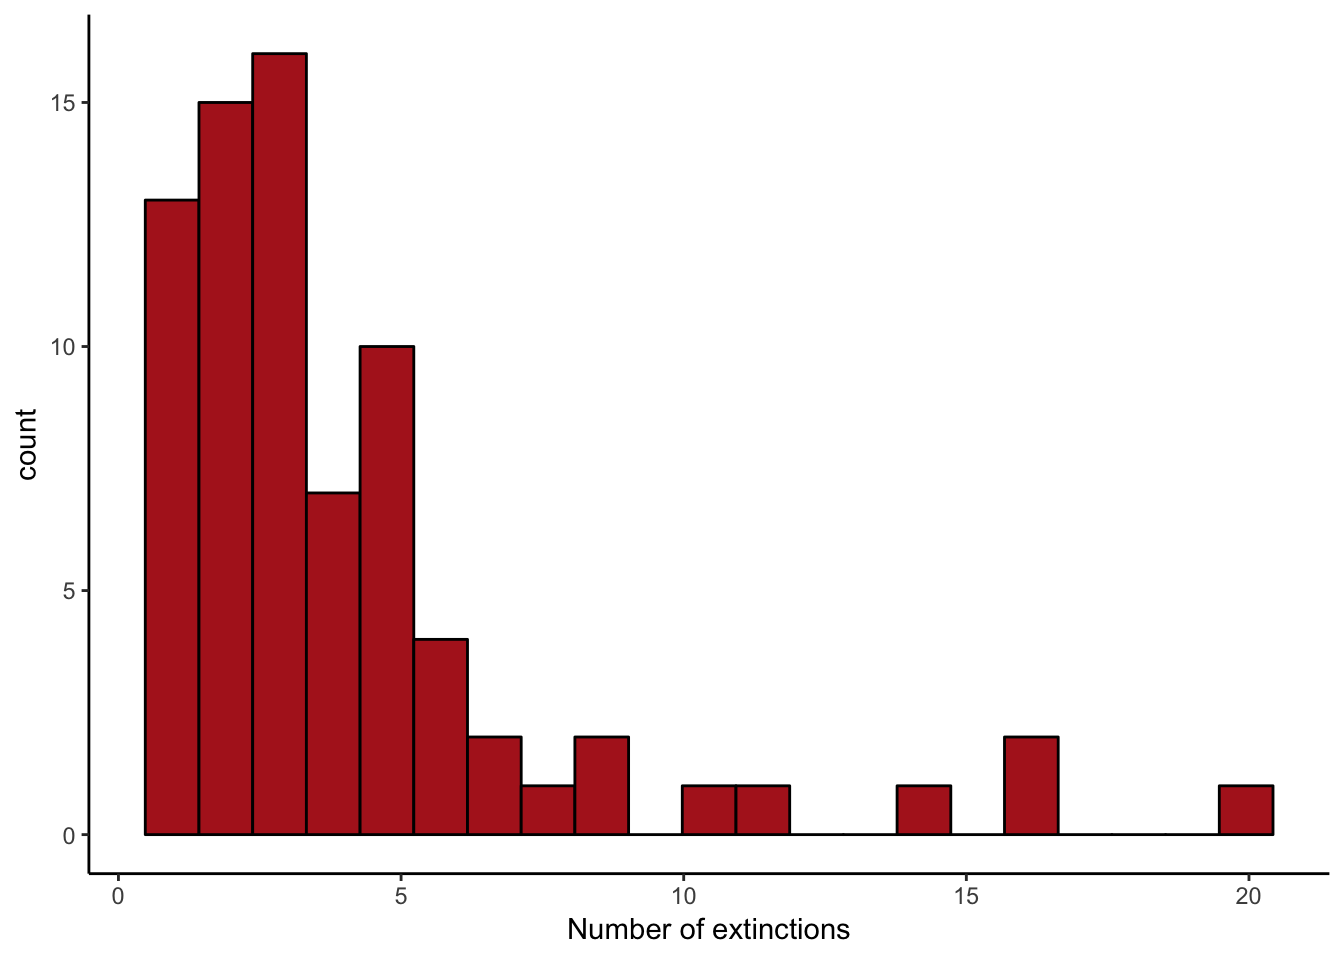
\includegraphics{index_files/figure-latex/unnamed-chunk-63-1.pdf}

Make a table of observed and expected frequencies, saving as a data
frame.

\begin{Shaded}
\begin{Highlighting}[]
\NormalTok{extinctFreq <-}\StringTok{ }\KeywordTok{data.frame}\NormalTok{(}\DataTypeTok{nExtinct =} \DecValTok{0}\OperatorTok{:}\DecValTok{20}\NormalTok{, }\DataTypeTok{obsFreq =} \KeywordTok{as.vector}\NormalTok{(extinctTable2), }
    \DataTypeTok{expFreq =}\NormalTok{ expectedFrequency)}
\NormalTok{extinctFreq}
\end{Highlighting}
\end{Shaded}

\begin{verbatim}
##    nExtinct obsFreq      expFreq
## 1         0       0 1.127730e+00
## 2         1      13 4.748338e+00
## 3         2      15 9.996501e+00
## 4         3      16 1.403018e+01
## 5         4       7 1.476861e+01
## 6         5      10 1.243672e+01
## 7         6       4 8.727524e+00
## 8         7       2 5.249639e+00
## 9         8       1 2.762968e+00
## 10        9       2 1.292616e+00
## 11       10       1 5.442596e-01
## 12       11       1 2.083290e-01
## 13       12       0 7.309790e-02
## 14       13       0 2.367543e-02
## 15       14       1 7.120431e-03
## 16       15       0 1.998718e-03
## 17       16       2 5.259783e-04
## 18       17       0 1.302733e-04
## 19       18       0 3.047328e-05
## 20       19       0 6.753081e-06
## 21       20       1 1.421701e-06
\end{verbatim}

The low expected frequencies will violate the assumptions of the
\(\chi^2\) test, so we will need to group categories. Create a new
variable that groups the extinctions into fewer categories (again, there
are many ways to do this, here I use the function \emph{cut}).

\begin{Shaded}
\begin{Highlighting}[]
\NormalTok{extinctFreq}\OperatorTok{$}\NormalTok{groups <-}\StringTok{ }\KeywordTok{cut}\NormalTok{(extinctFreq}\OperatorTok{$}\NormalTok{nExtinct, }
    \DataTypeTok{breaks =} \KeywordTok{c}\NormalTok{(}\DecValTok{0}\NormalTok{, }\DecValTok{2}\OperatorTok{:}\DecValTok{8}\NormalTok{, }\DecValTok{21}\NormalTok{), }\DataTypeTok{right =} \OtherTok{FALSE}\NormalTok{,}
    \DataTypeTok{labels =} \KeywordTok{c}\NormalTok{(}\StringTok{"0 or 1"}\NormalTok{,}\StringTok{"2"}\NormalTok{,}\StringTok{"3"}\NormalTok{,}\StringTok{"4"}\NormalTok{,}\StringTok{"5"}\NormalTok{,}\StringTok{"6"}\NormalTok{,}\StringTok{"7"}\NormalTok{,}\StringTok{"8 or more"}\NormalTok{))}
\NormalTok{extinctFreq}
\end{Highlighting}
\end{Shaded}

\begin{verbatim}
##    nExtinct obsFreq      expFreq    groups
## 1         0       0 1.127730e+00    0 or 1
## 2         1      13 4.748338e+00    0 or 1
## 3         2      15 9.996501e+00         2
## 4         3      16 1.403018e+01         3
## 5         4       7 1.476861e+01         4
## 6         5      10 1.243672e+01         5
## 7         6       4 8.727524e+00         6
## 8         7       2 5.249639e+00         7
## 9         8       1 2.762968e+00 8 or more
## 10        9       2 1.292616e+00 8 or more
## 11       10       1 5.442596e-01 8 or more
## 12       11       1 2.083290e-01 8 or more
## 13       12       0 7.309790e-02 8 or more
## 14       13       0 2.367543e-02 8 or more
## 15       14       1 7.120431e-03 8 or more
## 16       15       0 1.998718e-03 8 or more
## 17       16       2 5.259783e-04 8 or more
## 18       17       0 1.302733e-04 8 or more
## 19       18       0 3.047328e-05 8 or more
## 20       19       0 6.753081e-06 8 or more
## 21       20       1 1.421701e-06 8 or more
\end{verbatim}

Then sum up the observed and expected frequencies within the new
categories.

\begin{Shaded}
\begin{Highlighting}[]
\NormalTok{obsFreqGroup <-}\StringTok{ }\KeywordTok{tapply}\NormalTok{(extinctFreq}\OperatorTok{$}\NormalTok{obsFreq, extinctFreq}\OperatorTok{$}\NormalTok{groups, sum)}
\NormalTok{expFreqGroup <-}\StringTok{ }\KeywordTok{tapply}\NormalTok{(extinctFreq}\OperatorTok{$}\NormalTok{expFreq, extinctFreq}\OperatorTok{$}\NormalTok{groups, sum)}
\NormalTok{ObsVsExp =}\StringTok{ }\KeywordTok{data.frame}\NormalTok{(}\DataTypeTok{obs =}\NormalTok{ obsFreqGroup, }\DataTypeTok{exp =}\NormalTok{ expFreqGroup,}\DataTypeTok{group=} \KeywordTok{c}\NormalTok{(}\StringTok{"0 or 1"}\NormalTok{,}\StringTok{"2"}\NormalTok{,}\StringTok{"3"}\NormalTok{,}\StringTok{"4"}\NormalTok{,}\StringTok{"5"}\NormalTok{,}\StringTok{"6"}\NormalTok{,}\StringTok{"7"}\NormalTok{,}\StringTok{"8 or more"}\NormalTok{))}
\NormalTok{ObsVsExp}
\end{Highlighting}
\end{Shaded}

\begin{verbatim}
##           obs       exp     group
## 0 or 1     13  5.876068    0 or 1
## 2          15  9.996501         2
## 3          16 14.030177         3
## 4           7 14.768608         4
## 5          10 12.436722         5
## 6           4  8.727524         6
## 7           2  5.249639         7
## 8 or more   9  4.914760 8 or more
\end{verbatim}

The \emph{expected} frequency for the last category, ``8 or more'',
doesn't yet include the expected frequencies for the categories 21, 22,
23, and so on (remeber that we used a cut-off of 20 before!). However,
the expected frequencies must sum to 76. In the following, we
recalculate the expected frequency for the last group,
expFreqGroup{[}length(expFreqGroup){]}, as 76 minus the sum of the
expected frequencies for all the other groups.

\begin{Shaded}
\begin{Highlighting}[]
\NormalTok{expFreqGroup[}\KeywordTok{length}\NormalTok{(expFreqGroup)] =}\StringTok{ }\DecValTok{76} \OperatorTok{-}\StringTok{ }\KeywordTok{sum}\NormalTok{(expFreqGroup[}\DecValTok{1}\OperatorTok{:}\NormalTok{(}\KeywordTok{length}\NormalTok{(expFreqGroup)}\OperatorTok{-}\DecValTok{1}\NormalTok{)])}
\KeywordTok{data.frame}\NormalTok{(}\DataTypeTok{obs =}\NormalTok{ obsFreqGroup, }\DataTypeTok{exp =}\NormalTok{ expFreqGroup)}
\end{Highlighting}
\end{Shaded}

\begin{verbatim}
##           obs       exp
## 0 or 1     13  5.876068
## 2          15  9.996501
## 3          16 14.030177
## 4           7 14.768608
## 5          10 12.436722
## 6           4  8.727524
## 7           2  5.249639
## 8 or more   9  4.914761
\end{verbatim}

Finally, we are ready to carry out the \(\chi^2\) goodness-of-fit test.
R gives us a warning here because one of the expected frequencies is
less than 5. However, we have been careful to meet the assumptions of
the \(\chi^2\) test, so let's persevere. Once again, R doesn't know that
we have estimated a parameter from the data (the mean), so it won't use
the correct degrees of freedom when calculating the P-value. As before,
we need to grab the \(\chi^2\) value calculated by chisq.test and
recalculate \(P\) using the correct degrees of freedom. Since the number
of categories is now 8, the correct degrees of freedom is 8 - 1 - 1 = 6.

\begin{Shaded}
\begin{Highlighting}[]
\NormalTok{saveChiTest <-}\StringTok{ }\KeywordTok{chisq.test}\NormalTok{(obsFreqGroup, }\DataTypeTok{p =}\NormalTok{ expFreqGroup}\OperatorTok{/}\DecValTok{76}\NormalTok{)}
\end{Highlighting}
\end{Shaded}

\begin{verbatim}
## Warning in chisq.test(obsFreqGroup, p = expFreqGroup/76): Chi-squared
## approximation may be incorrect
\end{verbatim}

\begin{Shaded}
\begin{Highlighting}[]
\NormalTok{saveChiTest }
\end{Highlighting}
\end{Shaded}

\begin{verbatim}
## 
##  Chi-squared test for given probabilities
## 
## data:  obsFreqGroup
## X-squared = 23.95, df = 7, p-value = 0.001163
\end{verbatim}

\begin{Shaded}
\begin{Highlighting}[]
\CommentTok{# Wrong degrees of freedom, so wrong P-value!}

\NormalTok{pValue <-}\StringTok{ }\DecValTok{1} \OperatorTok{-}\StringTok{ }\KeywordTok{pchisq}\NormalTok{(saveChiTest}\OperatorTok{$}\NormalTok{statistic, }\DataTypeTok{df =} \DecValTok{6}\NormalTok{)}

\CommentTok{# correct P-value!}
\NormalTok{pValue }
\end{Highlighting}
\end{Shaded}

\begin{verbatim}
##    X-squared 
## 0.0005334919
\end{verbatim}

Finally, we can compare the expected and observed data in a histogramm.
One can clearly see that the fit is not very good.

\begin{Shaded}
\begin{Highlighting}[]
\NormalTok{df =}\StringTok{ }\KeywordTok{data.frame}\NormalTok{(}\DataTypeTok{x =} \DecValTok{0}\OperatorTok{:}\DecValTok{20}\NormalTok{,}\DataTypeTok{y =} \DecValTok{76}\OperatorTok{*}\KeywordTok{dpois}\NormalTok{(}\DecValTok{0}\OperatorTok{:}\DecValTok{20}\NormalTok{,meanExtinctions))}

\KeywordTok{ggplot}\NormalTok{(extinctData) }\OperatorTok{+}
\StringTok{  }\KeywordTok{geom_histogram}\NormalTok{(}\DataTypeTok{mapping=} \KeywordTok{aes}\NormalTok{(}\DataTypeTok{x =}\NormalTok{numberOfExtinctions),}\DataTypeTok{fill =} \StringTok{"firebrick"}\NormalTok{,}\DataTypeTok{color=}\StringTok{"black"}\NormalTok{,}\DataTypeTok{bins=}\DecValTok{21}\NormalTok{)}\OperatorTok{+}\StringTok{    }
\StringTok{  }\KeywordTok{labs}\NormalTok{ (}\DataTypeTok{x=}\StringTok{"Number of extinctions"}\NormalTok{) }\OperatorTok{+}\StringTok{ }
\StringTok{  }\KeywordTok{geom_line}\NormalTok{(}\DataTypeTok{data =}\NormalTok{ df, }\DataTypeTok{mapping =} \KeywordTok{aes}\NormalTok{(}\DataTypeTok{x =}\NormalTok{ x,}\DataTypeTok{y=}\NormalTok{y))}
\end{Highlighting}
\end{Shaded}

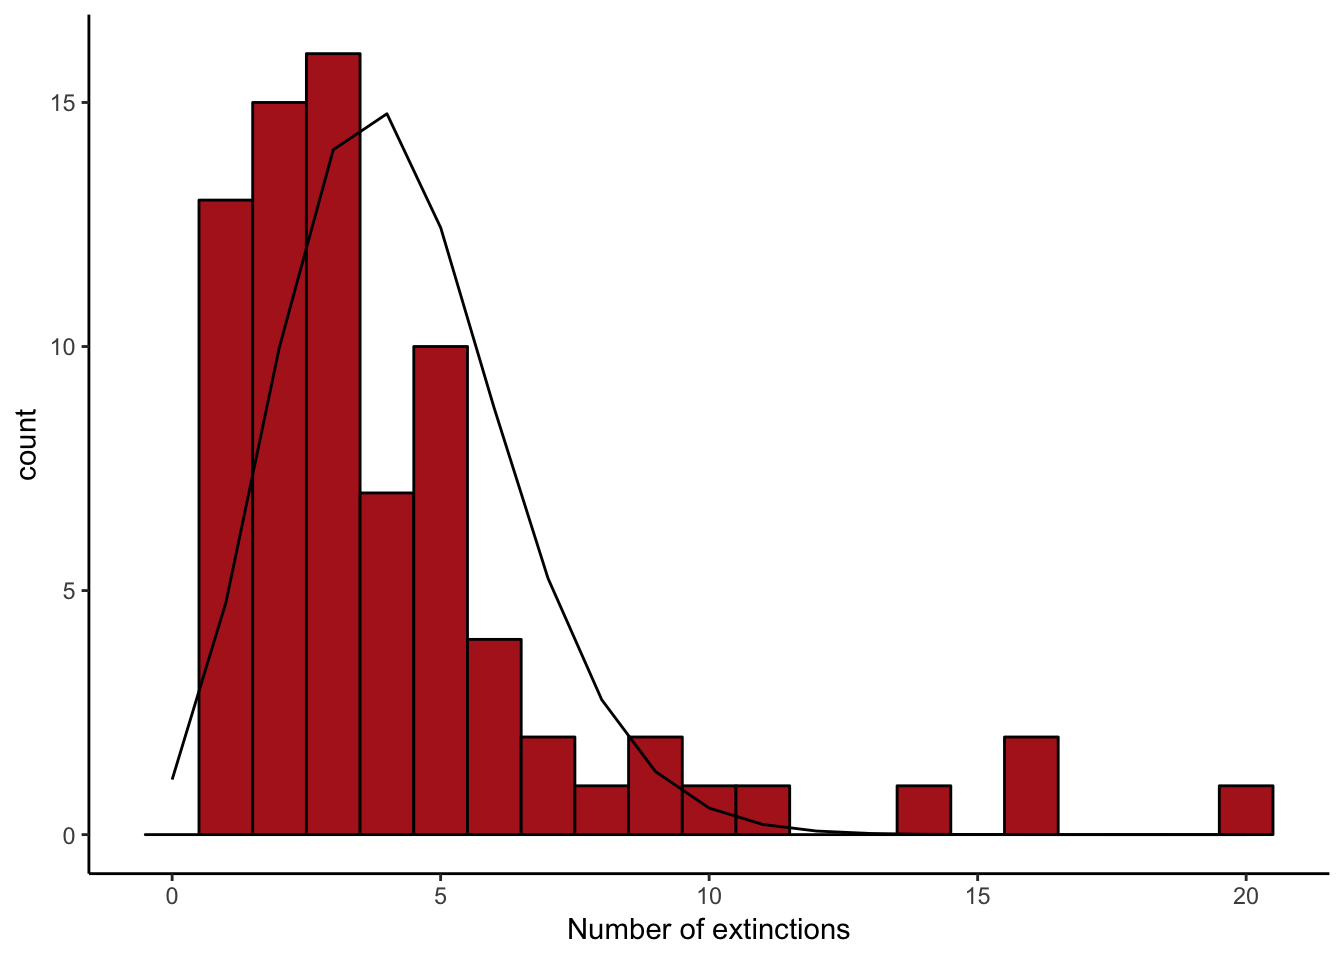
\includegraphics{index_files/figure-latex/unnamed-chunk-69-1.pdf} \#\#
t-test

\hypertarget{one-sample-t-test}{%
\subsubsection{One-sample t-test}\label{one-sample-t-test}}

We use a one-sample t-test to compare body temperature in a random
sample of people with the ``expected'' temperature 98.6 F.

Read and inspect the data:

\begin{Shaded}
\begin{Highlighting}[]
\NormalTok{heat <-}\StringTok{ }\KeywordTok{read.csv}\NormalTok{(}\KeywordTok{url}\NormalTok{(}\StringTok{"http://www.zoology.ubc.ca/~schluter/WhitlockSchluter/wp-content/data/chapter11/chap11e3Temperature.csv"}\NormalTok{))}
\KeywordTok{head}\NormalTok{(heat)}
\end{Highlighting}
\end{Shaded}

\begin{verbatim}
##   individual temperature
## 1          1        98.4
## 2          2        98.6
## 3          3        97.8
## 4          4        98.8
## 5          5        97.9
## 6          6        99.0
\end{verbatim}

\begin{Shaded}
\begin{Highlighting}[]
\KeywordTok{ggplot}\NormalTok{(}\DataTypeTok{data =}\NormalTok{ heat) }\OperatorTok{+}\StringTok{ }
\StringTok{  }\KeywordTok{geom_histogram}\NormalTok{(}\DataTypeTok{mapping =} \KeywordTok{aes}\NormalTok{(}\DataTypeTok{x =}\NormalTok{ temperature),}\DataTypeTok{fill =} \StringTok{"firebrick"}\NormalTok{,}\DataTypeTok{color=}\StringTok{"black"}\NormalTok{,}\DataTypeTok{bins=}\DecValTok{15}\NormalTok{) }\OperatorTok{+}\StringTok{ }
\StringTok{  }\KeywordTok{labs}\NormalTok{(}\DataTypeTok{x =} \StringTok{"Body temperature (degrees F)"}\NormalTok{,}\DataTypeTok{y =} \StringTok{"Frequency"}\NormalTok{, }\DataTypeTok{main =} \StringTok{""}\NormalTok{)}
\end{Highlighting}
\end{Shaded}

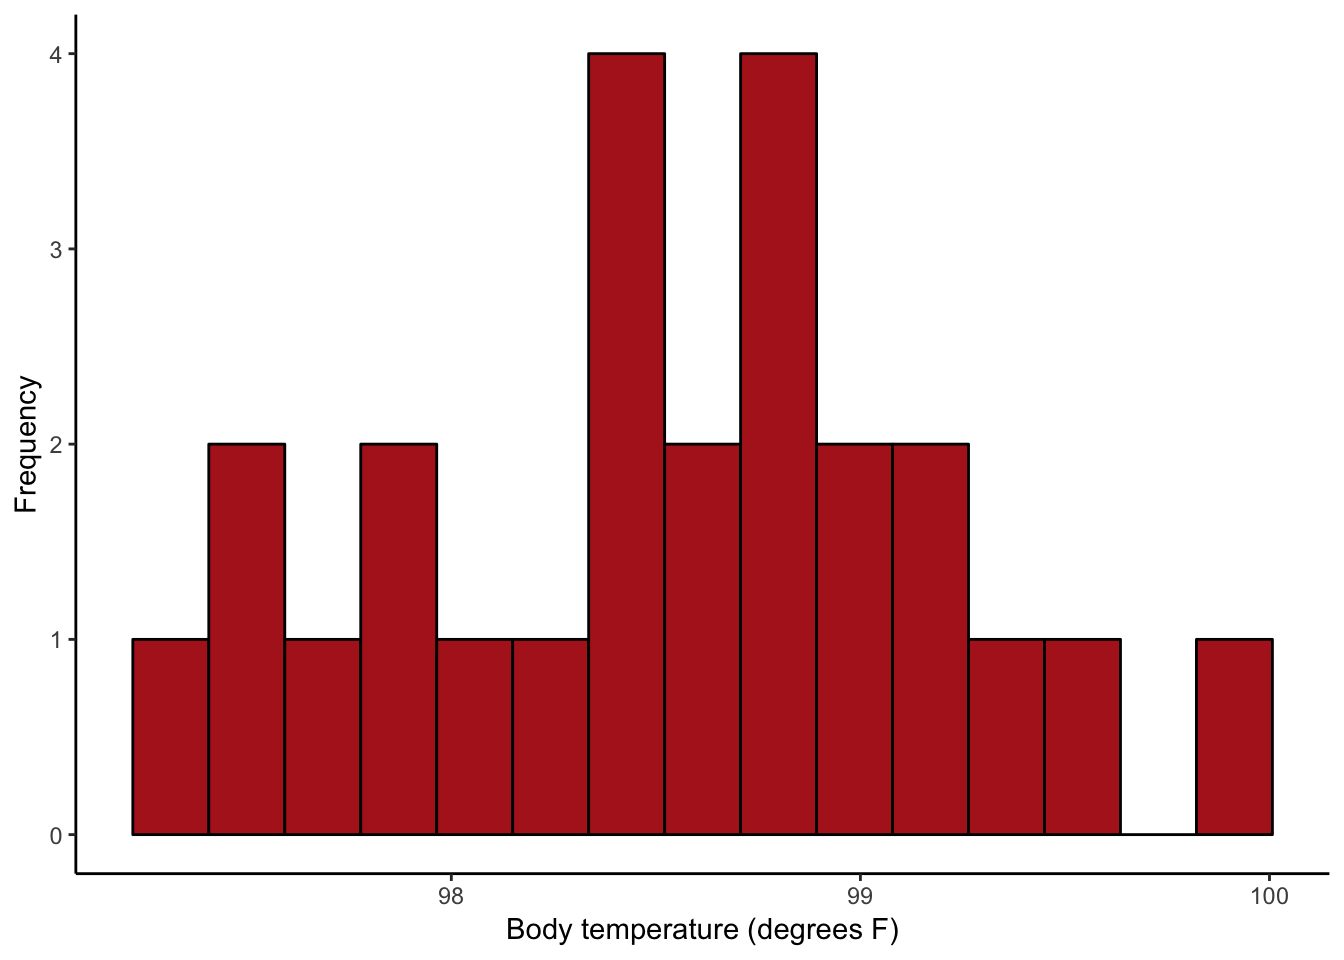
\includegraphics{index_files/figure-latex/unnamed-chunk-70-1.pdf}

A one-sample t-test can be calculate using the function t.test. The mu
argument gives the value stated in the null hypothesis. Let us first
transform the data into celsius using the formula to turn:
\[(X °F − 32) × 5/9 = Y °C\]

\begin{Shaded}
\begin{Highlighting}[]
\NormalTok{mu0 =}\StringTok{ }\NormalTok{(}\FloatTok{98.6}\DecValTok{-32}\NormalTok{)}\OperatorTok{*}\DecValTok{5}\OperatorTok{/}\DecValTok{9}

\NormalTok{heat =}\StringTok{ }\KeywordTok{mutate}\NormalTok{(heat,}\DataTypeTok{temperatureC =}\NormalTok{ (temperature}\DecValTok{-32}\NormalTok{) }\OperatorTok{*}\StringTok{ }\DecValTok{5}\OperatorTok{/}\DecValTok{9}\NormalTok{)}

\KeywordTok{ggplot}\NormalTok{(}\DataTypeTok{data =}\NormalTok{ heat) }\OperatorTok{+}\StringTok{ }
\StringTok{  }\KeywordTok{geom_histogram}\NormalTok{(}\DataTypeTok{mapping =} \KeywordTok{aes}\NormalTok{(}\DataTypeTok{x =}\NormalTok{ temperatureC),}\DataTypeTok{fill =} \StringTok{"firebrick"}\NormalTok{,}\DataTypeTok{color=}\StringTok{"black"}\NormalTok{,}\DataTypeTok{bins=}\DecValTok{15}\NormalTok{) }\OperatorTok{+}\StringTok{ }
\StringTok{  }\KeywordTok{labs}\NormalTok{(}\DataTypeTok{x =} \StringTok{"Body temperature (degrees C)"}\NormalTok{,}\DataTypeTok{y =} \StringTok{"Frequency"}\NormalTok{, }\DataTypeTok{main =} \StringTok{""}\NormalTok{)}
\end{Highlighting}
\end{Shaded}

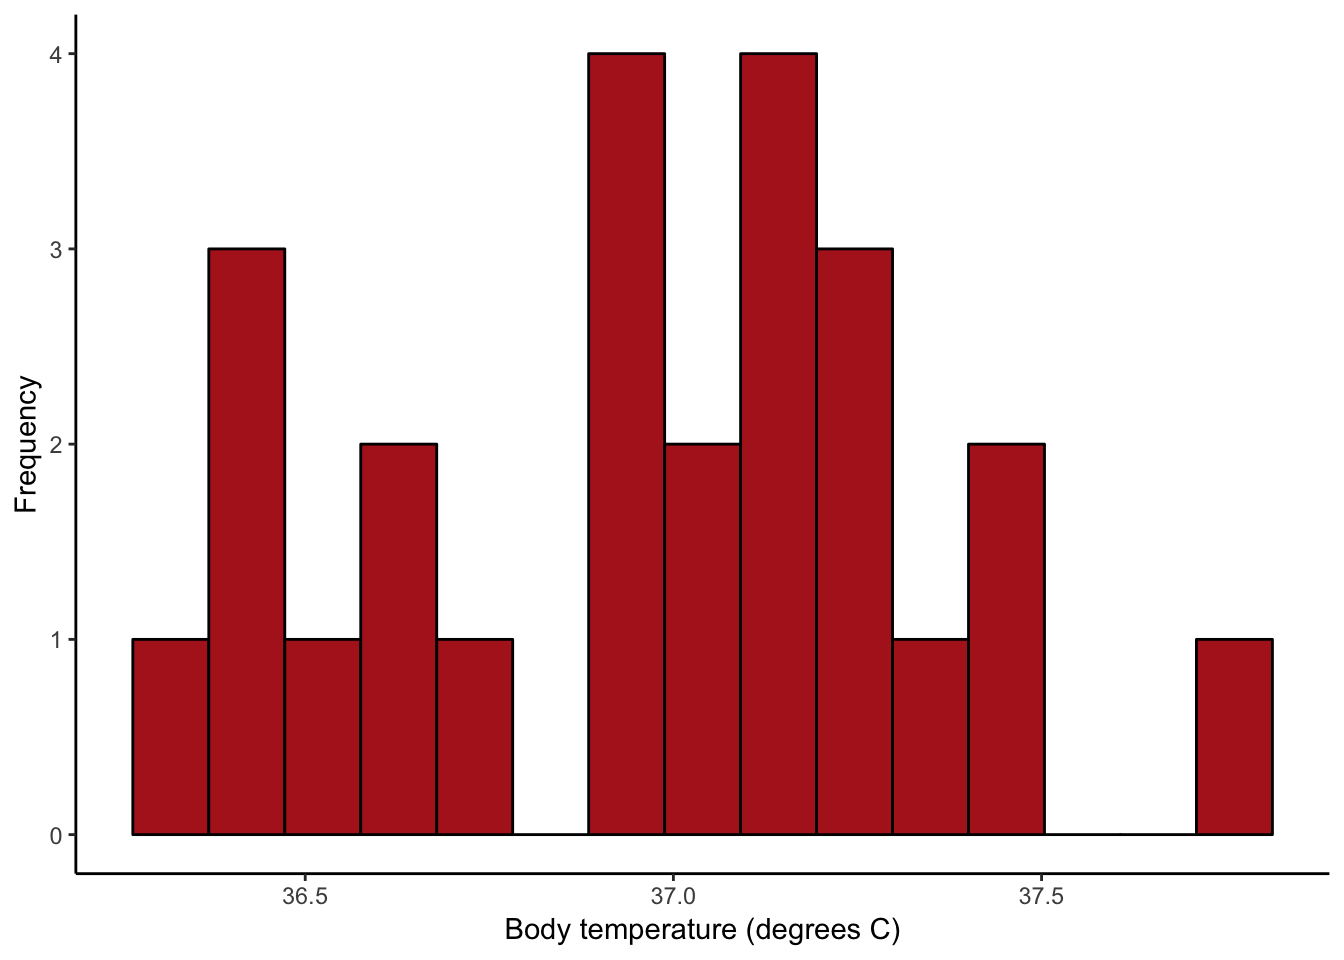
\includegraphics{index_files/figure-latex/unnamed-chunk-71-1.pdf}

\begin{Shaded}
\begin{Highlighting}[]
\KeywordTok{t.test}\NormalTok{(heat}\OperatorTok{$}\NormalTok{temperatureC, }\DataTypeTok{mu =}\NormalTok{ mu0)}
\end{Highlighting}
\end{Shaded}

\begin{verbatim}
## 
##  One Sample t-test
## 
## data:  heat$temperatureC
## t = -0.56065, df = 24, p-value = 0.5802
## alternative hypothesis: true mean is not equal to 37
## 95 percent confidence interval:
##  36.80235 37.11321
## sample estimates:
## mean of x 
##  36.95778
\end{verbatim}

\hypertarget{two-sample-t-test}{%
\subsubsection{Two-sample t-test}\label{two-sample-t-test}}

We compare horn length of live and dead (spiked) horned lizards.

\begin{Shaded}
\begin{Highlighting}[]
\NormalTok{lizard <-}\StringTok{ }\KeywordTok{read.csv}\NormalTok{(}\KeywordTok{url}\NormalTok{(}\StringTok{"http://www.zoology.ubc.ca/~schluter/WhitlockSchluter/wp-content/data/chapter12/chap12e3HornedLizards.csv"}\NormalTok{))}
\KeywordTok{head}\NormalTok{(lizard)}
\end{Highlighting}
\end{Shaded}

\begin{verbatim}
##   squamosalHornLength Survival
## 1                25.2   living
## 2                26.9   living
## 3                26.6   living
## 4                25.6   living
## 5                25.7   living
## 6                25.9   living
\end{verbatim}

Note that there is one missing value for the variable
``squamosalHornLength''. Everything is easier if we eliminate the row
with missing data.

\begin{Shaded}
\begin{Highlighting}[]
\NormalTok{lizard2 <-}\StringTok{ }\KeywordTok{na.omit}\NormalTok{(lizard)}
\KeywordTok{head}\NormalTok{(lizard2)}
\end{Highlighting}
\end{Shaded}

\begin{verbatim}
##   squamosalHornLength Survival
## 1                25.2   living
## 2                26.9   living
## 3                26.6   living
## 4                25.6   living
## 5                25.7   living
## 6                25.9   living
\end{verbatim}

\begin{Shaded}
\begin{Highlighting}[]
\KeywordTok{ggplot}\NormalTok{(}\DataTypeTok{data =}\NormalTok{ lizard2) }\OperatorTok{+}
\StringTok{  }\KeywordTok{geom_histogram}\NormalTok{(}\DataTypeTok{mapping =} \KeywordTok{aes}\NormalTok{(}\DataTypeTok{x =}\NormalTok{ squamosalHornLength ),}\DataTypeTok{fill =} \StringTok{"firebrick"}\NormalTok{,}\DataTypeTok{color=}\StringTok{"black"}\NormalTok{) }\OperatorTok{+}\StringTok{ }
\StringTok{  }\KeywordTok{facet_wrap}\NormalTok{( }\OperatorTok{~}\NormalTok{Survival,}\DataTypeTok{nrow=}\DecValTok{2}\NormalTok{) }\OperatorTok{+}\StringTok{ }
\StringTok{  }\KeywordTok{theme_classic}\NormalTok{() }
\end{Highlighting}
\end{Shaded}

\begin{verbatim}
## `stat_bin()` using `bins = 30`. Pick better value with `binwidth`.
\end{verbatim}

\includegraphics{index_files/figure-latex/unnamed-chunk-74-1.pdf}

A two-sample t-test of the difference between two means can be carried
out with t.test by using a formula, asking if squamosalHornLength is
predicted by Survival, and specifying that the variables are in the data
frame lizard.

\begin{Shaded}
\begin{Highlighting}[]
\KeywordTok{t.test}\NormalTok{(squamosalHornLength }\OperatorTok{~}\StringTok{ }\NormalTok{Survival, }\DataTypeTok{data =}\NormalTok{ lizard)}
\end{Highlighting}
\end{Shaded}

\begin{verbatim}
## 
##  Welch Two Sample t-test
## 
## data:  squamosalHornLength by Survival
## t = -4.2634, df = 40.372, p-value = 0.0001178
## alternative hypothesis: true difference in means is not equal to 0
## 95 percent confidence interval:
##  -3.381912 -1.207092
## sample estimates:
## mean in group killed mean in group living 
##             21.98667             24.28117
\end{verbatim}

The same reuslt could be achieved with

\begin{Shaded}
\begin{Highlighting}[]
\KeywordTok{t.test}\NormalTok{(lizard}\OperatorTok{$}\NormalTok{squamosalHornLength[lizard}\OperatorTok{$}\NormalTok{Survival}\OperatorTok{==}\StringTok{"killed"}\NormalTok{], lizard}\OperatorTok{$}\NormalTok{squamosalHornLength[lizard}\OperatorTok{$}\NormalTok{Survival}\OperatorTok{==}\StringTok{"living"}\NormalTok{])}
\end{Highlighting}
\end{Shaded}

\begin{verbatim}
## 
##  Welch Two Sample t-test
## 
## data:  lizard$squamosalHornLength[lizard$Survival == "killed"] and lizard$squamosalHornLength[lizard$Survival == "living"]
## t = -4.2634, df = 40.372, p-value = 0.0001178
## alternative hypothesis: true difference in means is not equal to 0
## 95 percent confidence interval:
##  -3.381912 -1.207092
## sample estimates:
## mean of x mean of y 
##  21.98667  24.28117
\end{verbatim}

The output of t.test includes the 95\% confidence interval for the
difference between means. Add \$confint after calling the function to
get R to report only the confidence interval. The formula in the
following command tells R to compare squamosalHornLength between the two
groups indicated by Survival.

\begin{Shaded}
\begin{Highlighting}[]
\KeywordTok{t.test}\NormalTok{(squamosalHornLength }\OperatorTok{~}\StringTok{ }\NormalTok{Survival, }\DataTypeTok{data =}\NormalTok{ lizard)}\OperatorTok{$}\NormalTok{conf.int}
\end{Highlighting}
\end{Shaded}

\begin{verbatim}
## [1] -3.381912 -1.207092
## attr(,"conf.level")
## [1] 0.95
\end{verbatim}

*Note: R has used the Welch two sample t-test here. If we want to force
R to use the standrad t.test we set a parameter specifiying this:

\begin{Shaded}
\begin{Highlighting}[]
\KeywordTok{t.test}\NormalTok{(squamosalHornLength }\OperatorTok{~}\StringTok{ }\NormalTok{Survival, }\DataTypeTok{data =}\NormalTok{ lizard,}\DataTypeTok{var.equal =} \OtherTok{TRUE}\NormalTok{)}
\end{Highlighting}
\end{Shaded}

\begin{verbatim}
## 
##  Two Sample t-test
## 
## data:  squamosalHornLength by Survival
## t = -4.3494, df = 182, p-value = 2.27e-05
## alternative hypothesis: true difference in means is not equal to 0
## 95 percent confidence interval:
##  -3.335402 -1.253602
## sample estimates:
## mean in group killed mean in group living 
##             21.98667             24.28117
\end{verbatim}

\hypertarget{deviations-from-normailty}{%
\section{Deviations from Normailty}\label{deviations-from-normailty}}

\hypertarget{qq-plots-and-transformations}{%
\subsection{QQ Plots and
Transformations}\label{qq-plots-and-transformations}}

We investigate the ratio of biomass between marine reserves and
non-reserve control areas.

\begin{Shaded}
\begin{Highlighting}[]
\NormalTok{marine <-}\StringTok{ }\KeywordTok{read.csv}\NormalTok{(}\KeywordTok{url}\NormalTok{(}\StringTok{"http://www.zoology.ubc.ca/~schluter/WhitlockSchluter/wp-content/data/chapter13/chap13e1MarineReserve.csv"}\NormalTok{))}
\KeywordTok{head}\NormalTok{(marine)}
\end{Highlighting}
\end{Shaded}

\begin{verbatim}
##   biomassRatio
## 1         1.34
## 2         1.96
## 3         2.49
## 4         1.27
## 5         1.19
## 6         1.15
\end{verbatim}

\begin{Shaded}
\begin{Highlighting}[]
\KeywordTok{ggplot}\NormalTok{(}\DataTypeTok{data =}\NormalTok{ marine) }\OperatorTok{+}
\StringTok{  }\KeywordTok{geom_histogram}\NormalTok{(}\DataTypeTok{mapping =} \KeywordTok{aes}\NormalTok{(}\DataTypeTok{x =}\NormalTok{ biomassRatio))}
\end{Highlighting}
\end{Shaded}

\begin{verbatim}
## `stat_bin()` using `bins = 30`. Pick better value with `binwidth`.
\end{verbatim}

\includegraphics{index_files/figure-latex/unnamed-chunk-79-1.pdf} Normal
quantile plot of biomass ratio data.

\begin{Shaded}
\begin{Highlighting}[]
\KeywordTok{library}\NormalTok{(car)}
\end{Highlighting}
\end{Shaded}

\begin{verbatim}
## 
## Attaching package: 'car'
\end{verbatim}

\begin{verbatim}
## The following object is masked from 'package:dplyr':
## 
##     recode
\end{verbatim}

\begin{verbatim}
## The following object is masked from 'package:purrr':
## 
##     some
\end{verbatim}

\begin{Shaded}
\begin{Highlighting}[]
\KeywordTok{qqPlot}\NormalTok{(marine}\OperatorTok{$}\NormalTok{biomassRatio, }\DataTypeTok{distribution =} \StringTok{"norm"}\NormalTok{)}
\end{Highlighting}
\end{Shaded}

\includegraphics{index_files/figure-latex/unnamed-chunk-80-1.pdf}

The function log() takes the natural logarithm of all the elements of a
vector or variable. The following command puts the results into a new
variable in the same data frame, marine.

\begin{Shaded}
\begin{Highlighting}[]
\NormalTok{marine =}\StringTok{ }\KeywordTok{mutate}\NormalTok{(marine,}\DataTypeTok{logBiomassRatio =}  \KeywordTok{log}\NormalTok{(biomassRatio))}
\end{Highlighting}
\end{Shaded}

Histogram and QQ-Plot of the log-transformed marine biomass ratio.

\begin{Shaded}
\begin{Highlighting}[]
\KeywordTok{ggplot}\NormalTok{(}\DataTypeTok{data =}\NormalTok{ marine) }\OperatorTok{+}
\StringTok{  }\KeywordTok{geom_histogram}\NormalTok{(}\DataTypeTok{mapping =} \KeywordTok{aes}\NormalTok{(}\DataTypeTok{x =}\NormalTok{ logBiomassRatio),}\DataTypeTok{col=}\StringTok{"black"}\NormalTok{,}\DataTypeTok{fill=}\StringTok{"darkred"}\NormalTok{)}
\end{Highlighting}
\end{Shaded}

\begin{verbatim}
## `stat_bin()` using `bins = 30`. Pick better value with `binwidth`.
\end{verbatim}

\includegraphics{index_files/figure-latex/unnamed-chunk-82-1.pdf}

\begin{Shaded}
\begin{Highlighting}[]
\KeywordTok{qqPlot}\NormalTok{(marine}\OperatorTok{$}\NormalTok{logBiomassRatio, }\DataTypeTok{distribution =} \StringTok{"norm"}\NormalTok{)}
\end{Highlighting}
\end{Shaded}

\includegraphics{index_files/figure-latex/unnamed-chunk-82-2.pdf}

95\% confidence interval of the mean using the log-transformed data.

\begin{Shaded}
\begin{Highlighting}[]
\KeywordTok{t.test}\NormalTok{(marine}\OperatorTok{$}\NormalTok{logBiomassRatio)}\OperatorTok{$}\NormalTok{conf.int}
\end{Highlighting}
\end{Shaded}

\begin{verbatim}
## [1] 0.3470180 0.6112365
## attr(,"conf.level")
## [1] 0.95
\end{verbatim}

Back-transform lower and upper limits of confidence interval (exp is the
inverse of the log function).

\begin{Shaded}
\begin{Highlighting}[]
\NormalTok{conf.int =}\StringTok{ }\KeywordTok{exp}\NormalTok{(}\KeywordTok{t.test}\NormalTok{(marine}\OperatorTok{$}\NormalTok{logBiomassRatio)}\OperatorTok{$}\NormalTok{conf.int )}
\NormalTok{meanBiomassRatio =}\StringTok{ }\KeywordTok{mean}\NormalTok{(marine}\OperatorTok{$}\NormalTok{biomassRatio)}

\KeywordTok{ggplot}\NormalTok{(}\DataTypeTok{data =}\NormalTok{ marine) }\OperatorTok{+}\StringTok{ }
\StringTok{  }\KeywordTok{geom_histogram}\NormalTok{(}\DataTypeTok{mapping=} \KeywordTok{aes}\NormalTok{(}\DataTypeTok{x =}\NormalTok{ biomassRatio),}\DataTypeTok{col=}\StringTok{"black"}\NormalTok{,}\DataTypeTok{fill=}\StringTok{"darkred"}\NormalTok{) }\OperatorTok{+}\StringTok{ }
\StringTok{  }\KeywordTok{geom_vline}\NormalTok{(}\DataTypeTok{xintercept =}\NormalTok{ conf.int)}\OperatorTok{+}\StringTok{ }
\StringTok{  }\KeywordTok{geom_vline}\NormalTok{(}\DataTypeTok{xintercept =}\NormalTok{ meanBiomassRatio,}\DataTypeTok{lwd=}\DecValTok{2}\NormalTok{)}
\end{Highlighting}
\end{Shaded}

\begin{verbatim}
## `stat_bin()` using `bins = 30`. Pick better value with `binwidth`.
\end{verbatim}

\includegraphics{index_files/figure-latex/unnamed-chunk-84-1.pdf}

\hypertarget{non-parametric-alternatives}{%
\subsection{Non-Parametric
Alternatives}\label{non-parametric-alternatives}}

We use the Wilcoxon rank-sum test (equivalent to the Mann-Whitney
U-test) comparing times to mating (in hours) of starved and fed female
sagebrush crickets. We also apply the permutation test to the same data.

Read and inspect data:

\begin{Shaded}
\begin{Highlighting}[]
\NormalTok{cannibalism <-}\StringTok{ }\KeywordTok{read.csv}\NormalTok{(}\KeywordTok{url}\NormalTok{(}\StringTok{"http://www.zoology.ubc.ca/~schluter/WhitlockSchluter/wp-content/data/chapter13/chap13e5SagebrushCrickets.csv"}\NormalTok{))}
\KeywordTok{head}\NormalTok{(cannibalism)}
\end{Highlighting}
\end{Shaded}

\begin{verbatim}
##   feedingStatus timeToMating
## 1       starved          1.9
## 2       starved          2.1
## 3       starved          3.8
## 4       starved          9.0
## 5       starved          9.6
## 6       starved         13.0
\end{verbatim}

\begin{Shaded}
\begin{Highlighting}[]
\KeywordTok{ggplot}\NormalTok{(}\DataTypeTok{data =}\NormalTok{ cannibalism) }\OperatorTok{+}
\StringTok{  }\KeywordTok{geom_histogram}\NormalTok{(}\DataTypeTok{mapping =} \KeywordTok{aes}\NormalTok{(}\DataTypeTok{x =}\NormalTok{ timeToMating ),}\DataTypeTok{bins=}\DecValTok{12}\NormalTok{,}\DataTypeTok{color=}\StringTok{"black"}\NormalTok{,}\DataTypeTok{fill=}\StringTok{"darkred"}\NormalTok{) }\OperatorTok{+}\StringTok{ }
\StringTok{  }\KeywordTok{facet_wrap}\NormalTok{( }\OperatorTok{~}\NormalTok{feedingStatus,}\DataTypeTok{nrow=}\DecValTok{2}\NormalTok{) }\OperatorTok{+}\StringTok{ }
\StringTok{  }\KeywordTok{theme_classic}\NormalTok{() }
\end{Highlighting}
\end{Shaded}

\includegraphics{index_files/figure-latex/unnamed-chunk-86-1.pdf}

We perfrom the Wilcoxon rank-sum test (equivalent to Mann-Whitney
U-test)

\begin{Shaded}
\begin{Highlighting}[]
\KeywordTok{wilcox.test}\NormalTok{(timeToMating }\OperatorTok{~}\StringTok{ }\NormalTok{feedingStatus, }\DataTypeTok{data =}\NormalTok{ cannibalism)}
\end{Highlighting}
\end{Shaded}

\begin{verbatim}
## 
##  Wilcoxon rank sum test
## 
## data:  timeToMating by feedingStatus
## W = 88, p-value = 0.3607
## alternative hypothesis: true location shift is not equal to 0
\end{verbatim}

\hypertarget{permutation-test}{%
\subsection{Permutation Test}\label{permutation-test}}

We use a permutation test of the difference between mean time to mating
of starved and fed crickets.We begin by calculating the observed
difference between means (starved minus fed). The difference is
-18.25734 in this data set.

\begin{Shaded}
\begin{Highlighting}[]
\CommentTok{# tapply is another way to calcualte the means of time to mating}
\CommentTok{# for each feeding status seperatly}

\NormalTok{cricketMeans <-}\StringTok{ }\KeywordTok{tapply}\NormalTok{(cannibalism}\OperatorTok{$}\NormalTok{timeToMating, cannibalism}\OperatorTok{$}\NormalTok{feedingStatus, mean)}

\NormalTok{cricketMeans}
\end{Highlighting}
\end{Shaded}

\begin{verbatim}
##      fed  starved 
## 35.98462 17.72727
\end{verbatim}

\begin{Shaded}
\begin{Highlighting}[]
\NormalTok{diffMeans <-}\StringTok{ }\NormalTok{cricketMeans[}\DecValTok{2}\NormalTok{] }\OperatorTok{-}\StringTok{ }\NormalTok{cricketMeans[}\DecValTok{1}\NormalTok{]}
\NormalTok{diffMeans}
\end{Highlighting}
\end{Shaded}

\begin{verbatim}
##   starved 
## -18.25734
\end{verbatim}

We choose to perform 1000 permutations.

\begin{Shaded}
\begin{Highlighting}[]
\NormalTok{nPerm <-}\StringTok{ }\DecValTok{10000}
\end{Highlighting}
\end{Shaded}

The following code implements aloop to permute the data many times
(determined by nperm, investigate the function sample to see what it
does). In the loop, i is just a counter that goes from 1 to nPerm by 1;
each permuted difference is saved in the permResult.

\begin{Shaded}
\begin{Highlighting}[]
\NormalTok{permResult <-}\StringTok{ }\KeywordTok{vector}\NormalTok{() }\CommentTok{# initializes}
\ControlFlowTok{for}\NormalTok{(i }\ControlFlowTok{in} \DecValTok{1}\OperatorTok{:}\NormalTok{nPerm)\{}
    \CommentTok{# step 1: permute the times to mating}
\NormalTok{    permSample <-}\StringTok{ }\KeywordTok{sample}\NormalTok{(cannibalism}\OperatorTok{$}\NormalTok{timeToMating, }\DataTypeTok{replace =} \OtherTok{FALSE}\NormalTok{)}
    \CommentTok{# step 2: calculate difference betweeen means}
\NormalTok{    permMeans <-}\StringTok{ }\KeywordTok{tapply}\NormalTok{(permSample, cannibalism}\OperatorTok{$}\NormalTok{feedingStatus, mean)}
\NormalTok{    permResult[i] <-}\StringTok{ }\NormalTok{permMeans[}\DecValTok{2}\NormalTok{] }\OperatorTok{-}\StringTok{ }\NormalTok{permMeans[}\DecValTok{1}\NormalTok{]}
\NormalTok{\}}
\end{Highlighting}
\end{Shaded}

Plot null distribution based on the permuted differences.

\begin{Shaded}
\begin{Highlighting}[]
\KeywordTok{hist}\NormalTok{(permResult, }\DataTypeTok{right =} \OtherTok{FALSE}\NormalTok{, }\DataTypeTok{breaks =} \DecValTok{100}\NormalTok{,}\DataTypeTok{col=}\StringTok{"darkred"}\NormalTok{)}
\end{Highlighting}
\end{Shaded}

\includegraphics{index_files/figure-latex/unnamed-chunk-91-1.pdf}

Use the null distribution to calculate an approximate P-value. This is
the twice the proportion of the permuted means that fall below the
observed difference in means, diffMeans (-18.25734 in this example). The
following code calculates the number of permuted means falling below
diffMeans.

\begin{Shaded}
\begin{Highlighting}[]
\KeywordTok{sum}\NormalTok{(}\KeywordTok{as.numeric}\NormalTok{(permResult }\OperatorTok{<=}\StringTok{ }\NormalTok{diffMeans))}
\end{Highlighting}
\end{Shaded}

\begin{verbatim}
## [1] 650
\end{verbatim}

These commands obtain the fraction of permuted means falling below
diffMeans.

\begin{Shaded}
\begin{Highlighting}[]
\KeywordTok{sum}\NormalTok{(}\KeywordTok{as.numeric}\NormalTok{(permResult }\OperatorTok{<=}\StringTok{ }\NormalTok{diffMeans)) }\OperatorTok{/}\StringTok{ }\NormalTok{nPerm}
\end{Highlighting}
\end{Shaded}

\begin{verbatim}
## [1] 0.065
\end{verbatim}

Finally, multiply by 2 to get the P-value for a two-sided test.

\begin{Shaded}
\begin{Highlighting}[]
\DecValTok{2} \OperatorTok{*}\StringTok{ }\NormalTok{( }\KeywordTok{sum}\NormalTok{(}\KeywordTok{as.numeric}\NormalTok{(permResult }\OperatorTok{<=}\StringTok{ }\NormalTok{diffMeans)) }\OperatorTok{/}\StringTok{ }\NormalTok{nPerm )}
\end{Highlighting}
\end{Shaded}

\begin{verbatim}
## [1] 0.13
\end{verbatim}

We can illustrate the permutaed differences and add the observed
difference on to show the outcome of our test: the birght red colored
bars indicate the proportion of permutation results that yielded a more
exterme results as the on observed.

\begin{Shaded}
\begin{Highlighting}[]
\KeywordTok{hist}\NormalTok{(permResult[permResult}\OperatorTok{>}\NormalTok{diffMeans],}\DataTypeTok{breaks=}\KeywordTok{seq}\NormalTok{(}\OperatorTok{-}\DecValTok{40}\NormalTok{,}\DecValTok{40}\NormalTok{,}\DataTypeTok{by=}\DecValTok{1}\NormalTok{),}\DataTypeTok{col=}\StringTok{"darkred"}\NormalTok{,}\DataTypeTok{main=}\StringTok{""}\NormalTok{)}
\KeywordTok{hist}\NormalTok{(permResult[permResult}\OperatorTok{<=}\NormalTok{diffMeans],}\DataTypeTok{breaks=}\KeywordTok{seq}\NormalTok{(}\OperatorTok{-}\DecValTok{40}\NormalTok{,}\DecValTok{40}\NormalTok{,}\DataTypeTok{by=}\DecValTok{1}\NormalTok{),}\DataTypeTok{add=}\NormalTok{T,}\DataTypeTok{col=}\StringTok{"red"}\NormalTok{)}
\KeywordTok{abline}\NormalTok{(}\DataTypeTok{v =}\NormalTok{ diffMeans,}\DataTypeTok{col=}\StringTok{"red"}\NormalTok{,}\DataTypeTok{lwd=}\DecValTok{2}\NormalTok{)}
\end{Highlighting}
\end{Shaded}

\includegraphics{index_files/figure-latex/unnamed-chunk-95-1.pdf}

\hypertarget{anova}{%
\section{ANOVA}\label{anova}}

\hypertarget{one-way-anova}{%
\subsection{One way ANOVA}\label{one-way-anova}}

We compare the phase shift in the circadian rhythm of melatonin
production in participants given alternative light treatments.

Read and inspect the data.

\begin{Shaded}
\begin{Highlighting}[]
\NormalTok{circadian <-}\StringTok{ }\KeywordTok{read.csv}\NormalTok{(}\KeywordTok{url}\NormalTok{(}\StringTok{"http://www.zoology.ubc.ca/~schluter/WhitlockSchluter/wp-content/data/chapter15/chap15e1KneesWhoSayNight.csv"}\NormalTok{))}
\end{Highlighting}
\end{Shaded}

Set the preferred ordering of groups in tables and graphs.

\begin{Shaded}
\begin{Highlighting}[]
\NormalTok{circadian}\OperatorTok{$}\NormalTok{treatment <-}\StringTok{ }\KeywordTok{factor}\NormalTok{(circadian}\OperatorTok{$}\NormalTok{treatment, }
    \DataTypeTok{levels =} \KeywordTok{c}\NormalTok{(}\StringTok{"control"}\NormalTok{, }\StringTok{"knee"}\NormalTok{, }\StringTok{"eyes"}\NormalTok{)) }



\NormalTok{meanShift <-}\StringTok{ }\KeywordTok{tapply}\NormalTok{(circadian}\OperatorTok{$}\NormalTok{shift, circadian}\OperatorTok{$}\NormalTok{treatment, mean)}
\NormalTok{sdevShift <-}\StringTok{ }\KeywordTok{tapply}\NormalTok{(circadian}\OperatorTok{$}\NormalTok{shift, circadian}\OperatorTok{$}\NormalTok{treatment, sd)}
\NormalTok{n         <-}\StringTok{ }\KeywordTok{tapply}\NormalTok{(circadian}\OperatorTok{$}\NormalTok{shift, circadian}\OperatorTok{$}\NormalTok{treatment, length)}
\NormalTok{mean_SD =}\KeywordTok{data.frame}\NormalTok{(}\DataTypeTok{mean =}\NormalTok{ meanShift, }\DataTypeTok{std.dev =}\NormalTok{ sdevShift, }\DataTypeTok{n =}\NormalTok{ n,}\DataTypeTok{treatment =} \KeywordTok{c}\NormalTok{(}\StringTok{"control"}\NormalTok{, }\StringTok{"knee"}\NormalTok{, }\StringTok{"eyes"}\NormalTok{))}
\end{Highlighting}
\end{Shaded}

We plot the data showing the raw data points as well as the mean
(including error bars shwoing one standard error in each direction).

\begin{Shaded}
\begin{Highlighting}[]
\KeywordTok{ggplot}\NormalTok{(}\DataTypeTok{data =}\NormalTok{ circadian) }\OperatorTok{+}
\StringTok{  }\KeywordTok{geom_jitter}\NormalTok{(}\DataTypeTok{mapping =} \KeywordTok{aes}\NormalTok{(}\DataTypeTok{x =}\NormalTok{ treatment,}\DataTypeTok{y=}\NormalTok{shift),}\DataTypeTok{width=}\FloatTok{0.1}\NormalTok{) }\OperatorTok{+}\StringTok{ }
\StringTok{  }\KeywordTok{geom_errorbar}\NormalTok{(}\DataTypeTok{data =}\NormalTok{ mean_SD,}\DataTypeTok{mapping =} \KeywordTok{aes}\NormalTok{(}\DataTypeTok{x =}\NormalTok{ treatment,}\DataTypeTok{ymin=}\NormalTok{meanShift}\OperatorTok{-}\NormalTok{sdevShift}\OperatorTok{/}\KeywordTok{sqrt}\NormalTok{(n), }\DataTypeTok{ymax=}\NormalTok{meanShift}\OperatorTok{+}\NormalTok{sdevShift}\OperatorTok{/}\KeywordTok{sqrt}\NormalTok{(n)), }\DataTypeTok{width=}\NormalTok{.}\DecValTok{1}\NormalTok{,}\DataTypeTok{color=}\StringTok{"red"}\NormalTok{) }\OperatorTok{+}\StringTok{ }
\StringTok{  }\KeywordTok{geom_point}\NormalTok{(}\DataTypeTok{data =}\NormalTok{ mean_SD,}\DataTypeTok{mapping =} \KeywordTok{aes}\NormalTok{(}\DataTypeTok{x =}\NormalTok{ treatment,}\DataTypeTok{y=}\NormalTok{meanShift),}\DataTypeTok{color=}\StringTok{"red"}\NormalTok{)}
\end{Highlighting}
\end{Shaded}

\includegraphics{index_files/figure-latex/unnamed-chunk-98-1.pdf}

The first step involves fitting the ANOVA model to the data using lm
(``lm'' stands for ``linear model'', of which ANOVA is one type). Then
we use the command anova to assemble the ANOVA table.

\begin{Shaded}
\begin{Highlighting}[]
\NormalTok{circadianAnova <-}\StringTok{ }\KeywordTok{lm}\NormalTok{(shift }\OperatorTok{~}\StringTok{ }\NormalTok{treatment, }\DataTypeTok{data =}\NormalTok{ circadian)}
\KeywordTok{anova}\NormalTok{(circadianAnova)}
\end{Highlighting}
\end{Shaded}

\begin{verbatim}
## Analysis of Variance Table
## 
## Response: shift
##           Df Sum Sq Mean Sq F value   Pr(>F)   
## treatment  2 7.2245  3.6122  7.2894 0.004472 **
## Residuals 19 9.4153  0.4955                    
## ---
## Signif. codes:  0 '***' 0.001 '**' 0.01 '*' 0.05 '.' 0.1 ' ' 1
\end{verbatim}

R2 indicating the fraction of variation in the response variable
``explained'' by treatment. This is again done in two steps. The first
step calculates a bunch of useful quantities from the ANOVA model object
previously created with a lm command. The second step shows the R2
value.

\begin{Shaded}
\begin{Highlighting}[]
\NormalTok{circadianAnovaSummary <-}\StringTok{ }\KeywordTok{summary}\NormalTok{(circadianAnova)}
\NormalTok{circadianAnovaSummary}\OperatorTok{$}\NormalTok{r.squared}
\end{Highlighting}
\end{Shaded}

\begin{verbatim}
## [1] 0.4341684
\end{verbatim}

\hypertarget{two-way-anova}{%
\subsection{Two way ANOVA}\label{two-way-anova}}

Analyze data from a factorial experiment investigating the effects of
herbivore presence, height above low tide, and the interaction between
these factors, on abundance of a red intertidal alga using two-factor
ANOVA.

Read and inspect the data.

\begin{Shaded}
\begin{Highlighting}[]
\NormalTok{algae <-}\StringTok{ }\KeywordTok{read.csv}\NormalTok{(}\KeywordTok{url}\NormalTok{(}\StringTok{"http://www.zoology.ubc.ca/~schluter/WhitlockSchluter/wp-content/data/chapter18/chap18e3IntertidalAlgae.csv"}\NormalTok{))}
\KeywordTok{head}\NormalTok{(algae)}
\end{Highlighting}
\end{Shaded}

\begin{verbatim}
##   height herbivores  sqrtArea
## 1    low      minus  9.405573
## 2    low      minus 34.467736
## 3    low      minus 46.673485
## 4    low      minus 16.642139
## 5    low      minus 24.377498
## 6    low      minus 38.350604
\end{verbatim}

We first take a look at the data:

\begin{Shaded}
\begin{Highlighting}[]
\KeywordTok{ggplot}\NormalTok{(}\DataTypeTok{data =}\NormalTok{ algae,  }\KeywordTok{aes}\NormalTok{(}\DataTypeTok{x =}\NormalTok{ height, }\DataTypeTok{color =}\NormalTok{ herbivores, }\DataTypeTok{group =}\NormalTok{ herbivores, }\DataTypeTok{y =}\NormalTok{ sqrtArea)) }\OperatorTok{+}
\StringTok{  }\KeywordTok{geom_point}\NormalTok{()}
\end{Highlighting}
\end{Shaded}

\includegraphics{index_files/figure-latex/unnamed-chunk-102-1.pdf}

This is a mess so we next add some summary statistics of the data: the
mean Area for each combination of explanatory variables.

\begin{Shaded}
\begin{Highlighting}[]
\KeywordTok{ggplot}\NormalTok{(}\DataTypeTok{data =}\NormalTok{ algae) }\OperatorTok{+}
\StringTok{  }\KeywordTok{aes}\NormalTok{(}\DataTypeTok{x =}\NormalTok{ height, }\DataTypeTok{color =}\NormalTok{ herbivores, }\DataTypeTok{group =}\NormalTok{ herbivores, }\DataTypeTok{y =}\NormalTok{ sqrtArea) }\OperatorTok{+}
\StringTok{    }\KeywordTok{geom_point}\NormalTok{()}\OperatorTok{+}
\StringTok{  }\KeywordTok{stat_summary}\NormalTok{(}\DataTypeTok{fun.y =}\NormalTok{ mean, }\DataTypeTok{geom =} \StringTok{"point"}\NormalTok{) }\OperatorTok{+}
\StringTok{  }\KeywordTok{stat_summary}\NormalTok{(}\DataTypeTok{fun.y =}\NormalTok{ mean, }\DataTypeTok{geom =} \StringTok{"line"}\NormalTok{)}\OperatorTok{+}\StringTok{ }
\StringTok{  }\KeywordTok{labs}\NormalTok{(}\DataTypeTok{title=}\StringTok{"Hopp YB! ;-)"}\NormalTok{,}
        \DataTypeTok{x =}\StringTok{"height"}\NormalTok{, }\DataTypeTok{y =} \StringTok{"Aread"}\NormalTok{)}
\end{Highlighting}
\end{Shaded}

\includegraphics{index_files/figure-latex/unnamed-chunk-103-1.pdf}

It looks like there is some interaction between \emph{height} and
\emph{herbivores}, but there is also quite some noise so it is difficult
to tell.

Let us first fit a null model having both main effects but no
interaction term. We can do this again with \emph{lm} (\emph{note:}
conceptually a t-test, an ANOVA and linear regression are all pretty
much the same thing and hence the function lm can be used in all these
cases):

\begin{Shaded}
\begin{Highlighting}[]
\NormalTok{algaeNoInteractModel <-}\StringTok{ }\KeywordTok{lm}\NormalTok{(sqrtArea }\OperatorTok{~}\StringTok{ }\NormalTok{height }\OperatorTok{+}\StringTok{ }\NormalTok{herbivores, }\DataTypeTok{data =}\NormalTok{ algae)}

\KeywordTok{summary}\NormalTok{(algaeNoInteractModel)}
\end{Highlighting}
\end{Shaded}

\begin{verbatim}
## 
## Call:
## lm(formula = sqrtArea ~ height + herbivores, data = algae)
## 
## Residuals:
##     Min      1Q  Median      3Q     Max 
## -28.171 -13.748  -2.235  15.433  34.576 
## 
## Coefficients:
##                Estimate Std. Error t value Pr(>|t|)    
## (Intercept)      26.520      3.602   7.362 5.53e-10 ***
## heightmid         2.358      4.160   0.567   0.5729    
## herbivoresplus   -9.722      4.160  -2.337   0.0227 *  
## ---
## Signif. codes:  0 '***' 0.001 '**' 0.01 '*' 0.05 '.' 0.1 ' ' 1
## 
## Residual standard error: 16.64 on 61 degrees of freedom
## Multiple R-squared:  0.0866, Adjusted R-squared:  0.05665 
## F-statistic: 2.892 on 2 and 61 DF,  p-value: 0.06311
\end{verbatim}

Now fit the full model, with interaction term included.

\begin{Shaded}
\begin{Highlighting}[]
\NormalTok{algaeFullModel <-}\StringTok{ }\KeywordTok{lm}\NormalTok{(sqrtArea }\OperatorTok{~}\StringTok{ }\NormalTok{height }\OperatorTok{*}\StringTok{ }\NormalTok{herbivores, }\DataTypeTok{data =}\NormalTok{ algae)}
\end{Highlighting}
\end{Shaded}

Finally we cretea na ANOVA table that compares the two models:

\begin{Shaded}
\begin{Highlighting}[]
\KeywordTok{anova}\NormalTok{(algaeNoInteractModel, algaeFullModel)}
\end{Highlighting}
\end{Shaded}

\begin{verbatim}
## Analysis of Variance Table
## 
## Model 1: sqrtArea ~ height + herbivores
## Model 2: sqrtArea ~ height * herbivores
##   Res.Df   RSS Df Sum of Sq      F   Pr(>F)   
## 1     61 16888                                
## 2     60 14270  1      2617 11.003 0.001549 **
## ---
## Signif. codes:  0 '***' 0.001 '**' 0.01 '*' 0.05 '.' 0.1 ' ' 1
\end{verbatim}

\hypertarget{linear-regression}{%
\section{Linear Regression}\label{linear-regression}}

We test the null hypothesis of zero regression slope. The data are from
an experiment investigating the effect of plant species diversity on the
stability of plant biomass production.

Read and inspect the data.

\begin{Shaded}
\begin{Highlighting}[]
\NormalTok{prairie <-}\StringTok{ }\KeywordTok{read.csv}\NormalTok{(}\KeywordTok{url}\NormalTok{(}\StringTok{"http://www.zoology.ubc.ca/~schluter/WhitlockSchluter/wp-content/data/chapter17/chap17e3PlantDiversityAndStability.csv"}\NormalTok{))}
\KeywordTok{head}\NormalTok{(prairie)}
\end{Highlighting}
\end{Shaded}

\begin{verbatim}
##   nSpecies biomassStability
## 1        1             7.47
## 2        1             6.74
## 3        1             6.61
## 4        1             6.40
## 5        1             5.67
## 6        1             5.26
\end{verbatim}

We perfrom a Log-transform on the varibale stability and include the new
variable in the data frame. Inspect the data frame once again to make
sure the function worked as intended.

\begin{Shaded}
\begin{Highlighting}[]
\NormalTok{prairie =}\StringTok{ }\KeywordTok{mutate}\NormalTok{(prairie,}\DataTypeTok{logStability =} \KeywordTok{log}\NormalTok{(biomassStability))}
\KeywordTok{head}\NormalTok{(prairie)}
\end{Highlighting}
\end{Shaded}

\begin{verbatim}
##   nSpecies biomassStability logStability
## 1        1             7.47     2.010895
## 2        1             6.74     1.908060
## 3        1             6.61     1.888584
## 4        1             6.40     1.856298
## 5        1             5.67     1.735189
## 6        1             5.26     1.660131
\end{verbatim}

Scatter plot with regression line in base R:

\begin{Shaded}
\begin{Highlighting}[]
\KeywordTok{plot}\NormalTok{(logStability }\OperatorTok{~}\StringTok{ }\NormalTok{nSpecies, }\DataTypeTok{data =}\NormalTok{ prairie) }
\NormalTok{prairieRegression <-}\StringTok{ }\KeywordTok{lm}\NormalTok{(logStability }\OperatorTok{~}\StringTok{ }\NormalTok{nSpecies, }\DataTypeTok{data =}\NormalTok{ prairie)}
\KeywordTok{abline}\NormalTok{(prairieRegression)}
\end{Highlighting}
\end{Shaded}

\includegraphics{index_files/figure-latex/unnamed-chunk-109-1.pdf}

Scatter plot with regression line in ggplot:

\begin{Shaded}
\begin{Highlighting}[]
\KeywordTok{ggplot}\NormalTok{(}\DataTypeTok{data =}\NormalTok{ prairie,}\KeywordTok{aes}\NormalTok{(}\DataTypeTok{y=}\NormalTok{logStability,}\DataTypeTok{x=}\NormalTok{nSpecies)) }\OperatorTok{+}
\StringTok{  }\KeywordTok{geom_point}\NormalTok{()}\OperatorTok{+}
\StringTok{  }\KeywordTok{geom_smooth}\NormalTok{(}\DataTypeTok{method =} \StringTok{"lm"}\NormalTok{)}
\end{Highlighting}
\end{Shaded}

\includegraphics{index_files/figure-latex/unnamed-chunk-110-1.pdf}

\begin{Shaded}
\begin{Highlighting}[]
\NormalTok{prairieRegression <-}\StringTok{ }\KeywordTok{lm}\NormalTok{(logStability }\OperatorTok{~}\StringTok{ }\NormalTok{nSpecies, }\DataTypeTok{data =}\NormalTok{ prairie)}
\KeywordTok{summary}\NormalTok{(prairieRegression)}
\end{Highlighting}
\end{Shaded}

\begin{verbatim}
## 
## Call:
## lm(formula = logStability ~ nSpecies, data = prairie)
## 
## Residuals:
##      Min       1Q   Median       3Q      Max 
## -0.97148 -0.25984 -0.00234  0.23100  1.03237 
## 
## Coefficients:
##             Estimate Std. Error t value Pr(>|t|)    
## (Intercept) 1.198294   0.041298  29.016  < 2e-16 ***
## nSpecies    0.032926   0.004884   6.742 2.73e-10 ***
## ---
## Signif. codes:  0 '***' 0.001 '**' 0.01 '*' 0.05 '.' 0.1 ' ' 1
## 
## Residual standard error: 0.3484 on 159 degrees of freedom
## Multiple R-squared:  0.2223, Adjusted R-squared:  0.2174 
## F-statistic: 45.45 on 1 and 159 DF,  p-value: 2.733e-10
\end{verbatim}

\begin{Shaded}
\begin{Highlighting}[]
\KeywordTok{confint}\NormalTok{(prairieRegression)}
\end{Highlighting}
\end{Shaded}

\begin{verbatim}
##                  2.5 %     97.5 %
## (Intercept) 1.11673087 1.27985782
## nSpecies    0.02328063 0.04257117
\end{verbatim}

Finally, we check our modelling assumptions with a QQ plot of the
residuals as well as a Tukey-Anscombe plot:

\begin{Shaded}
\begin{Highlighting}[]
\KeywordTok{qqPlot}\NormalTok{(prairieRegression}\OperatorTok{$}\NormalTok{residuals,}\DataTypeTok{dist=}\StringTok{"norm"}\NormalTok{)}
\end{Highlighting}
\end{Shaded}

\includegraphics{index_files/figure-latex/unnamed-chunk-112-1.pdf}

\begin{Shaded}
\begin{Highlighting}[]
\KeywordTok{plot}\NormalTok{(prairieRegression}\OperatorTok{$}\NormalTok{fitted.values,prairieRegression}\OperatorTok{$}\NormalTok{residuals,}\DataTypeTok{xlab=}\StringTok{"fitted"}\NormalTok{,}\DataTypeTok{ylab=}\StringTok{"Residuals"}\NormalTok{)}
\end{Highlighting}
\end{Shaded}

\includegraphics{index_files/figure-latex/unnamed-chunk-112-2.pdf}

\hypertarget{exercises}{%
\section{Exercises}\label{exercises}}

\hypertarget{week-1-26.02.2020}{%
\subsection{Week 1 (26.02.2020)}\label{week-1-26.02.2020}}

\hypertarget{exercise-1}{%
\paragraph{Exercise 1}\label{exercise-1}}

The peppered moth (Biston betularia) occurs in two types: peppered
(speckled black and white) and melanic (black). A researcher wished to
measure the proportion of melanic individuals in the peppered moth
population in England, to examine how this proportion changed from year
to year in the past. To accomplish this, she photographed all the
peppered moth specimens available in museums and large private
collections and grouped them by the year in which they had been
collected. Based on this sample, she calculated the proportion of
melanic individuals in every year. The people who collected the
specimens, she knew, would prefer to collect whichever type was rarest
in any given year, since those would be the most valuable.

\begin{enumerate}
\def\labelenumi{\alph{enumi})}
\item
  Can the specimens from any given year be considered a random sample
  from the moth population?
\item
  If not a random sample, what type of sample is it?
\item
  What type of error might be introduced by the sampling method when
  estimating the proportion of melanic moths?
\end{enumerate}

\hypertarget{exercise-2}{%
\paragraph{Exercise 2}\label{exercise-2}}

Which of the following numerical variables are continuous? Which are
discrete? (Note: Discrete variables are those that have a finite set of
predefined values, whereas continuous variables can take any value
within a given interval.) a) Number of injuries sustained in a fall b)
Fraction of birds in a large sample infected with avian flu virus c)
Number of crimes committed by a randomly sampled individual d) Logarithm
of body mass

\hypertarget{exercise-3}{%
\paragraph{Exercise 3}\label{exercise-3}}

For each of the following studies, say which is the explanatory variable
and which is the response variable. Also, say whether the study is
observational or experimental.

\begin{enumerate}
\def\labelenumi{\alph{enumi})}
\item
  Forestry researchers wanted to compare the growth rates of trees
  growing at high altitude to that of trees growing at low altitude.
  They measured growth rates using the space between tree rings in a set
  of trees harvested from a natural forest.
\item
  Researchers randomly assign diabetes patients to two groups. In the
  first group, the patients receive a new drug, tasploglutide, whereas
  patients in the other group receive standard treatment without the new
  drug. The researchers compared the rate of insulin release in the two
  groups.
\item
  Psychologists tested whether the frequency of illegal drug use differs
  between people suffering from schizophrenia and those not having the
  disease. They measured drug use in a group of schizophrenia patients
  and compared it with that in a similar sized group of randomly chosen
  people.
\item
  Spinner Hansen et al. (2008) studied a species of spider whose females
  often eat males that are trying to mate with them. The researchers
  removed a leg from each male spider in one group (to make them weaker
  and more vulnerable to being eaten) and left the males in another
  group undamaged. They studied whether survival of males in the two
  groups differed during courtship.
\item
  Bowen et al. (2012) studied the effects of advanced communication
  therapy for patients whose communication skills had been affected by
  previous strokes. They randomly assigned two therapies to stroke
  patients. One group received advanced communication therapy and the
  other received only social visits without formal therapy. Both groups
  otherwise received normal, best-practice care. After six months, the
  communication ability (as measured by a standardized quantitative test
  score) was measured on all patients.
\end{enumerate}

\hypertarget{exercise-4}{%
\paragraph{Exercise 4}\label{exercise-4}}

During World War II, the British Royal Air Force estimated the density
of bullet holes on different sections of planes returning to base from
aerial sorties. Their goal was to use this information to determine
which plane sections most needed additional protective shields. (It was
not possible to reinforce the whole plane, because it would weigh too
much.) They found that the density of holes was highest on the wings and
lowest on the engines and near the cockpit, where the pilot sits (their
initial conclusion, that therefore the wings should be reinforced, was
later shown to be mistaken). What is the main problem with the sample:
bias or large sampling error? What part of the plane should have been
reinforced?

\begin{figure}
\centering
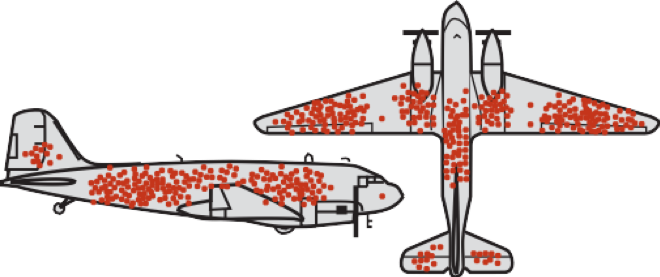
\includegraphics{AirplaneMissileHits.png}
\caption{Figure: Airplane bullet holes}
\end{figure}

\hypertarget{exercise-5}{%
\paragraph{Exercise 5}\label{exercise-5}}

An important quantity in conservation biology is the number of plant and
animal species inhabiting a given area. To survey the community of small
mammals inhabiting Kruger National Park in South Africa, a large series
of live traps were placed randomly throughout the park for one week in
the main dry season of 2004. Traps were set each evening and checked the
following morning. Individuals caught were identified, tagged (so that
new captures could be distinguished from recaptures), and released. At
the end of the survey, the total number of small mammal species in the
park was estimated by the total number of species captured in the
survey.

\begin{enumerate}
\def\labelenumi{\alph{enumi})}
\item
  What is the parameter being estimated in the survey?
\item
  Is the sample of individuals captured in the traps likely to be a
  random sample? Why or why not? In your answer, address the two
  criteria that define a sample as random.
\item
  Is the number of species in the sample likely to be an unbiased
  estimate of the total number of small mammal species in the park?
\end{enumerate}

\hypertarget{week-2-04.03.2020}{%
\subsection{Week 2 (04.03.2020)}\label{week-2-04.03.2020}}

\hypertarget{exercise-6}{%
\paragraph{Exercise 6}\label{exercise-6}}

We use the MPG data set introduced in the lecture. Answer the following
questions. You can use base R or ggplot if not otherwise specified.

\begin{enumerate}
\def\labelenumi{\alph{enumi})}
\item
  Run ggplot(data = mpg). What do you see?
\item
  How many rows are in mpg? How many columns?
\item
  What does the drv variable describe? Read the help for ?mpg to find
  out.
\item
  Make a scatterplot of hwy vs cyl.
\item
  What happens if you make a scatterplot of class vs drv? Why is the
  plot not useful?
\item
  What???s gone wrong with this code? Why are the points not blue?
\end{enumerate}

ggplot(data = mpg) +

geom\_point(mapping = aes(x = displ, y = hwy, color = ``blue''))

\begin{enumerate}
\def\labelenumi{\alph{enumi})}
\setcounter{enumi}{6}
\tightlist
\item
  Map a continuous variable to color, size, and shape. How do these
  aesthetics behave differently for categorical vs.~continuous
  variables?
\item
  Fix the following code:
\end{enumerate}

ggplot(data = mpg)

\begin{itemize}
\tightlist
\item
  geom\_point(mapping = aes(x = displ, y = hwy))
\end{itemize}

\hypertarget{week-3-11.03.2020}{%
\subsection{Week 3 (11.03.2020)}\label{week-3-11.03.2020}}

\hypertarget{exercise-7}{%
\paragraph{Exercise 7}\label{exercise-7}}

Load the data set XXX (found on ilias) and answer the following
questions and provide the R code you used for that. Put all of your
analysis in a single R script.

\begin{enumerate}
\def\labelenumi{\alph{enumi})}
\tightlist
\item
  How many individuals are in the sample (i.e., what is the sample size,
  n)?
\item
  What is the sum of all of the observations?
\item
  What is the mean of this sample?\\
\item
  What is the sum of the squares of the measurements?
\item
  What is the variance of this sample?
\item
  What is the standard deviation of this sample?
\item
  What is the coefficient of variation for this sample?
\item
  Display the data using different plotting techniques. Which one
  illustrates the data best?
\end{enumerate}

\hypertarget{week-4-18.03.2020}{%
\subsection{Week 4 (18.03.2020)}\label{week-4-18.03.2020}}

\hypertarget{exercise-8}{%
\paragraph{Exercise 8}\label{exercise-8}}

Use the stickleback dataset and calcualte the median and mean for each
genotpye. Make a histogramm and add vertical lines to the histogramm
indicating the mean and median for each genotype. What do you see? How
does the shape of the distribution affect differences between mean and
median?

\hypertarget{exercise-9}{%
\paragraph{Exercise 9}\label{exercise-9}}

Write a short R script that simulates the sampling distribution of the
mean. Plot the sampling distribution and add the theoretical expectation
to the plot. Follow the following steps:

\begin{enumerate}
\def\labelenumi{\alph{enumi})}
\tightlist
\item
  Choose a distribution that represents your population (e.g., Normal or
  Poisson).
\item
  Draw a sample of n individuals from that population (hint: use rnorm,
  rpoiss, etc.. to draw a random sample), and store it in a vector.
\item
  Calculate the mean of the sample. Store the mean of this sample in a
  vector.
\item
  Do this 1000 times, so that you have calculated a 1000 means from a
  1000 samples. Hint: use a for-loop to automate this.
\item
  Plot a histogram of the sample means.
\item
  Add a line for the theoretical expectation of the sampling
  distribution. Hint: use the function dnorm to get the density of the
  normal distribution.
\end{enumerate}

\hypertarget{week-5-25.03.2020}{%
\subsection{Week 5 (25.03.2020)}\label{week-5-25.03.2020}}

\hypertarget{exercise-10}{%
\paragraph{Exercise 10}\label{exercise-10}}

The pizza below, ordered from the Venn Pizzeria on Bayes Street, is
divided into eight slices.

\begin{figure}
\centering
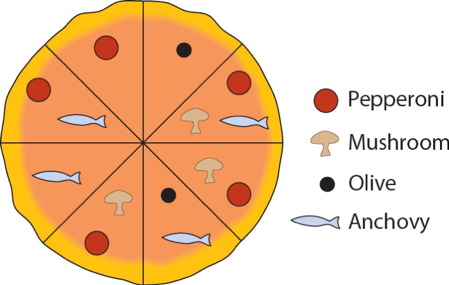
\includegraphics{Pizza.png}
\caption{Figure: Venn Pizza}
\end{figure}

Answer the following questions based on the drawing of the pizza: a)
What is the probability that a randomly drawn slice has pepperoni on it?
b) What is the probability that a randomly drawn slice has both
pepperoni and anchovies on it? c) What is the probability that a
randomly drawn slice has either pepperoni or anchovies on it? d) Are
pepperoni and anchovies mutually exclusive on this pizza? e) Are olives
and mushrooms mutually exclusive on this pizza? f) Are getting mushrooms
and getting anchovies independent when randomly picking a slice of
pizza? g) If I pick a slice from this pizza and tell you that it has
olives on it, what is the chance that it also has anchovies? h) If I
pick a slice from this pizza and tell you that it has anchovies on it,
what is the chance that it also has olives? i) Seven of your friends
each choose a slice at random and eat them without telling you what
toppings they had. What is the chance that the last slice has olives on
it? j) You choose two slices at random. What is the chance that they
have both olives on them? (Be careful ??? after removing the first
slice, the probability of choosing one of the remaining slices changes.)
k) What???s the probability that a randomly chosen slice does not have
pepperoni on it? Draw a pizza for which mushrooms, olives, anchovies and
pepperoni are all mutually exclusive

\hypertarget{exercise-11}{%
\paragraph{Exercise 11}\label{exercise-11}}

After graduating from your university with a biology degree, you are
interviewed for a lucrative job as a snake handler in a circus sideshow.
As part of your audition, you must pick up two rattlesnakes from a pit.
The pit contains eight snakes, three of which have been defanged and are
assumed to be harmless, but the other five are definitely still
dangerous. Unfortunately budget cuts have eliminated the herpetology
course from the curriculum and so you have no way of telling in advance
which snakes are dangerous and which are not. You pick one snake with
your left hand and one with your right.

\begin{enumerate}
\def\labelenumi{\alph{enumi})}
\tightlist
\item
  What is the probability that you picked up no dangerous snakes?
\item
  Assume that any dangerous snake that you pick up has a probability of
  0.8 of biting you. The defanged snakes do not bite. What is the chance
  that, in picking up your two snakes, you are bitten at least once?
\item
  If you picked up one snake and it didn???t bite you, what is the
  probability that it is defanged.
\end{enumerate}

\hypertarget{exercise-12}{%
\paragraph{Exercise 12}\label{exercise-12}}

Five different researchers independently take a random sample from the
same population and calculate a 95\% confidence interval for the same
parameter. a) What is the probability that all five researchers have
calculated an interval that includes the true value of the parameter? b)
What is the probability that at least one does not include the true
parameter value.

\hypertarget{exercise-13}{%
\paragraph{Exercise 13}\label{exercise-13}}

Use the stickleback data set. Calculate a confidence interval for the
mean plate numbers for each genotype. Make a plot that shows the mean
and the confidence interval of each genotype.

\hypertarget{week-6-01.04.2020}{%
\subsection{Week 6 (01.04.2020)}\label{week-6-01.04.2020}}

\hypertarget{week-7-08.04.2020}{%
\subsection{Week 7 (08.04.2020)}\label{week-7-08.04.2020}}

\hypertarget{week-8-21.04.2020}{%
\subsection{Week 8 (21.04.2020)}\label{week-8-21.04.2020}}

\hypertarget{week-9-28.04.2020}{%
\subsection{Week 9 (28.04.2020)}\label{week-9-28.04.2020}}

\hypertarget{week-10-06.05.2020}{%
\subsection{Week 10 (06.05.2020)}\label{week-10-06.05.2020}}

\hypertarget{week-11-13.05.2020}{%
\subsection{Week 11 (13.05.2020)}\label{week-11-13.05.2020}}

\hypertarget{week-12-20.05.2020}{%
\subsection{Week 12 (20.05.2020)}\label{week-12-20.05.2020}}

\hypertarget{week-13-27.05.2020}{%
\subsection{Week 13 (27.05.2020)}\label{week-13-27.05.2020}}


\end{document}
